% --------------------------------------------------------------
% Preamble
% --------------------------------------------------------------

\documentclass[english,natbib,man,floatsintext]{apa6}
% \usepackage{arxiv}
\usepackage[english]{babel}
\usepackage[utf8]{inputenc} % allow utf-8 input
\usepackage[T1]{fontenc}    % use 8-bit T1 fonts
\usepackage{url}            % simple URL typesetting
\usepackage{hyperref}       % hyperlinks
\usepackage{xcolor}
\hypersetup{
    colorlinks,
    linkcolor={red!50!black},
    citecolor={blue!50!black},
    urlcolor={blue!80!black}
}
\usepackage{booktabs}       % professional-quality tables
\usepackage{tabularx}
\usepackage{amsfonts}       % blackboard math symbols
\usepackage{nicefrac}       % compact symbols for 1/2, etc.
\usepackage{microtype}      % microtypography
\usepackage{gensymb}        % degree, angle symbols
\usepackage{lscape} 

% for math equations and symbols
\usepackage{amsmath} 
\usepackage{amssymb}
\newcommand{\E}{\mathbb{E}}
\newcommand{\SD}{\mathit{SD}}
\newcommand{\SE}{\mathit{SE}}
\newcommand{\BF}{\mathit{BF}}
\DeclareMathOperator\arctanh{arctanh}

% This prevents placing floats before a section.
\usepackage{placeins}

% bibliography
%\usepackage{natbib}

% allows for floats when doing jou or doc style
\usepackage{graphicx}      
\graphicspath{{./Figures/}}  
\usepackage{threeparttable}
%\usepackage{float}

% for long tables
\usepackage{longtable}
% for multitables
\usepackage{multirow}
% to rotate figures
\usepackage{rotating}
% linenumbers
\usepackage[mathlines]{lineno}
\usepackage{pdflscape}

% in APA man mode captions are too large
% making sure they are reasonable
\usepackage{setspace}
% \usepackage[font=singlespacing]{caption}
% \captionsetup{font=singlespacing}

%%% some support for commenting
\usepackage{color}
\definecolor{Blue}{RGB}{0,0,255}
\definecolor{Red}{RGB}{255,0,0}
\definecolor{Green}{RGB}{0,255,0}
\newcommand{\jdc}[1]{\textcolor{Red}{[Jacob DC: #1]}}  
\newcommand{\jlo}[1]{\textcolor{Blue}{[Jacob O: #1]}} 
\newcommand{\spe}[1]{\textcolor{Green}{[Sonja: #1]}}

% ---------------------------------------------------------
% Title, authors
% ---------------------------------------------------------

\title{How (even imperfect preregistered) research can produce false positive findings}
\shorttitle{preregistered research and false positive findings}

\fourauthors{Jacob D. Christensen*}{Jacob L. Orquin}{Sonja Perkovic}{Carl-Johan Lagerkvist}
\fouraffiliations{Swedish University of Agricultural Sciences}{Aarhus University and Reykjavik University}{Aarhus University}{Swedish University of Agricultural Sciences}

\authornote{Jacob D. Christensen, *Correspondence concerning this article should be addressed to Jacob D. Christensen, Department of Economics at Swedish University of Agricultural Sciences. E-mail: jacob.dalgaard.christensen@slu.se.}

% ---------------------------------------------------------
% Abstract
% ---------------------------------------------------------

\abstract{Even with a small number of variables researchers can test many possible models of their data thus increasing the risk of false-positive results. Using combinatorics, we show that one key independent variable and three covariates can generate 95 possible models, while six covariates can generate over 2.3 million models. Such large model sets nearly guarantee false-positive findings. Using simulation, we show that preregistering a single analysis with a key independent variable heavily reduces the risk of false-positives. However, even so many models produce false-positive results with a much higher probability than the expected 5\%. The worst-case scenario are models with interactions between binary dummy coded variables and omitted main effects. Such models can generate false-positive results up to 41.9\% of the time. While preregistration is a crucial step towards reducing false-positive results, researchers need to carefully consider what analyses they preregister and we provide recommendations for what analyses to avoid. Our findings also suggest that interpreting p-values in exploratory analyses might be meaningless considering the high false-positive probability.
}

\keywords{type I error, false-positive statistics, replicability, simulation} 

\begin{document}
\maketitle

% introduction
Imagine that you are interested in the effect of a key independent variable on a dependent variable. You are not sure whether your key variable may interact with other variables, so you decide to collect several covariate variables you think could influence your presumed causal chain. After collecting the data, you run multiple models with and without the additional variables as covariates in order to probe the data; you remove some outliers to improve the clarity of the results; and you finally find that your key variable significantly interacts with one of your covariates.
Even though, that it might seem intuitive that this kind of practice may increase false-positive findings, there seem to be a problem in some research communities with understanding the consequences of such flexibilities \citep{Makel2021,John2012,Agnoli2017,fraser2018}. 
Simulations have shown that running even a small number of models with just one covariate and its interaction, dropping conditions and having multiple dependent variables can increase the chance of a false-positive result to 60.7\% \citep{Simmons2011}, however, these questionable research practices are presumably pervasive.
Researcher flexibilities have been studied for many years and under different names, such as researcher degrees of freedom \citep{Simmons2011}, p-hacking \citep{simonsohn2014p}, data snooping \citep{white2000reality}, data mining \citep{lovell1983}, and data fishing \citep{selvin1966data}, but have received increasing attention with the open science movement \citep{banks2019answers}.   \\

Open science practices forces researchers to plan and conduct their research differently; before collecting any data, they should preregister all variables, hypotheses, sample size justification, outlier criteria, and analyses they aim to run \citep{Pham2020, Simmons2020, VANTVEER20162}. As everything is preregistered, a researcher may only run one model to test each hypothesis. Additional models or tests can still be performed and published, but are then labeled as exploratory \citep{Nosek2018}. Following this procedure, one should in principle expect to increase the replicability of research results by lowering the risk of false-positives to a preset alpha level such as the conventional level of statistical significance of 5\% \citep{Moore2016}. But can researchers rely on this procedure to entirely eliminate the increased rate of false-positive results? Probably not. \\

The 5\% chance of a false-positive result is an assumption that relies on running only one single hypothesis test and that all statistical analysis are done correctly. Previous studies have shown that misspecifying a statistical model i.e., the true model is not contained in the model set or wrong distributional assumptions are made, can increase false-positives to above the alpha level even when running a single model \citep{Dennis2019,Litiere07}. Misspecification is not the only challenge; noise in measured independent variables e.g., individuals overstating their height or socioeconomic status, can also increase the risk of false-positives \citep{Brunner2009} and so can variables with ceiling effects i.e, a large proportion of participant scores toward the high end of the scale \citep{Austin2003}. Furthermore, it has also been shown that the rate of false-positive results increases when having an interaction effect with a naturally continuous covariate which has been dichotomized \citep{Austin2004, maxwell1993bivariate}. The problem with such dichotomization is further aggravated when the sample size increases, which runs counter to the recommendation to use larger samples to minimize the risk of Type I errors \citep{simmons2018}. 
\\
It may appear tempting to dismiss these findings as irrelevant as long as we rely on sound scientific and statistical practices. However, it is easy to determine if a model is misspecified in a simulation study since we know the ground truth about the data generating process, but in reality we hardly ever know this. Can we judge the risk of model misspecification simply from the model? This might be possible in some cases such as when estimating the interaction effect, but omitting the corresponding main effect. Omitting the main effect leads to a bias in the coefficients \citep{Branbor2006} which could consequently lead to a higher rate of false-positives. The practice of estimating interactions without the corresponding main effects is widespread \citep{Branbor2006} and some method books still suggest doing this in some cases \citep{Cleves2008}. The argument is that omitting main effects is sometimes justified based on theory \citep{aiken1991multiple}. The same could be true for many other common research practices. For instance, testing models using different criteria for outlier deletion or testing several dependent variables should in principle increase false-positives due to multiple testing. However, it has also been shown that running even a single model with outlier deletion can increase the rate of false-positives if the exclusion leads to range restriction in the dependent or independent variable \citep{Raju2003}.  \\        

To conclude, the risk of false-positive results can be inflated due to two main reasons, either from testing multiple models using researcher flexibilities or due to testing a single model under conditions such as misspecification. The open science movement has largely focused on researcher flexibilities and the risk of testing multiple models whereas traditional statistical research has focused on conditions that can inflate Type I error rates when testing a single model. Judging from previous literature, both perspectives are relevant to understanding and reducing false-positive findings and integrating them may help advance our understanding of this important topic. A direct comparison may, for instance, reveal if false-positive results are more likely to arise from researchers testing multiple models or from researchers testing a single model under certain conditions. Type I error rates can be inflated by more or less common conditions such omitting main effects in interaction models, dichotomizing variables, or using outlier deletion, but how large is the risk compared to that of researcher flexibilities? In this paper, we jointly examine the risk of false-positives posed by testing multiple models and by testing a single model depending on the model specification. We define two outcome measures; the \textit{false-positive probability} and the \textit{false-positive ratio}. \\
Previous research on researcher flexibilities has examined the false-positive probability \citep{Simmons2011}, which is the chance of erroneously finding one or more significant effects among all the tested ones. The false-positive probability reveals problems with conducting multiple tests and with flexible research practices in general, but it does not provide information on how many of the tested models contain a significant effect. For example, with one key variable and three covariates it is possible to test 95 models\footnote{Equations for calculating this number is shown later in the paper}. If just one of these models produces a false-positive then the false-positive probability is 100\%. However, the risk of running that one offending model is rather small and would require a concerted effort to test a large number of the possible models. On the other hand, if 25 of the 95 possible models produce false-positives the risk is much higher. To understand this latter aspect, we examine the false-positive ratio, which we define as the number of models with a significant key variable effect within a given set of models. Both measurements provide information about the the risk of false-positives, but under different conditions: the false-positive probability inform us about the likelihood that a researcher can generate a false-positive result when testing a large number of models, whereas the false-positive ratio informs us about the risk of producing a false-positive result when testing a single model such as when following a preregistered research plan. \\

In this article, we report the results of a simulation study on the false-positive probability and false-positive ratio for different types of regression models. 
To this end, we first develop a combinatorial analysis of all possible regression models that a researcher can test with a single variable of interest and a given number of covariates. We show how the total set of all possible models can be decomposed into seven subsets e.g., the set of models with main effects only, the set of models with interaction effects between variable of interest and covariates, the set of models with interactions between covariates, and the sets that combine sets.  
In our simulation, we examine the models sets separately and under different conditions such as changes in the correlation between the covariates and the dependent variable, different types of data structure (binary and continuous variables), and larger sample sizes.
Our results show that producing a false-positive effect is not difficult, but merely a matter of testing enough models as the false-positive probability can reach just below 100\% in some model sets. More importantly, our results show that testing a single preregistered model does not bind the false-positive ratio to 5\% as many model sets have an inflated false-positive ratio. Finally, a larger sample does not help reduce the risk of false-positive results, and in some cases even makes it worse.
Our analysis brings together two streams of literature: one concerned with researcher flexibilities and the other one concerned with type I error rates due to specific conditions such as model misspecification. Our results show that both perspectives are necessary to advance science in terms of replicability since current open-science practices may not be a sufficient safeguard against false-positive results; some types of analyses can inflate the risk of false-positive results even when preregistered. 
 \\ 
 


% method section
\section{Method}
Focusing on different flexibilities in data analysis, we investigated the false-positive probability (FPP) and false-positive ratio (FPR) for a key independent variable that was uncorrelated with any other variable using a simulation. We used the previously discussed flexibilities i.e., different model specifications, outlier deletion present or absent, several dependent variables, and different sample sizes. The effect of flexibilities were tested using different correlations between the dependent variable and the covariates, and different data structures. Even though in some simple cases it would be possible to calculate a closed-form solution for the FPP and FPR e.g., when looking at only one main effect, we used a simulation since it was not clear how the combination of different flexibilities would impact the FPP and FPR.\\

\subsection{Model Set}
When a researcher has to select which model(s) to use for testing a hypothesis, there are a lot of possibilities regarding what variables to collect and how they should enter the model. In a completely randomized experiment, it would only be necessary to focus on the key variable of interest, which we define as $x_1$, and the dependent variable, $y$ \citep{angrist2008mostly}. However, in many cases a researcher is either interested in how the variable of interest interacts with other variables or there is a need to control for other variables, which we call covariates and denote as $Z=(z_1,z_2,..,z_n)$. For instance, this could be the case in a quasi-experimental setting where no complete randomization could be obtained or for observational data where it is necessary to control for different variables to avoid bias \citep{angrist2008mostly}. \\ 
To better understand the construction of model sets, we divided the models into seven sets based on different interaction structures. The first three sets contained the key variable of interest and simple interactions, whereas the last four sets were the combinations of the first three sets. For clarity, the model equations exclude the constant and the coefficient in front of each variable. The first set only includes models of the main effects of the variable of interest and the covariates ($x + z$). The second set includes models with a main effect of the variable of interest and interactions between the variable of interest and the covariates ($x \times z$). The third set includes models with a main effect of the variable of interest and covariate-covariate interactions ($z \times z$).
To obtain the last four model sets, we combine the first three model sets. There are two ways of developing the model sets: with restrictions on main effects and without restrictions on main effects. Restrictions on main effects mean that whenever there is an interaction term the corresponding main effect terms have to be included in the model. Models without restrictions on the other hand are allowed to include interaction terms without the corresponding main effect terms. In Table \ref{modelsets2.1}, we show examples of all model sets with one variable of interest, $x_{1}$, and two covariates, $z_{1}$ and $z_{2}$, depending on the main effect restriction. \\
 
\begin{table}[!htbp]
\centering
\caption{}
\caption*{\footnotesize An overview of all of the model sets when there are two covariates and one dependent variable with the restriction that main effects should be present when having interactions between variables (column two) and with no restrictions that main effects must follow interactions (column three). The ME set contains all of the main effects; the $ME + X \times Cov$  set includes the main effects and interactions between the variable of interest and the covariates; the $ME + Cov \times Cov$ set contains the main effects and  interactions between the covariates; the $ME + X \times Cov + Cov \times Cov$ set contains the main effects, the interactions between the variable of interest and covariates, and the interactions between the covariates; the $X \times Cov$, $Cov \times Cov$ and $X \times Cov + Cov \times Cov$ sets are empty sets when there is restrictions on our interactions since they only contain the interactions but not the required main effects.}
\label{modelsets2.1}
\begin{threeparttable}
\scalebox{0.85}{%
\begin{tabular}{ccc}
\hline
Model set & Models with restrictions & Models without restrictions \\ \hline
ME & \begin{tabular}[c]{@{}c@{}}$y=x_1$\\  $y=x_1+z_1$\\  $y=x_1+z_2$ \\  $y=x_1+z_1+z_2$\end{tabular} & \begin{tabular}[c]{@{}c@{}}$y=x_1$\\  $y=x_1+z_1$\\  $y=x_1+z_2$ \\  $y=x_1+z_1+z_2$\end{tabular} \\
$X \times Cov$ & Empty set & \begin{tabular}[c]{@{}c@{}}\rule{0pt}{5ex}$y=x_1+x_1z_1$ \\ $y=x_1+x_1z_2$\\ $y=x_1+x_1z_1+x_1z_2$\end{tabular} \\
$Cov \times Cov$ & Empty set & \rule{0pt}{5ex}$y=x_1+z_1z_2$ \\
$ME + X \times Cov$ & \begin{tabular}[c]{@{}c@{}}$y=x_1+z_1+x_1z_1$  \\ $y=x_1+z_2+x_1z_2$ \\ $y=x_1+z_1+z_2+x_1z_1$  \\ $y=x_1+z_1+z_2+x_1z_2$  \\ $y=x_1+z_1+z_2+x_1z_1+x_1z_2$\end{tabular} & \begin{tabular}[c]{@{}c@{}}\rule{0pt}{5ex}$y=x_1+z_1+x_1z_1$\\ $y=x_1+z_1+x_1z_2$\\ $y=x_1+z_1+x_1z_1+x_1z_2$\\ $y=x_1+z_2+x_1z_1$\\ $y=x_1+z_2+x_1z_2$\\ $y=x_1+z_2+x_1z_1+x_1z_2$\\ $y=x_1+z_1+z_2+x_1z_1$\\ $y=x_1+z_1+z_2+x_1z_2$\\ $y=x_1+z_1+z_2+x_1z_1+x_1z_2$\end{tabular} \\
$ME + Cov \times Cov$ & $y=x_1+z_1+z_2+z_1z_2$ & \begin{tabular}[c]{@{}c@{}}\rule{0pt}{5ex}$y=x_1+z_1+z_1z_2$\\ $y=x_1+z_2+z_1z_2$\\ $y=x_1+z_1+z_2+z_1z_2$\end{tabular} \\
$X \times Cov + Cov \times Cov$ & Empty set & \begin{tabular}[c]{@{}c@{}}\rule{0pt}{5ex}$y=x_1+x_1z_1+z_1z_2$\\ $y=x_1+x_1z_2+z_1z_2$\\ $y=x_1+x_1z_1+x_1z_2+z_1z_2$ \end{tabular} \\  
$ME + X \times Cov + Cov \times Cov$ & \begin{tabular}[c]{@{}c@{}}$y=x_1+z_1+z_2+x_1z_1+z_1z_2$ \\ $y=x_1+z_1+z_2+x_1z_2+z_1z_2$ \\ $y=x_1+z_1+z_2+x_1z_1+x_1z_2+z_1z_2$\end{tabular} & \begin{tabular}[c]{@{}c@{}}\rule{0pt}{5ex}$y=x_1+z_1+x_1z_1+z_1z_2$\\ $y=x_1+z_1+x_1z_2+z_1z_2$\\ $y=x_1+z_1+x_1z_1+x_1z_2+z_1z_2$\\ $y=x_1+z_2+x_1z_1+z_1z_2$\\ $y=x_1+z_2+x_1z_2+z_1z_2$\\ $y=x_1+z_2+x_1z_1+x_1z_2+z_1z_2$\\ $y=x_1+z_1+z_2+x_1z_1+z_1z_2$\\  $y=x_1+z_1+z_2+x_1z_2+z_1z_2$\\ $y=x_1+z_1+z_2+x_1z_1+x_1z_2+z_1z_2$\end{tabular} \\ \hline
\end{tabular}
}%
\end{threeparttable}

\end{table}

Equation (1) shows how to calculate the total number of models given one key variable of interest and a given number of covariates with the main effects restriction that models with interaction terms must include the corresponding main effects. Each underlined section in Equation (1) can also be used to calculate the size of the specified model set. The derivation of this equation can be found in the \textit{Appendix}. \\

\begin{equation} 
\begin{aligned}
\#\ models={} & \underbrace{\left(2^n\right)}_{x + z}+\underbrace{\sum^n_{j=1}{\left(2^j-1\right)\binom{n}{j}}}_{x + z + x \times z} + \\ 
& \underbrace{\sum^n_{j=2}{\binom{n}{j}\left(2^{\frac{j\left(j-1\right)}{2}}-1\right)}}_{x + z + z \times z} + \\
& \underbrace{\sum^n_{j=2}{\binom{n}{j}\left(2^j-1\right)\left(2^{\frac{j\left(j-1\right)}{2}}-1\right)}}_{x + z + x \times z + z \times z}\ \  
\end{aligned}
\end{equation} 
where $n$ denotes the number of covariates (all the $z$ variables) collected and $\binom{n}{j}$ is the binomial coefficient, the calculation of which is explained in the \textit{Appendix}.
Equation (1) does not include the ($x \times z$), ($z \times z$), and ($x \times z + z \times z$) sets as these include interaction terms without the corresponding main effect terms, and these are therefore empty sets. For the case with two covariates, the total number of models is calculated as follows:

\begin{equation*}
\centering
\left(2^2\right)+
\sum^2_{j=1}{\left(2^j-1\right) \binom{2}{j}}+
\sum^2_{j=2}{\binom{2}{j}\left(2^{\frac{j\left(j-1\right)}{2}}-1\right)}+  
\sum^2_{j=2}{\binom{2}{j}\left(2^j-1\right)\left(2^{\frac{j\left(j-1\right)}{2}}-1\right)}
\end{equation*}

which is equal to $4+5+1+3*1=13$. The number of models in each model set for different numbers of covariates depending on main effect restrictions can be seen in Table \ref{FullModel}. In the simulation, we focus on two to three covariates since this is enough to provide an impression of how the increase in the size of the model set affects the FPP and FPR.  \\

% latex table generated in R 4.0.0 by xtable 1.8-4 package
% Tue Jan 19 16:32:31 2021
\begin{table}[!h]
\centering
\caption{The total number of models for any given set considering the different number of covariates, with and without restriction that main effects should be present when having interaction effects.} 
\label{FullModel}
\begin{tabular}{lccccc}
  \hline
  & \multicolumn{5}{c}{Number of covariates} \\\cmidrule{2-6}
With restrictions & 2 & 3 & 4 & 5 & 6 \\ 
  \hline
$x + z$ & 4 & 8 & 16 & 32 & 64 \\ 
  $x + z + x \times z$ & 5 & 19 & 65 & 211 & 665 \\ 
  $x + z + z \times z$ & 1 & 10 & 97 & 1418 & 40005 \\ 
  $x + z+ x \times z + z \times z$ & 3 & 58 & 1159 & 36958 & 2269799 \\
  \hline 
  Number of total models & 13 & 95 & 1337 & 38619 & 2310533 \\ 
  \hline \\
  Without restrictions \\ 
  \hline
  $x + z$ & 4 & 8 & 16 & 32 & 64 \\ 
  $x \times z$ & 3 & 7 & 15 & 31 & 63 \\ 
  $z \times z$ & 1 & 4 & 32 & 512 & 16384 \\ 
  $x + z + x \times z$ & 9 & 49 & 225 & 961 & 3969 \\ 
  $x + z + z \times z$ & 3 & 49 & 945 & 31713 & 2064321 \\ 
  $x \times z + z \times z$ & 3 & 49 & 945 & 31713 & 2064321 \\ 
  $x + z + x \times z + z$ \times z & 9 & 343 & 14175 & 983103 & 130052223 \\ 
  \hline
  Number of total models & 32 & 509 & 16353 & 1048065 & 134201345 \\ 
   \hline 
\multicolumn{6}{p{13cm}}{\footnotesize{Note: $x + z$ = models with main effects only; $x \times z$ = models with interactions between the variable of interest and covariates; $z \times z$ = models with interactions between covariates;  $x + z + x \times z$ = models with main effects and interactions between the variable of interest and covariates; $x + z + z \times z$ = models with main effects and interactions between covariates; $x \times z + z \times z$ = models with interactions between covariates and variable of interest and interactions between covariates; $x + z + x \times z + z \times z$ = models with main effects and interactions between the variable of interest and covariates and the interactions between covariates.}} 

\end{tabular}
\end{table}



\subsection{Outlier Criteria}
Following the findings of \cite{Leyes2013}, we included four different outlier criteria. Three of the criteria were based on the standard deviation ($SD = 2$, $SD = 2.5$, and $SD = 3$), and the remaining criterion used the interquartile range \citep{Rousseeuw2011}. Outlier criteria were applied to all variables in a dataset by omitting all observations that exceeded the outlier criteria from the analysis. 

\subsection{Multiple Dependent Variables}
As in \cite{Simmons2011}, we tested the effect of using more than one dependent variable on the FPP and FPR. We simulated data with two correlated dependent variables $r=0.5$ and computed the average of the two dependent variables to yield a third dependent variable. With these three dependent variables, the model set expanded three times compared to only one dependent variable. 

\subsection{Data Generating Process}
As the goal of the simulation was to understand what can lead to false-positive results, the variable of interest was simulated without any correlation with either the dependent variable or any of the covariates. The variable of interest could either have a normal distribution (continuous variable) or a binomial distribution (binary variable). The covariates were simulated using the same distribution so that all covariate distributions in a dataset were either normal or binomially distributed. As our target analysis was linear regression, the dependent variable was always simulated as a normal distribution. There were four different combinations of the variable of interest $x$ and covariate $z$ distributions: $x$ and $z$ are continuous, $x$ and $z$ are binary, $x$ is continuous and $z$ is binary, $x$ is binary and $z$ is continuous. The correlation between the dependent variable and covariates was simulated with three different levels (\textit{r} = 0.2, \textit{r} = 0.3, and \textit{r} = 0.4) corresponding to medium-strength correlations \citep{Cohen1989}. The correlation between the variable of interest and the covariates as well as the correlation between the covariates themselves was always set to zero. The correlation matrix for the data structure when there is only one dependent variable is presented in Table \ref{tab:correlation} in the \textit{Appendix}. If a variable was generated as a normally distributed variable, it was generated with a mean of 0 and a standard deviation of 1, while binomial variables were generated with a 50\% chance of success in each trial. To test how the sample size affected the FPP and FPR, the simulation included samples with sizes ranging from 100 to 300 with increasing steps of 50. 

\subsection{Simulation}
In the simulation results presented in the main results section, we only included cases in which the variable of interest and covariates had the same distribution. The two other cases i.e., when the variable of interest was binary and the covariates were continuous and the other way around can be found in the online \textit{Supplementary Information}. For analyses not addressing the effect of sample size, the default sample size was kept constant at 200. When the effect of different correlation levels between covariates was not analyzed, the correlation between the dependent variable and covariates was set to a default of $r=0.2$. We did not apply any outlier deletion except when outlier deletion was the focus of the simulation.\\
We used R \citep{Team2018} to perform our simulation with 10,000 simulation iterations. When the covariates had a binomial distribution, the variables were simulated using the package BinNor \citep{Demirtas2014}. The data were analyzed with linear regressions. We defined a false-positive result as any model where the variable of interest was significant ($p < .05$), either in a main effect or in an interaction with a covariate variable. The FPP was defined as \\

\[FPP_i=\left. \left\{\begin{array}{c}
1\ if\ any\ model\ in\ iteration\ i\ produces\ a\ false-positive\ result \\ 
0\ otherwise\  \end{array}
\right.\] 
\[FPP=\frac{\sum_{i}^{N}{FPP_i}}{N}\] 

The FPR is the ratio of the models with a false-positive result and was defined as \\

\[FPR_i=\frac{\#\ false-positive\ models\ in\ iteration\ i}{\#\ all\ models\ in\ the\ set\ in\ iteration\ i}\] 
\[FPR=\frac{\sum_{i}^{N}{FPR_i}}{N}\] 





% results section
\section{Results} 
To make the simulation easy to understand we started with the baseline model with two covariates that was split into the different model sets. We then started adding the different flexibilities one at a time to see how much each flexibility by itself would add to the FPP and FPR compared to the baseline model. Figure 1 shows the FPP and FPR for the baseline model with different data structures whereas the remaining figures in the result section can be seen as added effect regarding the different flexibilities. 
\subsection{Worst case scenario}
Under different conditions, the FPP was as high as 99\%. There were several ways to obtain a result like this. In general, the covariates needed to be binary and dummy coded and interactions used without including main effects. In such case, a 99\% FPP could be obtained with only two covariates and a big enough sample (see Figure 4). Alternatively, a 99\% FPP could also be obtained using a smaller sample and more than two covariates (see Figure 3). In the same sets, the FPR was as high as 35\%. In other words, in the sets where there was a 99\% chance to find a significant result, around 35\% of the models had either a significant main effect or interaction effect with the variable of interest. 

\subsection{Effect of model specification}
The FPP and FPR for the different model sets can be found in Figure 1. Looking at the FPP and FPR between the different sets, it is clear that the highest FPP and FPR could be obtained in the sets HCI and ME+ HCI. This was the case both when the main effects were present or not. When the main effects were not present, and the covariates and variable of interest were binary with dummy coding, the high FPP and FPR occurred because the interaction was only splitting the sample, and the true effect from the covariate was captured in the interaction. The FPP for a sample of 200 was 83.4\% for the HCI set and 86.9\% for the ME+ HCI set. When the variables were continuous and everything else equal, the FPP for the two sets was 18.9\% and 24.3\%, respectively. When we implemented the restriction that main effects should follow interactions, only the ME+ HCI set remained because the HCI set became an empty set. In that case, the FPP was 20.6\% for binary variables and 18.6\% for continuous variables. Across all sets the FPP for using two binary variables was 87.2\%, and for continuous, it was 24.7\% when we had no restrictions regarding the main effect and 22\% and 18.5\% respectively when we had such a restriction. 
Not only was the FPP high, but the FPR was also higher in some sets (see red bars in Figure 1). In general, the proportion of these models was around the expected 5\%, but in sets where there were interactions between the variable of interest and main effect was not present (left hand side of Figure 1), the FPR was above the 5\%. The percent of models with a significant variable of interest or interaction with the variable of interest was 31.9\% for the ME+ HCI set when main effects were not included and binary data was used. One way to remedy this was by coding the binary variables using effects coding. Here, the FPP fell to 20.6\%, and FPR in the ME+ HCI set dropped to 9.7\%, the same level as if the covariates were continuous (see Figure SI1 A in Supplementary information). Overall, the sets where HCI was included had a higher number of models with a significant effect. 
Adding one more covariate (such that the analysis included three) to the analysis just increased the FPP across all model sets, where it was still possible to get a higher FPP. This added effect of using one more covariate can be seen in Figure 2. The increase was the highest for the binary data and where there was no restriction that the main effect should follow the interaction. Several of the sets here had the rate of FPP just below a 100\%. This increase was also seen when we restrict the sets such that the main effects should always be present. Here the increase of adding one more covariate was 14.3\% to the FPP for the set ME+ HCI + CCI with binary data and 13.1\% for continuous data in the same set. The rates of FPR also increased. This increase, however, only applies for the sets where there were interactions between the variable of interest and the covariates. Even though there was a higher increase when there was no restriction that the main effect should be present, we observed a increase even when the restriction was present. Using three covariates increased the FPR for ME+ HCI + CCI for around 3\% compared to using two covariates with both binary and continuous data. 

% plot of main analysis
\begin{figure}[t]
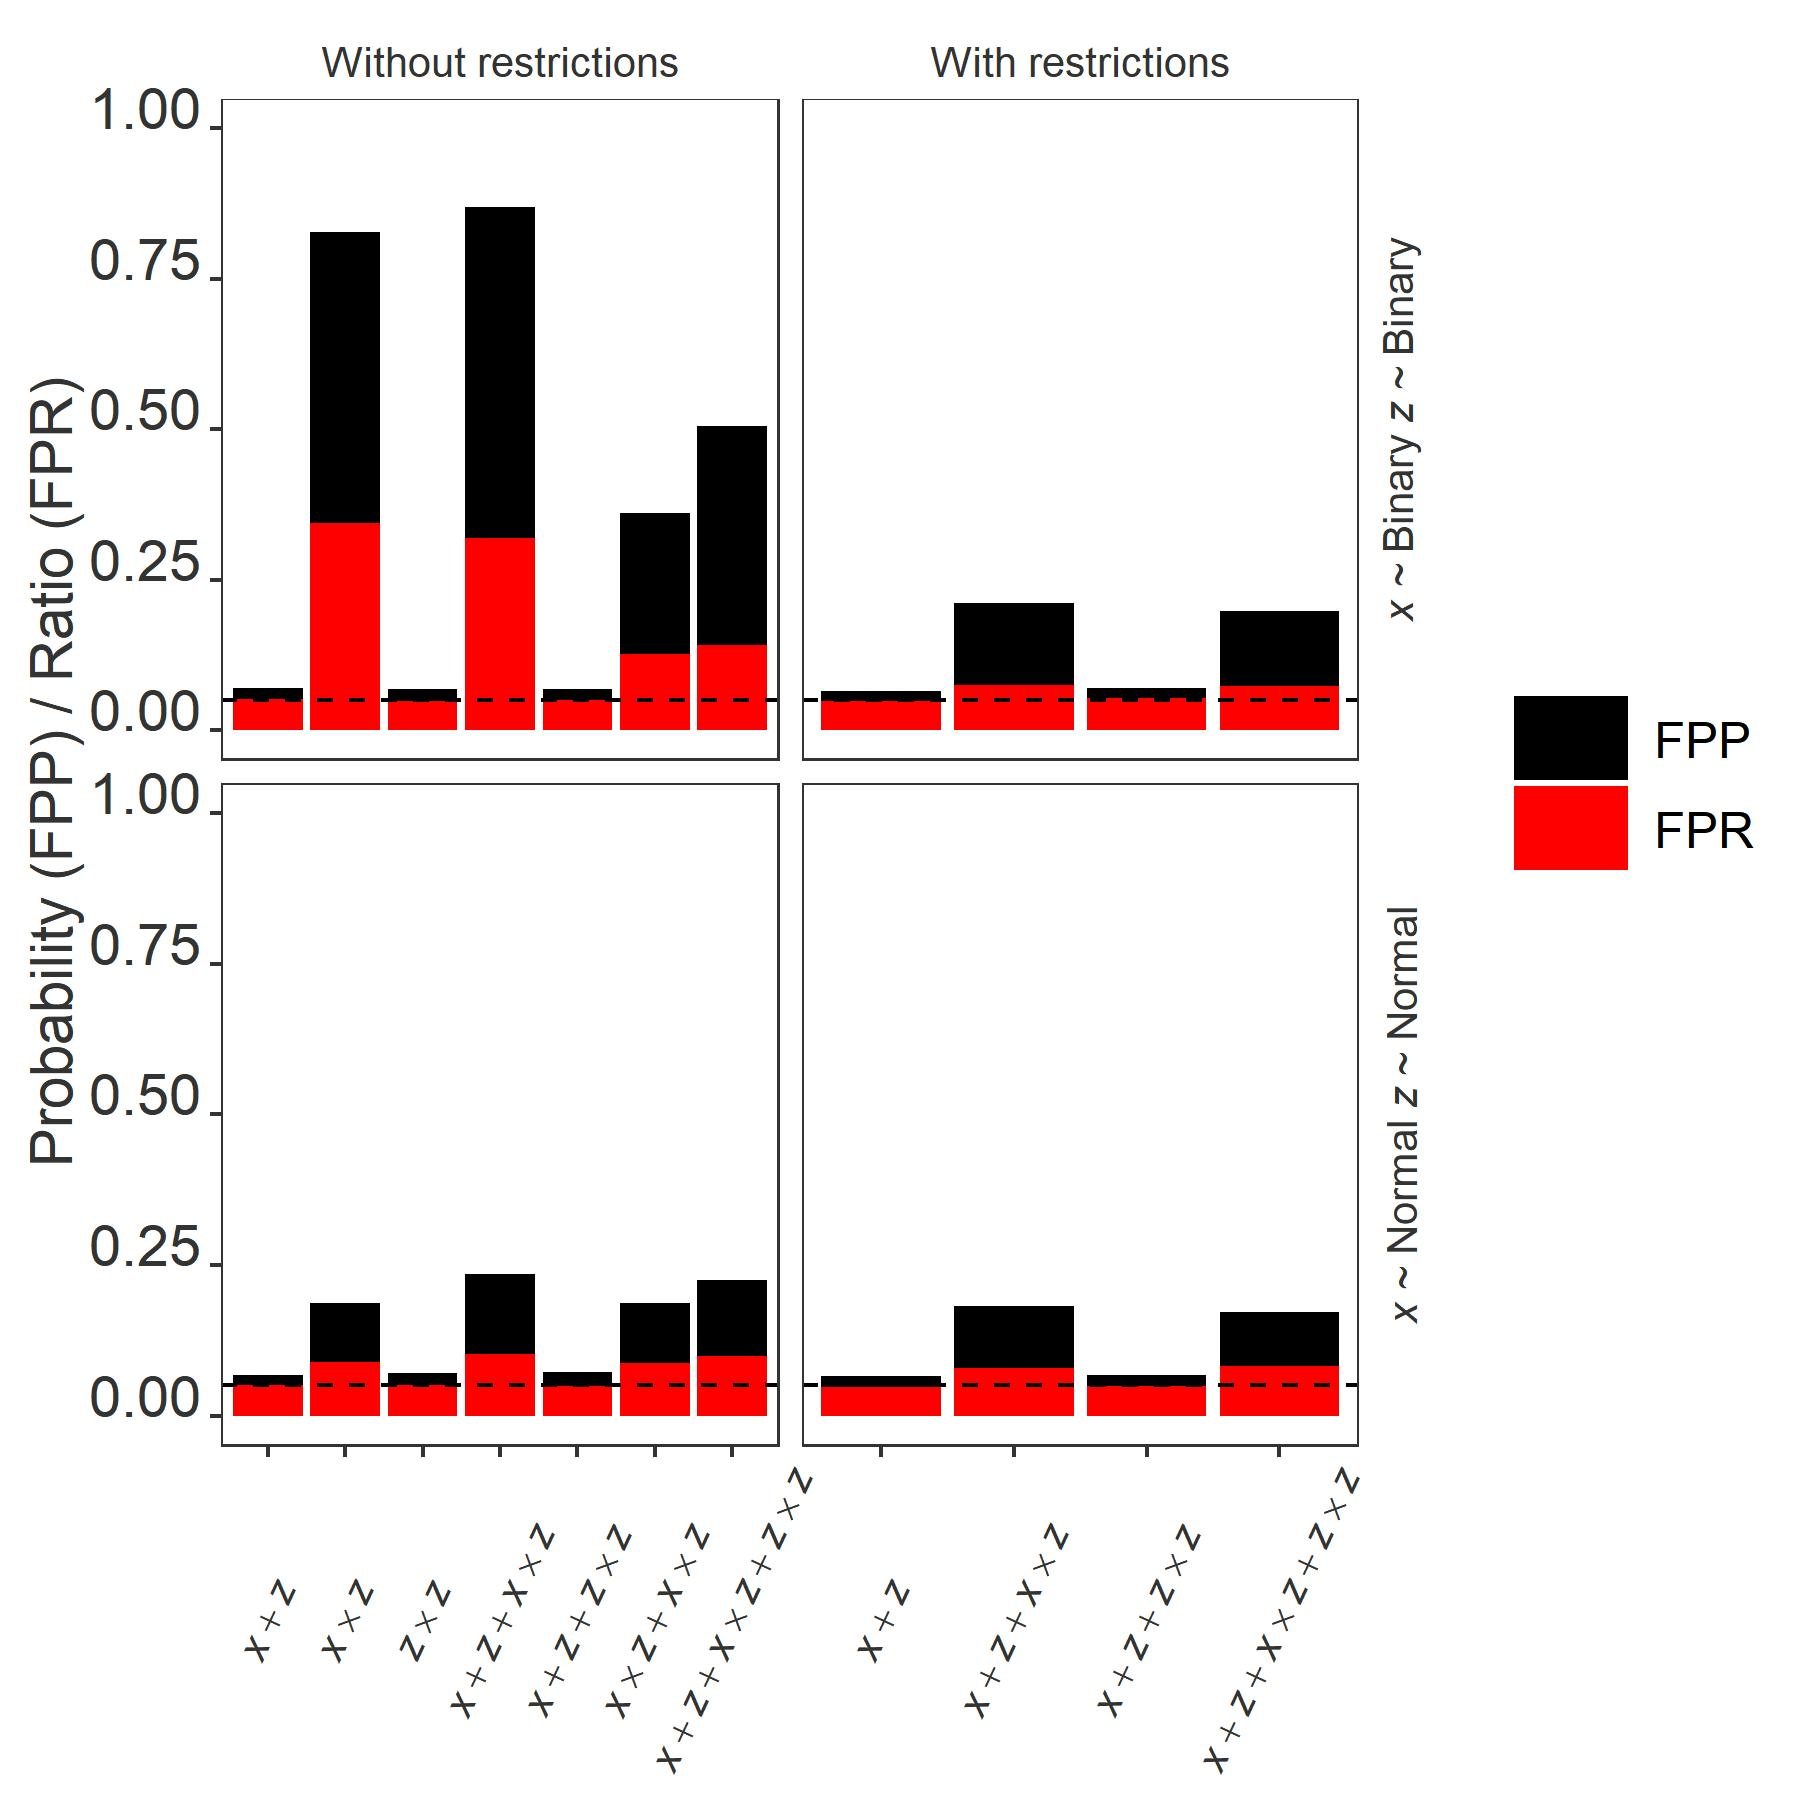
\includegraphics[width=0.6\textwidth]{R/Analysis/Result/Figures/Figure1A.jpeg}
\centering
\caption{The probability of the FPP and FPR given different model sets, the presence of main effects when having interactions and variable of interest distributions. Sample size was set to 200, a correlation between the dependent variable and covariates was \textit{r}=0.2 and we used two covariates. The FPP is shown in black and the FPR in red.}
\label{fig:mainfigure}
\end{figure}

% plot of main analysis
\begin{figure}[t]
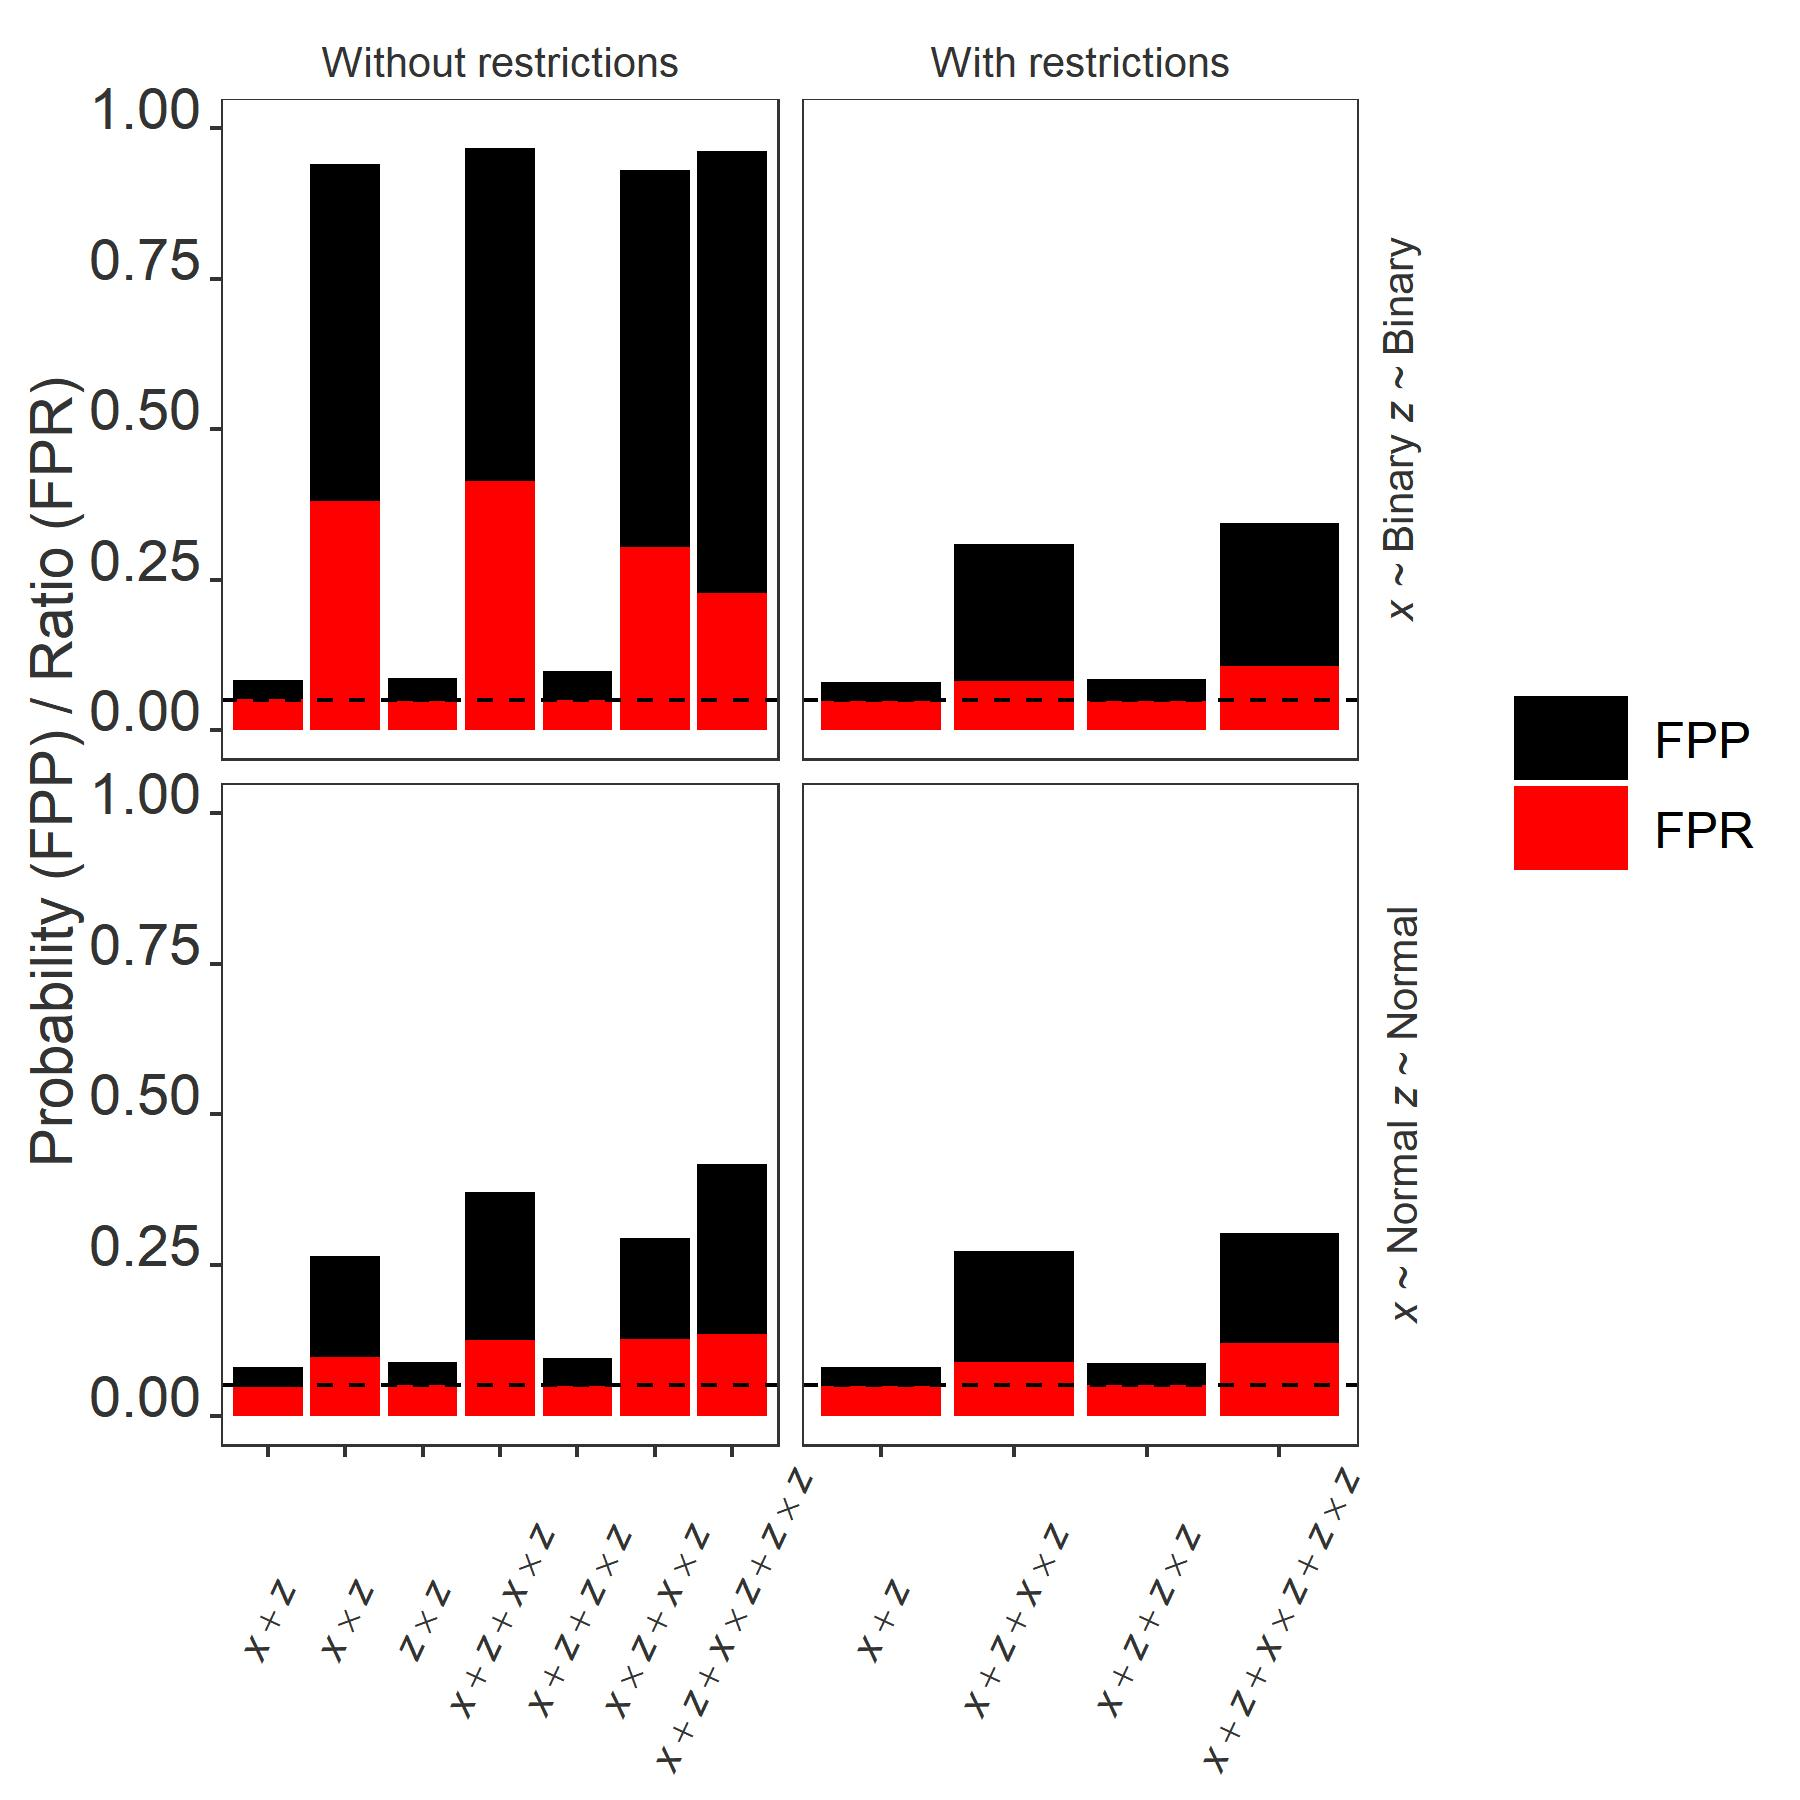
\includegraphics[width=0.6\textwidth]{R/Analysis/Result/Figures/Figure1C.jpeg}
\centering
\caption{Added effect of using one more covariate (three in total) on the FPP and FPR. The description of the figure is otherwise the same as for Figure 1.}
\label{fig:mainfigure}
\end{figure}

\subsection{Outlier criteria}
Here we were interested in how outlier deletion affected the FPP and FPR across the different model sets. Therefore, we plotted the added effect of using the four different outlier criteria compared to not using any such criteria. Again, the sample was set to 200, and all binary variables where dummy coded. Figure 3 shows the added effect of using the outlier criteria. It can be seen that outlier deletion had a different added effect on the different model sets and data structures. The main contribution was within the sets where there were interactions between the covariates. Overall, the added effect to the FPP was between 4\% and 19.4\% for model sets where there was still room for an added effect. The lower added effects seen in some cases came from the fact that the FPP was already close to 100\%. This was the case for the sets where the variables were binary and there was an interaction between the variable of interest and the covariates and where we allowed for models that did not have the main effect present. Using outlier criteria did not increase the FPR and in some cases deleting outliers even decreased the FPR. 

\begin{figure}[t]
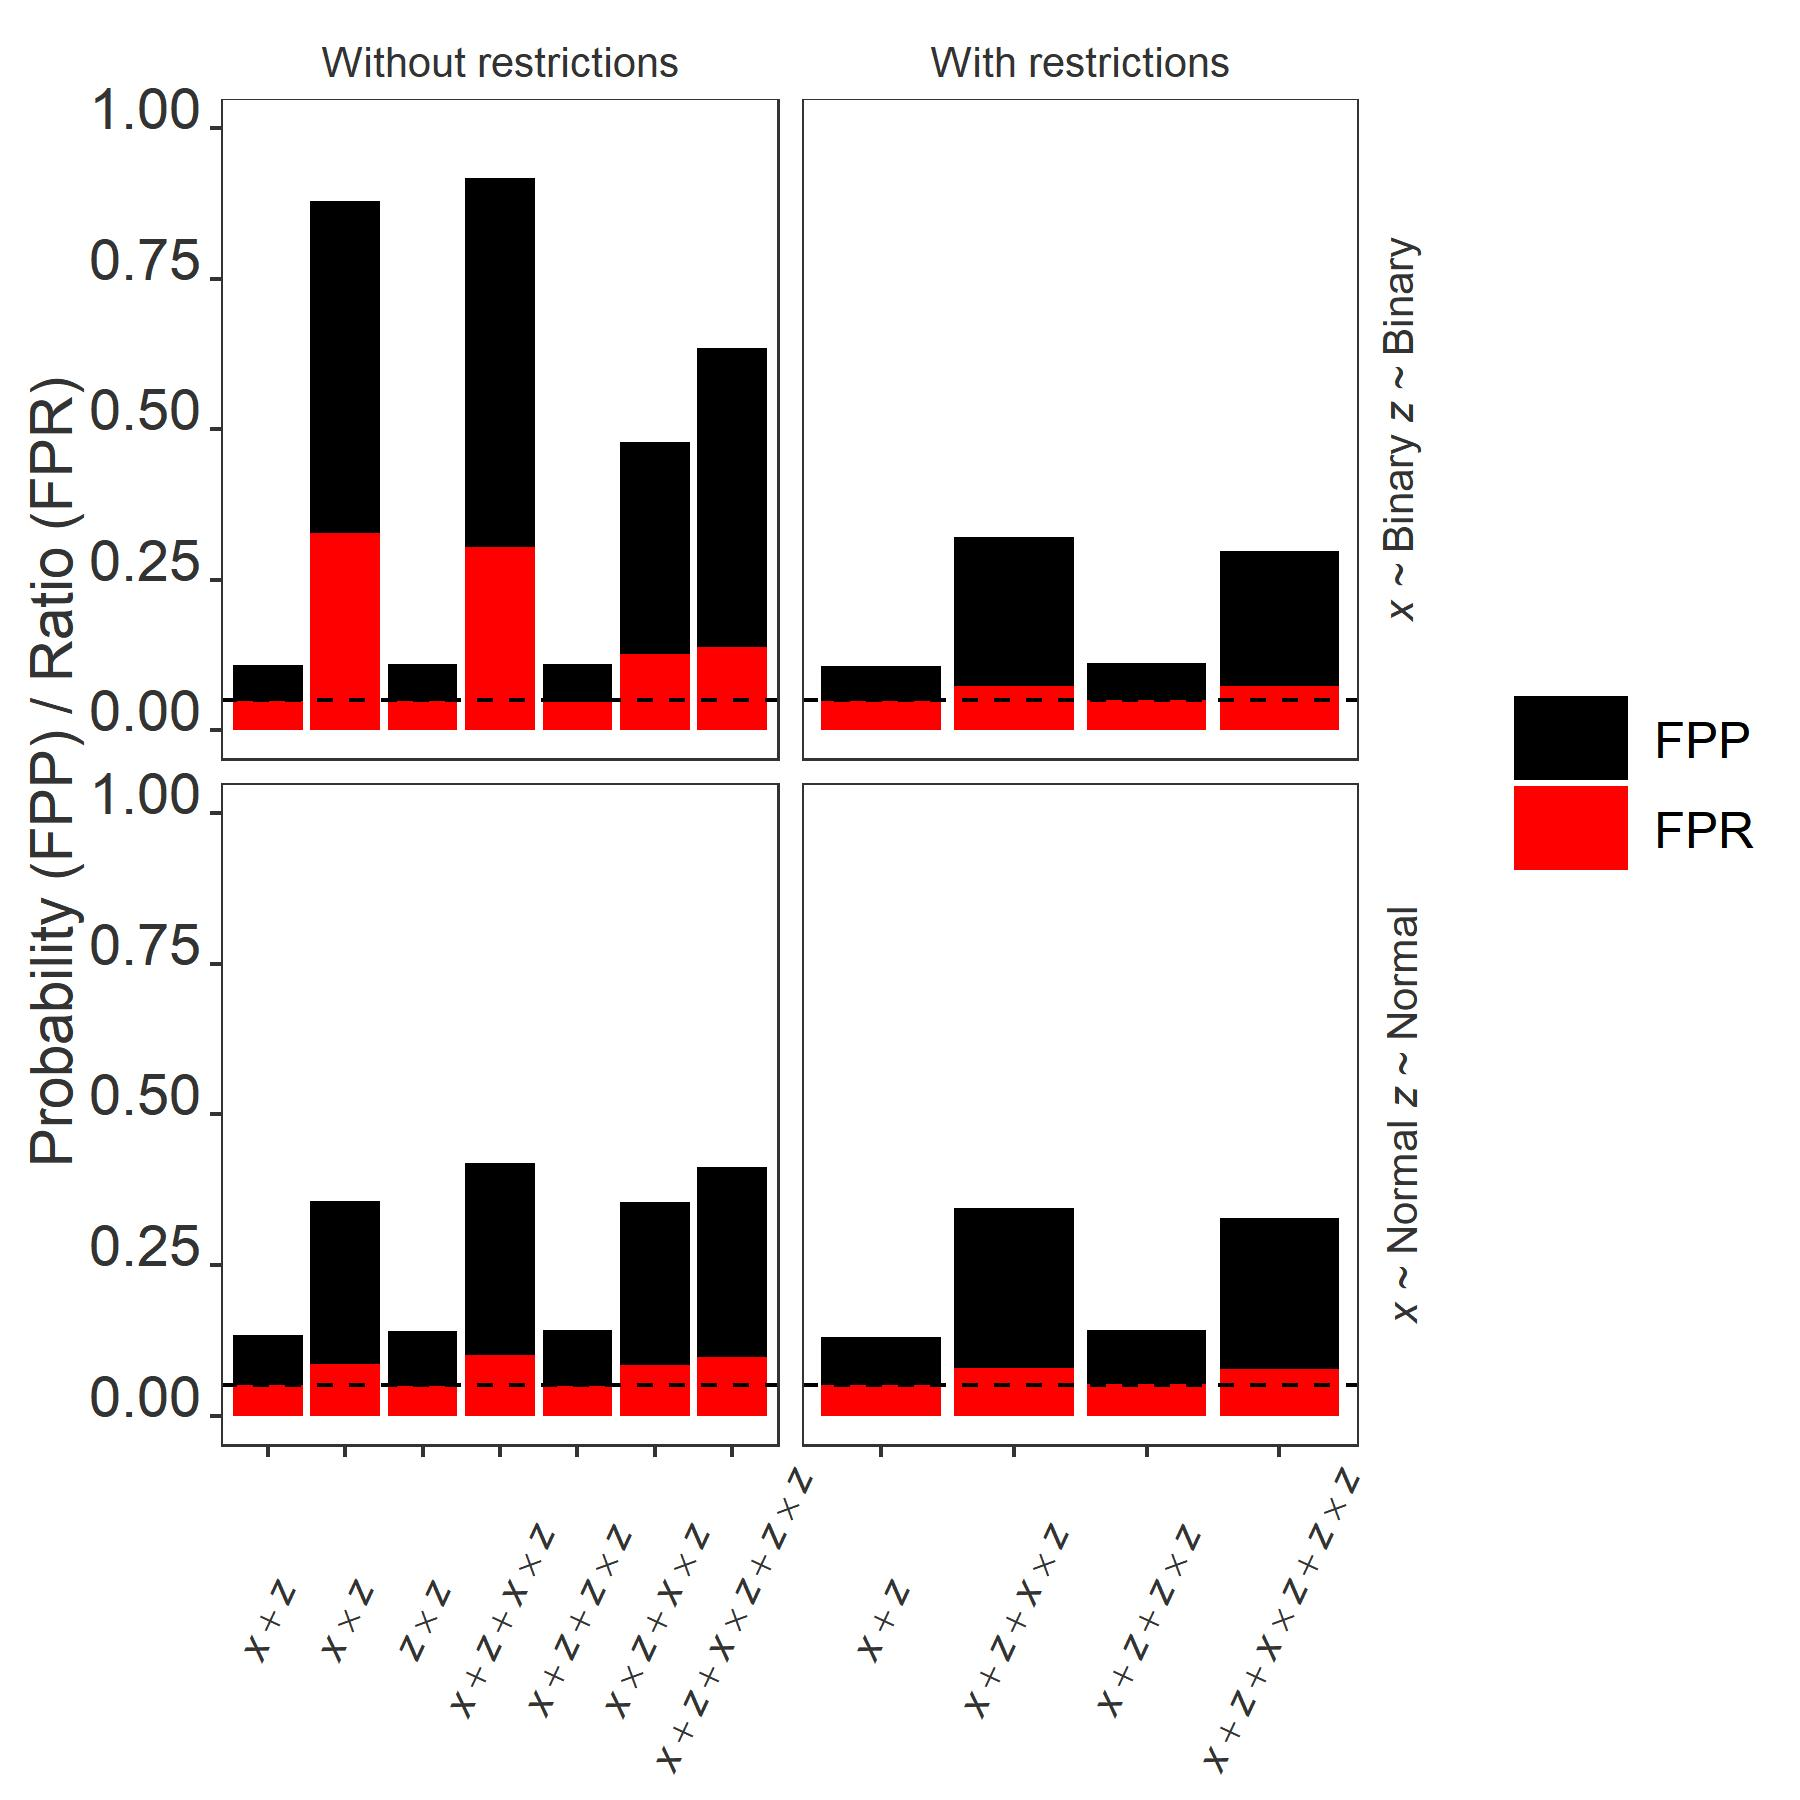
\includegraphics[width=0.6\textwidth]{R/Analysis/Result/Figures/Figure1B.jpeg}
\centering
\caption{Added effect of using multiple outlier criteria. Black denotes the added effect to the FPP and red denotes the added effect to the FPR.  The description of the figure is otherwise the same as for Figure 1.}
\label{fig:mainfigure}
\end{figure}

\subsection{Multiple dependent variables}
Here we looked at the effect of having multiple dependent variables on the FPP and FPR across different sets of the models. We did not specify any outlier criteria and all binary variables were dummy coded. Collecting multiple dependent variables and using their average increased the FPP. This was a general result regardless of data structures, model sets, and whether main effects were included or not. The effect of using two dependent variables and their average can be seen in Figure S3 in supplementary information. This increase was the highest for the sets where there were interactions between the variable of interest and the covariates, no matter the data structure and other specifications. For these sets, the increase in the FPP was around 15\%. The increase in the FPR seems to be mainly driven by the increase in the number of models, as the FPR did not increase for any of the sets. 

\subsection{Sample size}
Increasing the sample size and thereby the precision of the estimates did not seem to lower the FPP. Even worse, when the main effects were not included, the larger sample size increased the FPP when there was interactions between variable of interest and covariate and these were binary (See Figure 4). In this case, the FPP went just under 100\% as the sample size increased to 300. The larger sample did not only increase the FPP, but also the FPR. The FPR got as high as 42\% for the HCI set with binary data and no restrictions. For continues covariates, the results looked the same regardless of main effects following interactions or not, but there was still no decrease in FPP and FPR from increasing the sample size (i.e., the FPP and FPR remained roughly the same for all tested sample sizes). 


\begin{figure}[t]
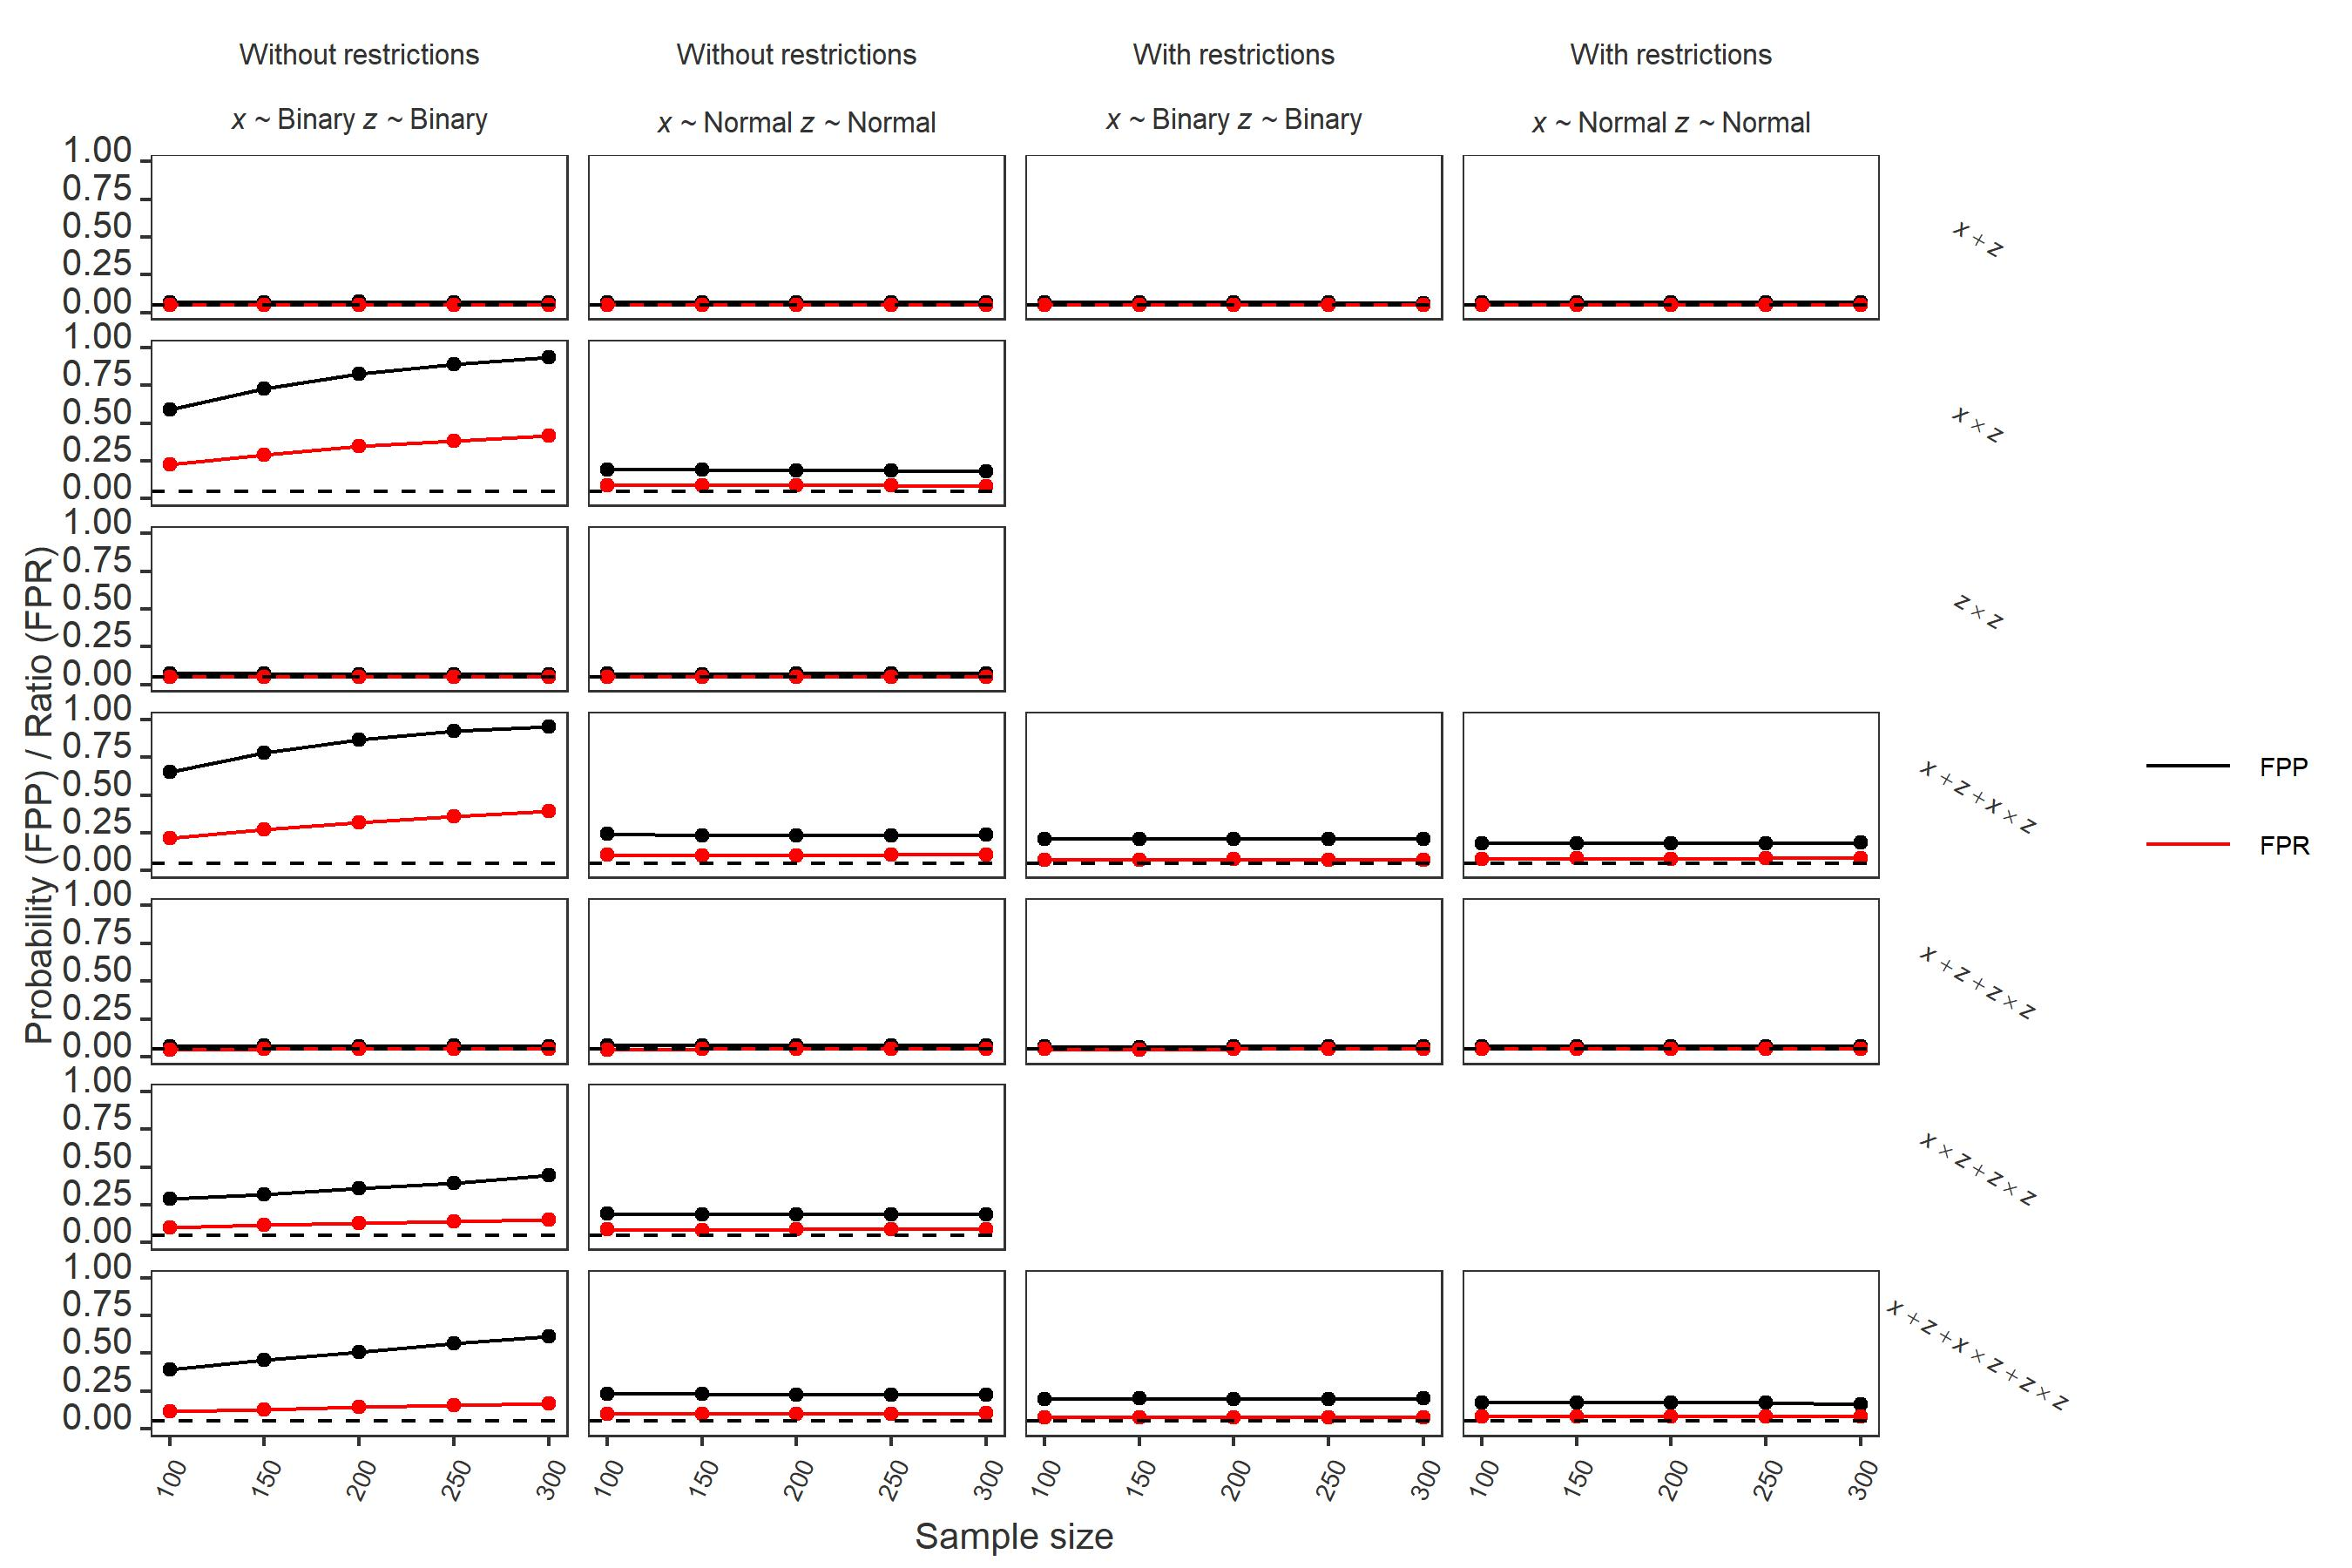
\includegraphics[width=0.9\textwidth]{R/Analysis/Result/Figures/Figure1D.jpeg}
\centering
\caption{The effect of increasing sample size on the FPP and FPR. Black denotes the FPP and red denotes FPR. The description of the figure is otherwise the same as for Figure 1.}
\label{fig:mainfigure}
\end{figure}

\subsection{Correlation}
A higher correlation between the dependent variable and the covariates also increased the FPP and FPR for some model sets. In general, the FPP and FPR were higher as the correlation increased and the main effects did not follow the interactions. The model sets with the highest increase for both the FPP and FPR were the sets that contained HCI. The effect was most pronounced when the variable of interest and covariates were binary (as can be seen in Figure S2). The increase in the FPP for these sets was between 15\% and 23\% when the correlation increased from r=0.2 to r=0.3. When the correlation increased from r=0.3 to r=0.4, the FPP increased only for those sets where there was still room for an increase, since a high number of the sets already had the FPP close to 100\% (see Figure S2). The increase in correlation also affected the FPR for the same sets increasing it to as high as 10\%. When the main effects were present, the FPP and FPR seemed to have a much lower increase (See Figure S2).

% discussion section
\section{Discussion}

- Background and research question: moving towards higher reproducibility by fighting false positive results. One of the ways researchers have moved to lower this is with open science and preregistration. 
- troubles in paradise: is prereg enough?
With literature showing that even with just running one model can increase the false positive preregistration might not be enough (REF). 
With simulations showing an increase in the FPP even just labeling the research as exploitative might be a bad idea \citep{Simmons2011}. 
Using a simulation, we looked at how FPP and FPR were affected by different flexibilities. More precisely, we looked into the flexibilities; constructing a model set with several covariates, using multiple outlier criteria, and collecting different dependent variables. We also looked on how the precision of the estimates (a bigger sample) and the correlations between the dependent variable and the covariates affected the ability to find a significant effect both when the study would be labeled as exploratory but also under the criteria of preregistration. 


- our RQ: analyze FPP AND FPR to understand the risk of false positive findings even under prereg and labelling as "exploratory"
- How did we answer this: short recap on sim setup
- main findings:
	- Preregistration is not enough to lower the FPR to 5\%  in some cases. This happens when main effects are not included and the covariates are dummy coded. In this case the FPR can get as high as ...\%, meaning that when the research just run random model from a given set there is already a false positive rate at ...\%. This happens due to the fact that the interaction effect captures the true effect that would have been from the main effect. So even though some literature still suggest this when the reasoning is just theory based, there seems to be no good reason for this as long as the covariates are dummy coded. This also means that the FPR falls as soon as the variable is effects coded, but it still due not drop down to an FPR at 5\%. The only way to overcome this issue is to always include the main effect as soon as interactions are of interest. However, even in the sets that that includeds the main effects and interactions the FPR will still be slightly higher than 5\%. This is simple due to the fact that multiple test's are been looked at at the same time. A simple solution to overcome this issue is to correct the p-values for this multiple comparison, such as using Bonferroni correction (REF).
    - we need solid statistics (always have main effects) and correcting p-values 
	- exploratory analyses still gives issues - p-values have little to no meaning
	- sample size is not the solution and can even bring problems
- recommendations
- additional contribution to model selection and machine learning research: calculate how big the model set is depending on which part in the set one is looking at - if not interested in one specific the sets Ma, CCI and Ma+ CCI are the sets to look at

Note: make calculations in appendix


Guidelines for researchers 
\begin{itemize}
\item Follow the principals and guidelines of open science.
Researchers should follow the guidelines already developed (Nosek et al., 2015) to get the FPP to the expected 5\%.
\item Use effects coding and not dummy coding
If there, for some reason, should be a reason not to include main effects when doing interactions. This lowers both the FPP and FPR for sets that include HCI and there is no main effect present.
\item Use Bonferroni corrections when looking at interactions. When running regressions (or ANOVA) with interaction effects a Bonferroni correction should be used. If this is not being done the FPR will be higher than 5\%, and therefore the FPP would also be higher than 5\%.
\end{itemize}


Guidelines for reviewer and editors
\begin{itemize}
\item Look for correction of p-values
If multiple comparisons are being made or interaction effects are used, there should be a correction of the p-values
\item Demand main effects follow interaction effects
If the main effect is not included when interaction effects are investigated there should be a thorough explanation of why this is the case.
\end{itemize}
 


% author contributions
\section{Author contributions}
JDC and JLO developed the study concept. JDC and SP performed the analyses. JDC, SP, CJL, and JLO wrote the manuscript. 

% data and code
\section{Data availability}
All code for simulation and figures in the paper can be found at \url{https://osf.io/2c5zw/}.

% reference list
\bibliographystyle{apalike}
\bibliography{references.bib}
\clearpage

% appendix
 \section{Appendix} 

\setcounter{table}{0}
\setcounter{figure}{0}
\renewcommand{\thetable}{A\arabic{table}}
\renewcommand{\thefigure}{A\arabic{figure}}

\subsection{Binomial coefficient}
\label{binomial}
In the following sections we present the equations and methods used for calculating the model set sizes for different model sets under different conditions. To calculate the size of the different model sets, we use binomial coefficients to calculate the number of possible combinations. The general form of the binomial coefficient is written as
\[\left( \begin{array}{c}
n \\ 
k \end{array}
\right)=\frac{n!}{k!\left(n-k\right)!}\] 
where $n$ is the number of elements which in our case is the number of covariates ($z$) that we want to include, and $k$ is the number of elements taken out. $!$ is the factorial operator, so $n!=n\times \left(n-1\right)\times \left(n-2\right)\times \left(n-3\right)\times \dots \times 3\times 2\times 1$. The binomial coefficient therefore gives us the number of ways that $k$ elements can be chosen from a set of size $n$. One rule that has been repeatedly used is that we can rewrite the sum of binomial coefficients excluding the empty set i.e., not including $i=0$, as 
\[\sum^n_{i=1}{\left( \begin{array}{c}
n \\ 
i \end{array}
\right)}=2^n-1\] 
\\
If we include the empty set this becomes
\[\sum^n_{i=0}{\left( \begin{array}{c}
n \\ 
i \end{array}
\right)}=2^n\] 
\\
When calculating the size of each model set, we consider two different cases; a case without restrictions where we allow interactions without the corresponding main effects, and a case with restrictions where main effects always follow interactions. This means that the second case will be a subset of the first case. \\

% section
\subsection{Model sets without restrictions}
\label{witout_res}
\subsubsection{Set $x + z$}
To calculate the size of the sets, we use the binomial coefficient. The set $x + z$ contains all the combinations that can be made by the covariates $z$ including the model where there is only the variable of interest $x$. Based on the previous terminology the model containing only the variable of interest is therefore the empty set and the binomial coefficient therefore computes how many combinations there are. Let us denote the number of covariates $n$. If we, for example, have three covariates ($n=3$), then the number of combinations where all three covariates are present can be written using the binomial coefficient as
\[\left( \begin{array}{c}
3 \\ 
3 \end{array}
\right)=\frac{3!}{3!\left(3-3\right)!}=1\]
If only two covariates are included in the model from the set of three possible covariates, then the number of combinations becomes 
\[\left( \begin{array}{c}
3 \\ 
2 \end{array}
\right)=\frac{3!}{2!\left(3-2\right)!}=3\] 
And the same if only one covariate is present
\[\left( \begin{array}{c}
3 \\ 
1 \end{array}
\right)=\frac{3!}{1!\left(3-1\right)!}=3\] 
Finally, where no covariates are present, the number of possible combinations is computed as follows
\[\left( \begin{array}{c}
3 \\ 
0 \end{array}
\right)=\frac{3!}{0!\left(3-0\right)!}=1\] 
The total number of models in this set will then be the sum of all these


\[\#\ of\ models\ in\ x + z = \left( \begin{array}{c}
3 \\ 
3 \end{array}
\right)+\left( \begin{array}{c}
3 \\ 
2 \end{array}
\right)+\left( \begin{array}{c}
3 \\ 
1 \end{array}
\right)+\left( \begin{array}{c}
3 \\ 
0 \end{array}
\right)=\sum^3_{i=0}{\left( \begin{array}{c}
3 \\ 
i \end{array}
\right)}\] 
Using the rule for adding binomial coefficients, we can rewrite this into
\[\#\ of\ models\ in\ x + z = \sum^3_{i=0}{\left( \begin{array}{c}
3 \\ 
i \end{array}
\right)}=\left(2^3\right)=8\] 
We can generalize this to the case with $n$ covariates  as follows 
\[\#\ of\ models\ in\ x + z\sum^n_{i=0}{\left( \begin{array}{c}
n \\ 
i \end{array}
\right)}=\left(2^n\right)\] 

\subsubsection{Formally Written} Let $Z$ be the set of covariates 
\[Z=\{\left.z_1,z_2,..,z_n\right.\}\] 
\[\left|Z\right|=n\] 


\noindent The $x + z$ set is then the power set of \emph{Z} 
\[x + z = \{\left.S:S\subseteq Z\right.\}\] 

Each element $S\in x + z$ is a set of the covariates e.g., $S=\left.z_3,z_7\right.$, or any combination of the covariates, including the empty set. This is just the power set of $Z$ and the size of the set can be written as
\[\left|x + z\right|=|\mathcal{P}\left(Z\right)|=2^n\] 
% section
\subsubsection{Set $x \times z$}
The same line of reasoning goes for the $x \times z$ set as for $x + z$ set and we therefore only write it formally. Here, we need to calculate the number of possible interactions between the variable of interest and covariates. This set will therefore have the same size as the $x + z$ set, as there are as many covariates as there are two-way combinations between the variable of interest and covariates excluding the empty set.

\[I_h(Z)=\left.\left\{\{x,z_i\}\right.:z_i\in Z\right.\}\] 
\[x \times z=\left.\{T:T\subseteq I_h\left(Z\right),T\neq \textrm{\O}\right.\}\] 
The total number of models in this set is the power set excluding the empty set
\[\left|x \times z\right|\boldsymbol{=}2^n-1\] 

% section
\subsubsection{Set $z \times z$}
The $z \times z$ set contains all combinations of all two-way interactions between the covariates. We first calculate the number of two-way interactions between the covariates and then calculate the number of combinations of these interactions. In the example were $n=3$, the number of two-way interactions is as follows
\[\#\ of\ two-way\ interactions=\left( \begin{array}{c}
3 \\ 
2 \end{array}
\right)=\frac{3!}{2!\left(3-2\right)!}=3\] 
We can then compute the number of combinations of two-way interaction effects using the same method as above 

\noindent 
\[\#\ of\ models\ in\ z \times z=\left( \begin{array}{c}
3 \\ 
3 \end{array}
\right)+\left( \begin{array}{c}
3 \\ 
2 \end{array}
\right)+\left( \begin{array}{c}
3 \\ 
1 \end{array}
\right)=\sum^3_{i=1}{\left( \begin{array}{c}
3 \\ 
i \end{array}
\right)}=7\] 
In general, we can define the number of two-way interactions $h$ that can be generated with $n$ covariates as
\[h=\left( \begin{array}{c}
n \\ 
2 \end{array}
\right)=n(n-1)/2\] 
and the general term for the total number of models in $z \times z$ as
\[\#\ of\ models\ in\ z \times z=\sum^{n(n-1)/2}_{i=1}{\left( \begin{array}{c}
n(n-1)/2 \\ 
i \end{array}
\right)}=(2^{n(n-1)/2}-1)=2^h-1\] 


\subsubsection{Formally written}
Let $Z$ be a set of covariates 
$Z=\{z_1,z_2,..,z_n\}$
\[I_k\left(Z\right)=\{\{\left.\left.z_i,z_j\right.\}:z_i\in Z,z_j\in Z,z_i\neq z_j\right.\}\] 
\[\left|I_k\left(Z\right)\right|=\left( \begin{array}{c}
n \\ 
2 \end{array}
\right)=\frac{n\left(n-1\right)\left(n-2\right)!}{\left(n-2\right)!}\frac{1}{2}=n(n-1)/2\] 
The set of all combinations of two-way interactions between the covariates is then all the subsets of $I_k\left(Z\right)$ excluding the empty set
\[P\left(I_k\left(Z\right)\right)=\{\left.J:J\subseteq I_k\left(Z\right),J\neq \textrm{\O}\right.\}\] 
\[\left|z \times z\right|=\left|P\left(I_k\left(Z\right)\right)\right|=2^{\left|I_k\left(Z\right)\right|}-1=2^{n(n-1)/2}-1\] 
defining 
\[h=\left( \begin{array}{c}
n \\ 
2 \end{array}
\right)=n(n-1)/2\] \\
We can write the number of models in $z \times z$ as
\[\left|z \times z\right|=2^h-1\] \\

% section
\subsubsection{Full model set}
For the following sets: $x + z + x \times z$ , $x + z + z \times z$, and $x + z + x \times z$ + $z \times z$, the equations follow directly from the previous equations as these sets are the products of the previously calculated sets. 

\[\# of\ models\ in\ x + z =\left(2^n\right)\] 
\[\# of\ models\ in\ x \times z=\left(2^n-1\right)\] 
\[\# of\ models\ in\ z \times z=\left(2^h-1\right)\] 
\[\# of\ models\ in\ x + z + x \times z={\left(2^n-1\right)}^2\] 
\[\# of\ models\ in\ x + z+z \times z=\left(2^n-1\right)\left(2^h-1\right)\] 
\[\# of\ models\ in\ x + z + x \times z+z \times z={\left(2^n-1\right)}^2\left(2^h-1\right)\] 
So the total number of models including all sets then becomes
\begin{equation*}
\begin{aligned}
total\ \# \ of\ models=\\
& \underbrace{\left(2^n\right)}_{x + z}+\underbrace{\left(2^n-1\right)}_{x \times z}+\underbrace{\left(2^h-1\right)}_{z \times z}+\\
&\underbrace{{\left(2^n-1\right)}^2}_{x + z + x \times z}+\underbrace{\left(2^n-1\right)\left(2^h-1\right)}_{x \times z+z \times z}+\underbrace{\left(2^n-1\right)\left(2^h-1\right)}_{x + z+z \times z}+\\
&\underbrace{{\left(2^n-1\right)}^2\left(2^h-1\right)}_{x + z + x \times z+z \times z} 
\end{aligned}
\end{equation*}

% For the case where $n=2$, (as in Table \ref{modelsets2.1} under "Models without restrictions" of the main paper), this gives us
%\[h=\left( \begin{array}{c}
%2 \\ 
%2 \end{array}
%\right)=1\] 
%$total \ \#\ of\ models=\left(2^2\right)+\left(2^2-1\right)+\left(2^1-1\right)+{\left(2^2-1\right)}^2+2\left(2^2-1\right)\left(2^1-1\right)+{\left(2^2-1\right)}^2\left(2^1-1\right)=32$ 

% section
\subsection{Model sets with restrictions}
\label{with_res}
In the case with restrictions, we enforce that every time there is an interaction effect, the corresponding main effects are included in the model as in the model below:
\[y=x_1+z_1+x_1z_1\] 

In the previous equation, we have an interaction between our variable of interest $x_1$ and a covariate $z_1$. Therefore, the two corresponding main effects also enter the model. This restriction does not change how we calculate the set size of the $x + z$ set as there are no interactions in it. On the other hand,  the restriction implies that the sets $x \times z$ and $z \times z$ are empty sets as the models in these sets never have main effects following interactions. The first set we then need to calculate is then the set $x + z + x \times z$.

% section
\subsubsection{Set $x + z + x \times z$}
For the sake of simplicity, we begin with the case where $n=3$. The models in this set can be seen in Table \ref{tab:appmodel2}. Here the models are split into three different parts. These are split such that $x + z + x \times z$(1), $x + z + x \times z$(2), and $x + z + x \times z$(3) contain all the models where there are one, two, or three covariates, respectively.\\

%\begin{table}[ht!]
%\caption{}
%\caption*{Overview of the models in the $x + z + x \times z$ set when there are three %covariates and one dependent variable}
%\label{tab:appmodel1}
%\centering
%\begin{tabular}{cc}
%\toprule
%Model set & Models \\ 
%\midrule
%\multirow{19}{*}{$x + z + x \times z$} & $y=x_1+z_1+x_1z_1$\\ &  $y=x_1+z_2+x_1z_2$\\ &  $y=x_1+z_3+x_1z_3$\\ & $y=x_1+z_1+z_2+x_1z_1$\\ & $y=x_1+z_1+z_3+x_1z_1$\\ & $y=x_1+z_3+z_1+x_1z_3$\\ & $y=x_1+z_3+z_2+x_1z_3$\\ & $y=x_1+z_2+z_1+x_1z_2$\\ & $y=x_1+z_2+z_3+x_1z_2$\\ & $y=x_1+z_1+z_2+z_3+x_1z_1$\\ & $y=x_1+z_1+z_2+z_3+x_1z_2$\\ & $y=x_1+z_1+z_2+z_3+x_1z_3$\\ & $y=x_1+z_1+z_2+x_1z_1+x_1z_2$\\ & $y=x_1+z_1+z_3+x_1z_1+x_1z_3$\\ & $y=x_1+z_1+z_2+x_1z_3+x_1z_2$\\ & $y=x_1+z_1+z_2+z_3+x_1z_1+x_1z_2$\\ & $y=x_1+z_1+z_2+z_3+x_1z_1+x_1z_3$\\ & $y=x_1+z_1+z_2+z_3+x_1z_3+x_1z_2$\\ & $y=x_1+z_1+z_2+z_3+x_1z_1+x_1z_2+x_1z_3$\\  
%\bottomrule
%\end{tabular}
%\end{table}

\begin{table}[ht!]
\caption{Example of division of the $x + z + x \times z$ set into three subsets when there are three covariates and one dependent variable. $x + z + x \times z$(1) contains all the models with one covariate as main effect, $x + z + x \times z$(2) all the models with two covariates, and $x + z + x \times z$(3) all the models with three covariates}
\centering\label{tab:appmodel2}
\begin{tabular}{lc}  
\toprule
Set & Models \\
\midrule
\multirow{3}{*}{$x + z + x \times z$(1)} & $y=x_1+z_1+x_1z_1$\\ & $y=x_1+z_2+x_1z_2$\\ & $y=x_1+z_3+x_1z_3$\\ & \\ 
\multirow{9}{*}{$x + z + x \times z$(2)} & $y=x_1+z_1$$+z_2+x_1z_1$\\ & $y=x_1+z_1+z_3+x_1z_1$\\ & $y=x_1+z_3+z_1+x_1z_3$\\ & $y=x_1+z_3+z_2+x_1z_3$\\ & $y=x_1+z_2+z_1+x_1z_2$\\ & $y=x_1+z_2+z_3+x_1z_2$\\ & $y=x_1+z_1+z_2+x_1z_1+x_1z_2$\\ & $y=x_1+z_1+z_3+x_1z_1+x_1z_3$\\ & $y=x_1+z_1+z_2+x_1z_3+x_1z_2$\\  & \\  
\multirow{7}{*}{$x + z + x \times z$(3)} & $y=x_1+z_1+z_2+z_3+x_1z_1$\\ & $y=x_1+z_1+z_2+z_3+x_1z_2$\\ & $y=x_1+z_1+z_2+z_3+x_1z_3$\\ & $y=x_1+z_1+z_2+z_3+x_1z_1+x_1z_2$\\ & $y=x_1+z_1+z_2+z_3+x_1z_1+x_1z_3$\\ & $y=x_1+z_1+z_2+z_3+x_1z_3+x_1z_2$\\ & $y=x_1+z_1+z_2+z_3+x_1z_1+x_1z_2+x_1z_3$\\  
\bottomrule
\end{tabular}
\end{table}

To calculate the size of each of these sets separately, we only need to focus on the number of covariates that enter the model, as per assumption the variable of interest $x_1$ is always present. Let us start with the $x + z + x \times z$(1) set. In this set, there can only be one covariate present at the time; there are therefore three combinations, which can be written as $\binom{3}{1}$. In this set, since there is only one covariate, there is only one interaction effect containing that same covariate. As no other combinations can be made, this corresponds to $\binom{1}{1}$. Using the same shorthand notation with the binomial coefficient as above, we can write the number of models in the $x + z + x \times z$(1) set as
\[\#\ of\ models\ in\ x + z + x \times z\textit{(1)}\ =\left( \begin{array}{c}
1 \\ 
1 \end{array}
\right)\left( \begin{array}{c}
3 \\ 
1 \end{array}
\right)=\sum^1_{i=1}{\left( \begin{array}{c}
1 \\ 
i \end{array}
\right)}\left( \begin{array}{c}
3 \\ 
1 \end{array}
\right)=\left(2^1-1\right)\left( \begin{array}{c}
3 \\ 
1 \end{array}
\right)=3\] 
Using this notation is useful when we later have to combine the three sets of $x + z + x \times z$ into one to calculate the total number of models in $x + z + x \times z$.

For the $x + z + x \times z$(2) set, we first need to calculate the number of combinations for the main effect that can be made when there are two covariates present at all times and that is $\binom{3}{2}$. Next we need to calculate the number of combinations of interactions that can be present. As we have two covariates present all the time, these are the ones that can be used in the interaction effects. Since the covariates interact with $x_1$, there can either be one or two interaction effects present. Hence, we have $\binom{2}{1}$ and $\binom{2}{2}$ combinations of the interaction effects possible. Combining the number of covariates with the number of possible interactions we get

\begin{equation*}
\begin{aligned}
\#\ of\ models\ in\ x + z +x \times z\textit{(2)}=\\
& \left( \begin{array}{c}
2 \\ 
1 \end{array}
\right)\left( \begin{array}{c}
3 \\ 
2 \end{array}
\right)+\left( \begin{array}{c}
2 \\ 
2 \end{array}
\right)\left( \begin{array}{c}
3 \\ 
2 \end{array}
\right)=\\
&\sum^2_{i=1}{\left( \begin{array}{c}
2 \\ 
i \end{array}
\right)}\left( \begin{array}{c}
3 \\ 
2 \end{array}
\right)=\left(2^2-1\right)\left( \begin{array}{c}
3 \\ 
2 \end{array}
\right)=9

\end{aligned}
\end{equation*}

The same reasoning goes for the $x + z + x \times z$(3) set; the only difference here is that we have one more covariate. So if we write the combinations that are possible with three covariates in the same way as before, we get
\begin{equation*}
\begin{aligned}
\#\ of\ models\ in\ x + z + x \times z\textit{(3)}=\\
&\left( \begin{array}{c}
3 \\ 
1 \end{array}
\right)\left( \begin{array}{c}
3 \\ 
3 \end{array}
\right)+\left( \begin{array}{c}
3 \\ 
2 \end{array}
\right)\left( \begin{array}{c}
3 \\ 
3 \end{array}
\right)+\left( \begin{array}{c}
3 \\ 
3 \end{array}
\right)\left( \begin{array}{c}
3 \\ 
3 \end{array}
\right)= \\
&\sum^3_{i=1}{\left( \begin{array}{c}
2 \\ 
i \end{array}
\right)}\left( \begin{array}{c}
3 \\ 
2 \end{array}
\right)= \\
&\left(2^3-1\right)\left( \begin{array}{c}
3 \\ 
3 \end{array}
\right)=7
\end{aligned}
\end{equation*}
We can then sum all three sets that is, $x + z + x \times z$(1), $x + z + x \times z$(2), and $x + z + x \times z$(3), to get the size of the $x + z + x \times z$ set
\[\#\ of\ models\ in\ x + z + x \times z=\sum^3_{k=1}{(2^k-1)\left( \begin{array}{c}
3 \\ 
k \end{array}
\right)}\]where $k$ is the number of covariates that enter as main effects, meaning it is an indicator for $x + z + x \times z$(1), $x + z + x \times z$(2) and $x + z + x \times z$(3). For the case with $n$ covariates, this becomes
\[\#\ of\ models\ in\ x + z + x \times z=\sum^n_{k=1}{(2^k-1)\left( \begin{array}{c}
n \\ 
k \end{array}
\right)}\] 
\subsubsection{Formally written}
Let $Z$ be a set of covariates 
\[Z=\{\left.z_1,z_2,\dots ,z_n\right.\}\] \[|Z|=n\] 

Let $J$ be a set of indicators of how many covariates enter the model set as main effects
\[J=\{\left.1,2,3,4,\dots ,n\right.\}\] 
Let $L$ be a subset of $Z$ of size $k$
\[L=\{\left.S:S\subset Z,\left|S\right|=k,k\in J\right.\}\] 
The number of interactions that can be made between a covariate and the variable of interest for a given $k$ is then
\[I_h\left(Z\right)=\{\{\left.\left.z_i,x_1\right.\}:z_i\in L\right.\}\] 
\[\left|I_h\left(Z\right)\right|=k\] 

For each $k$, the number of interactions is just the power set of $Z$ excluding the empty set
\[\left|\mathcal{P}\left(I_h\left(Z\right):I_h\left(Z\right)\neq \textrm{\O}\right)\right|=2^k-1\] 

For each $k$, there is $\left( \begin{array}{c}
n \\ 
k \end{array}
\right)$ combinations of interactions that can be present with the number of covariates $k$. To get the full set, we need to sum over these combinations from $k=1$ to $n$ (with $k=0$ it would not be possible to make any interactions so this one is excluded).
\[\left|x + z + x \times z\right|=\sum^n_{k=1}{\left( \begin{array}{c}
n \\ 
k \end{array}
\right)\left(2^k-1\right)}\] 

% section
\subsubsection{Set $x + z + z \times z$}
Here we can use the same line of reasoning as for the $x + z + x \times z$ set. Let us begin by examining the case where $n=3$ and then develop a more general notion. To make it easier to understand how to calculate the set size, we split this set into subsets as we did above for the $x + z + x \times z$ set. This example can be seen in Table \ref{tab:appmodel4}. 

\begin{table}
\centering
\caption{Division of the $x + z + z \times z$ set into two subsets when there are three covariates and one dependent variable. $x + z + z \times z$(2) contains all the models with two covariates as main effects, and $x + z + z \times z$(3) all the models with three covariates. $x + z + z \times z$(1) is an empty set since at least two covariates are necessary to make an interaction.}
\label{tab:appmodel4}
\begin{tabular}{lc} 
\toprule
Set & Models \\ 
\midrule
\multirow{3}{*}{$x + z + z \times z$(2)} & $y=x_1+z_1+z_2+z_1z_2$\\ & $y=x_1+z_1+z_3+z_1z_3$\\ & $y=x_1+z_2+z_3+z_2z_3$\\ &  \\  
\multirow{7}{*}{$x + z + z \times z$(3)} & $y=x_1+z_1+z_2+z_3+z_1z_2$\\ & $y=x_1+z_1+z_3+z_2+z_1z_3$\\ & $y=x_1+z_2+z_3+z_1+z_2z_3$\\ & $y=x_1+z_1+z_2+z_3+z_1z_2+z_1z_3$\\ & $y=x_1+z_1+z_3+z_2+z_1z_3+z_2z_3$\\ & $y=x_1+z_2+z_3+z_1+z_1z_2+z_2z_3$\\ & $y=x_1+z_1+z_2+z_3+z_1z_2+z_2z_3+z_1z_3$\\ 
\bottomrule
\end{tabular}
\end{table}

A model must always include at least two covariates to fulfil the restriction that main effects follow interactions effects. Therefore, we can divide the $x + z + z \times z$ set into two subsets; the first subset has two covariates present as main effects and the second subset has three covariates present as main effects. The first set, $x + z + z \times z$(2), is the number of combinations that can be made from two out of three covariates, meaning $\binom{3}{2}$, multiplied with the combinations of the two covariates that are included, meaning $\binom{2}{2}$.
\[\#\ of\ models\ in\ x + z + z \times z\textit{(2)} =\left( \begin{array}{c}
3 \\ 
2 \end{array}
\right)\left( \begin{array}{c}
2 \\ 
2 \end{array}
\right)=3\] 
For the second subset, $x + z + z \times z$(3), the first term is the number of combinations that can be made with three covariates so this is $\binom{3}{3}$. We then have to calculate the number of interactions that can be made with the three included covariates. To do that, first we need to calculate the number of two-way interactions that can be made with three covariates and this is $\binom{3}{2}=3$. The total number of models in the set is then the sum of the number of combinations
\[\#\ of\ models\ in\ x + z + z \times z\textit{(3)}=\left( \begin{array}{c}
3 \\ 
3 \end{array}
\right)\left(\left( \begin{array}{c}
3 \\ 
1 \end{array}
\right)+\left( \begin{array}{c}
3 \\ 
2 \end{array}
\right)+\left( \begin{array}{c}
3 \\ 
3 \end{array}
\right)\right)=\left( \begin{array}{c}
3 \\ 
3 \end{array}
\right)\sum^3_{i=1}{\left( \begin{array}{c}
3 \\ 
i \end{array}
\right)}\] 
However, it is only in this example that we sum to $n=3$. In general, this will be the number of pairs that can be made in this subset. The number of pairs can be written as $\left( \begin{array}{c}
n \\ 
2 \end{array}
\right)=\frac{n\left(n-1\right)}{2}$. This then becomes
\[\#\ of\ models\ in\ x + z + z \times z\textit{(3)}=\left( \begin{array}{c}
3 \\ 
3 \end{array}
\right)\sum^3_{i=1}{\left( \begin{array}{c}
3 \\ 
i \end{array}
\right)}=\left( \begin{array}{c}
3 \\ 
3 \end{array}
\right)\sum^{\frac{3\left(3-1\right)}{2}}_{i=1}{\left( \begin{array}{c}
\frac{3\left(3-1\right)}{2} \\ 
i \end{array}
\right)}=\left( \begin{array}{c}
3 \\ 
3 \end{array}
\right)\left(2^{\frac{3\left(3-1\right)}{2}}-1\right)\] 
We can write the first subset in the same way
\[\#\ of\ models\ in\ x + z + z \times z(2)=\left( \begin{array}{c}
3 \\ 
2 \end{array}
\right)=\left( \begin{array}{c}
3 \\ 
2 \end{array}
\right)\left(2^{\frac{2\left(2-1\right)}{2}}-1\right)\] 
Now we just add these two subsets up
\[\#\ of\ models\ in\ x + z + z \times z=\left( \begin{array}{c}
3 \\ 
2 \end{array}
\right)\left(2^{\frac{2\left(2-1\right)}{2}}-1\right)+\left( \begin{array}{c}
3 \\ 
3 \end{array}
\right)\left(2^{\frac{3\left(3-1\right)}{2}}-1\right)=\sum^3_{j=2}{\left( \begin{array}{c}
3 \\ 
j \end{array}
\right)\left(2^{\frac{j\left(j-1\right)}{2}}-1\right)}\] 
We can then generalize this case for $n$ covariates
\[\#\ of\ models\ in\ x + z+z \times z=\sum^n_{j=2}{\left( \begin{array}{c}
n \\ 
j \end{array}
\right)\left(2^{\frac{j\left(j-1\right)}{2}}-1\right)}\] 

\subsubsection{Formally written}
Let $Z$ be a set of covariates 
\[Z=\{\left.z_1,z_2,\dots ,z_n\right.\}\] 
\[|Z|=n\] 
Let $k$ be an indicator of how many covariates are included. Since we are using interactions, $k$ must begin at two. Let $T$ be a set of indicators of the number of covariates beginning at two
\[T=\{\left.2,3,4,\dots ,n\right.\}\] 
Let $L$ be a subset of $Z$ of size $k$
\[L=\{\left.S:S\subset Z,\left|S\right|=k,k\in T\right.\}\] 

The number of interactions that can be made for a given $k$ is then
\[I_k\left(Z\right)=\{\left\{\left.z_i,z_j\right\}:z_i\in L,z_j\in L,z_i\neq z_j\right.\}\] 
For a given $k$, the number of two-way interactions that can be made is then
\[\left|I_k\left(Z\right)\right|=\left( \begin{array}{c}
k \\ 
2 \end{array}
\right)=\frac{k!}{2!\left(k-2\right)!}=\frac{k\left(k-1\right)\left(k-2\right)!}{\left(k-2\right)!}\frac{1}{2}=\frac{k\left(k-1\right)}{2}\] 
We then need the combinations of all the two-way interactions. For all $k$, we can take the power set of $I_k\left(H\right)$ excluding the empty set
\[P\left(I_k\left(Z\right)\right)=\{\left.T:T\subset I_k\left(Z\right),T\neq \textrm{\O}\right.\}\] 
\[\left|P\left(I_k\left(Z\right)\right)\right|=2^{\left|I_k\left(Z\right)\right|}-1=2^{\frac{k\left(k-1\right)}{2}}-1\] 
With $n$ covariates, there exist $\left( \begin{array}{c}
n \\ 
k \end{array}
\right)$ subsets of size $k$. To get the $x + z + z \times z$ set, we need to sum over the number of covariates $k$ starting from $k=2$
\[\left|x + z+z \times z\right|=\sum^n_{k=2}{\left( \begin{array}{c}
n \\ 
k \end{array}
\right)}\left(2^{\frac{k\left(k-1\right)}{2}}-1\right)\ \] 

% section
\subsubsection{Set $x + z + x \times z$ + $z \times z$}
This set is the product of the $x + z + x \times z$ and $x + z + z \times z$ sets, but without including the main effect twice. Hence, the set consists of the combinations that can be made between the variable of interest and the covariates and between the covariates alone. We can therefore write 
\[\#\ of\ models\ in\ x + z + x \times z+\ z \times z=\sum^n_{k=2}{\left( \begin{array}{c}
n \\ 
k \end{array}
\right)\left(2^k-1\right)\left(2^{\frac{k\left(k-1\right)}{2}}-1\right)}\] 
\subsubsection{Formally written}
The design of the subsets is the same as earlier and we need to take the product of
$P\left(I_k\left(Z\right)\right)$ and $P\left(I_h\left(Z\right)\right)$, as defined above, and sum over $k$ beginning at two.
For $n$ covariates, there exists $\left( \begin{array}{c}
n \\ 
k \end{array}
\right)$ subsets of size $k$. We then need to sum the subsets as follows
\[|x + z + x \times z+z \times z|=\sum^n_{k=2}{\left( \begin{array}{c}
n \\ 
k \end{array}
\right)\left(2^k-1\right)\left(2^{\frac{k\left(k-1\right)}{2}}-1\right)}\] 

% section
\subsection{Full model set with restrictions}
We now have the full set of models in the $n$ covariate case written as
\begin{equation} 
\begin{aligned}
\#\ models={} & \underbrace{\left(2^n\right)}_{x + z}+\underbrace{\sum^n_{k=1}{\left(2^k-1\right)\binom{n}{k}}}_{x + z + x \times z} + \\ 
& \underbrace{\sum^n_{k=2}{\binom{n}{j}\left(2^{\frac{k\left(k-1\right)}{2}}-1\right)}}_{x + z + z \times z} + \\
& \underbrace{\sum^n_{k=2}{\binom{n}{k}\left(2^k-1\right)\left(2^{\frac{k\left(k-1\right)}{2}}-1\right)}}_{x + z + x \times z + z \times z}\ \  
\end{aligned}
\end{equation} 

\clearpage
% section
%\subsection{Number of Models}
%In the case without restrictions where we allow interactions without including the corresponding main effects, the total number of models per each set given the number of covariates can be seen in Table \ref{FullModel} under "Without restrictions" in the main paper. For the case with restrictions, the total number of models per each set can be found in either Table \ref{FullModel} in the main part of the manuscript under "With restrictions". 


%\section{Model set for machine learning}
%When researchers are not interested in one specific variable but rather the overall prediction of a given model, such as in machine learning, the same terminology for the sets as used previously can be used to calculate the size of the model sets. 
%As is the case with hypothesis testing, researchers can either demand that main effects are always present when having interactions or they can relax this restriction. \\

%\subsection{When no restrictions are in place}
%In this case, there are three possible sets: $z$, $z \times z$, and $ z + z \times z$. In this case there is no variable that needs to be present all the time as earlier ($x_1$). The calculations of the model set sizes are nevertheless similar to the example with two covariates with no restrictions (see Supplementary Material Case 1 - No Restrictions), and this can be seen in Table \ref{tab:appmodel5} and equation \ref{eq:model1}, \ref{eq:model2} and \ref{eq:model3}.  

%\begin{table}
%\caption{Models for the set $z$, $z \times z$ and $ z + z \times z$ that can be made with two covariates when there is no specific variable of interest. $c$ is a constant, whereas $z_1$ and $z_2$ are covariates}
%\label{tab:appmodel5}
%\centering
%\begin{tabular}{lc} 
%\toprule
%Set & Models \\ 
%\midrule
%\multirow{4}{*}{z} & $y=c$\\ & $y=c + z_1$\\ & $y=c + z_2$\\ & $y=c + z_1 + z_2$\\ &  \\  
%\multirow{1}{*}{$z \times z$} & $y=c + z_1z_2$\\  & \\ 
%\multirow{3}{*}{$x + z + z \times z$}  & $y=c + z_1 + z_1z_2$\\ & $y=c + z_2 + z_1z_2$\\ & $y=c + z_1 + z_2 + z_1z_2$\\ &  \\  
%\bottomrule
%\end{tabular}
%\end{table}

%The calculation for the set size is done as in "Case 1 - No Restrictions"

%\begin{equation}
%\label{eq:model1}
%  \# of\ models\ in\  z\left(2^n\right)
%\end{equation}
%\begin{equation}
%\label{eq:model2}
%  \# of\ models\ in\ z \times z=\left(2^h-1\right)
%\end{equation}
%\begin{equation}
%\label{eq:model3}
%  # of models\ in\ z+z \times z=\left(2^n-1\right)\left(2^h-1\right)
%\end{equation}

%where $h=\left( \begin{array}{c}
%n \\ 
%2 \end{array}
%\right)$. 

%The total number of models given the different number of covariates can be seen in Table \ref{tab:appmodel6}. These calculations apply only when allowing for two-way interactions, but this framework can easily be expanded to include higher order interactions. \\

%% latex table generated in R 4.0.0 by xtable 1.8-4 package
% Wed Dec 30 11:47:49 2020
\begin{table}[!h]
\centering
\caption{} 
\begin{tabular}{rrrrr}
  \hline
Number of covariates & ME & CCI & ME+CCI & Number of models \\ 
  \hline
2 & 4 & 1 & 3 & 8 \\ 
  3 & 8 & 4 & 49 & 61 \\ 
  4 & 16 & 32 & 945 & 993 \\ 
  5 & 32 & 512 & 31713 & 32257 \\ 
  6 & 64 & 16384 & 2064321 & 2080769 \\ 
   \hline
\end{tabular}
\end{table}


%\subsection{When restrictions are in place}
%The calculations here are the same as previously described. However, the only sets that are of interest here are the z and $ z + z \times z$ sets.\\
%The number of models in this case is then \\

%\[\# of models\ in\  z\left(2^n\right)\] 
%\[\# of models\ in\  z+z \times z=\sum^n_{k=2}{\left( %\begin{array}{c}
%n \\ 
%k \end{array}
%\right)}\left(2^{\frac{k\left(k-1\right)}{2}}-1\right)\ \]  

%The total number of models per each model set given the different number of covariates can be seen in Table \ref{tab:appmodel7}.

%% latex table generated in R 4.0.0 by xtable 1.8-4 package
% Wed Dec 30 11:38:43 2020
\begin{table}[!h]
\centering
\caption{} 
\begin{tabular}{rrrr}
  \hline
Number of covariates & ME & ME+CCI & Number of models \\ 
  \hline
2 & 4 & 1 & 5 \\ 
  3 & 8 & 10 & 18 \\ 
  4 & 16 & 97 & 113 \\ 
  5 & 32 & 1418 & 1450 \\ 
  6 & 64 & 40005 & 40069 \\ 
   \hline
\end{tabular}
\end{table}


% section
\subsection{Correlation matrix for simulation}
The following correlation matrix is used for the simulating data with one dependent variable. 

\begin{table}[H]
\centering
\caption{Correlation matrix for the simulated data when having only one dependent variable. r denotes the different correlations set between the covariates and dependent variable in the simulation}
\label{tab:correlation}
\begin{tabular}{c|ccccccc} 
\toprule
 & y & $x_1$ & $z_1$ & $z_2$ & $z_3$ & ... & $z_n$ \\ 
 \midrule
y & 1 &  &  &  &  &  &  \\ 
$x_1$ & 0 & 1 &  &  &  &  &  \\ 
$z_1$ & r & 0 & 1 &  &  &  &  \\  
$z_2$ & r & 0 & 0 & 1 &  &  &  \\  
$z_3$ & r & 0 & 0 & 0 & 1 &  &  \\  
... & r & 0 & 0 & 0 & 0 & 1 &  \\ 
$z_n$ & r & 0 & 0 & 0 & 0 & 0 & 1 \\ 
\bottomrule
\end{tabular}
\end{table}


\clearpage

% section
\subsection{Supporting figures}
In this section, there are two additional figures illustrating the consequences of using several dependent variables and what happens if the correlation between the dependent variable and covariates increases. Figure \ref{fig:appfigure2app} shows the effect of using two dependent variables and the average of the two (a total of three dependent variables). Everything else is similar to the baseline model meaning that the sample size is 200, there are two covariates, no outlier deletion, and the correlation between the dependent variable and covariates is $\textit{r}=0.2$.\\
Figure \ref{fig:appfigure1app} shows the effect of increasing the correlation between the dependent variable and covariates. Here the increase goes from $\textit{r}=0.2$ to $\textit{r}=0.3$ and $\textit{r}=0.4$. Everything else is similar to the baseline model. \\

\begin{figure}[ht!]
%\figuretitle{Effect of using several dependent variables}
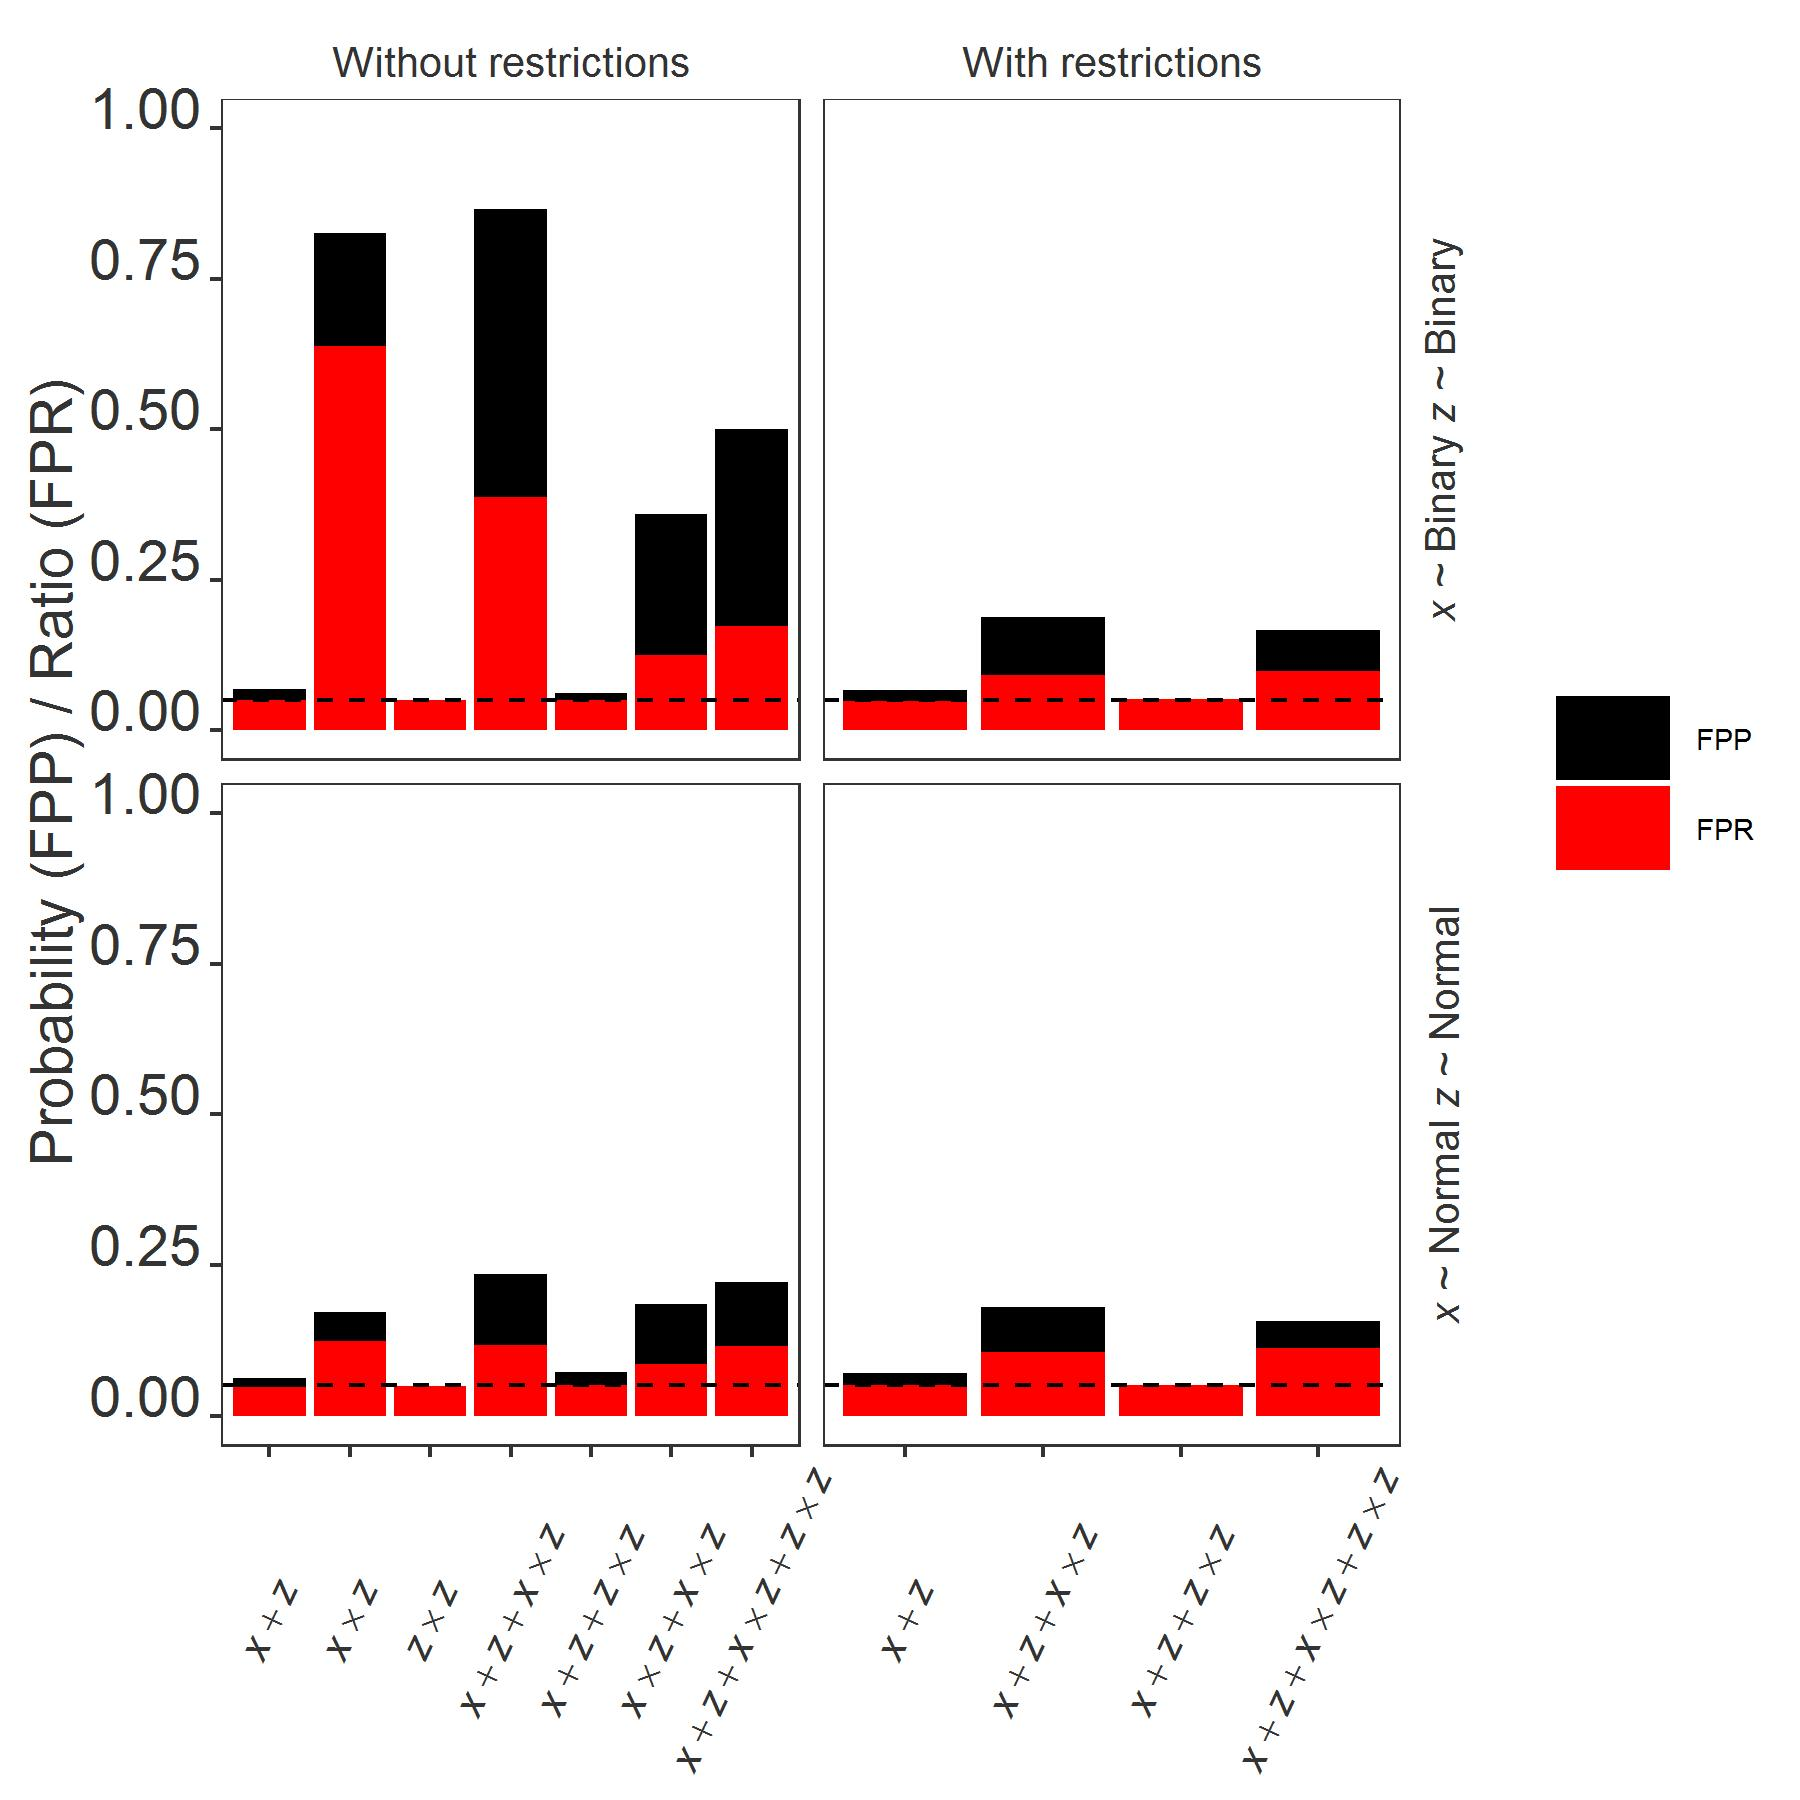
\includegraphics[width=0.7\textwidth]{R/Analysis/Result/Figures/Figure2App.jpeg}
\centering
\caption{False-positive probability and false-positive ratio when using two dependent variables and the average of the two (three dependent variables in total). The correlation between the dependent variables is set to  $\textit{r}=0.5$ with the correlation between the dependent variables and covariates still at  $\textit{r}=0.2$. Black denotes the false-positive probability and red denotes the false-positive ratio. Dashed blacked line shows the critical value, here set at 0.05. The description of the figure is otherwise the same as for Figure \ref{fig:mainfigure1}.}
\label{fig:appfigure2app}
\end{figure}

\begin{figure}[ht!]
%\figuretitle{Effect of increasing the correlation between the dependent variable and the covariates}
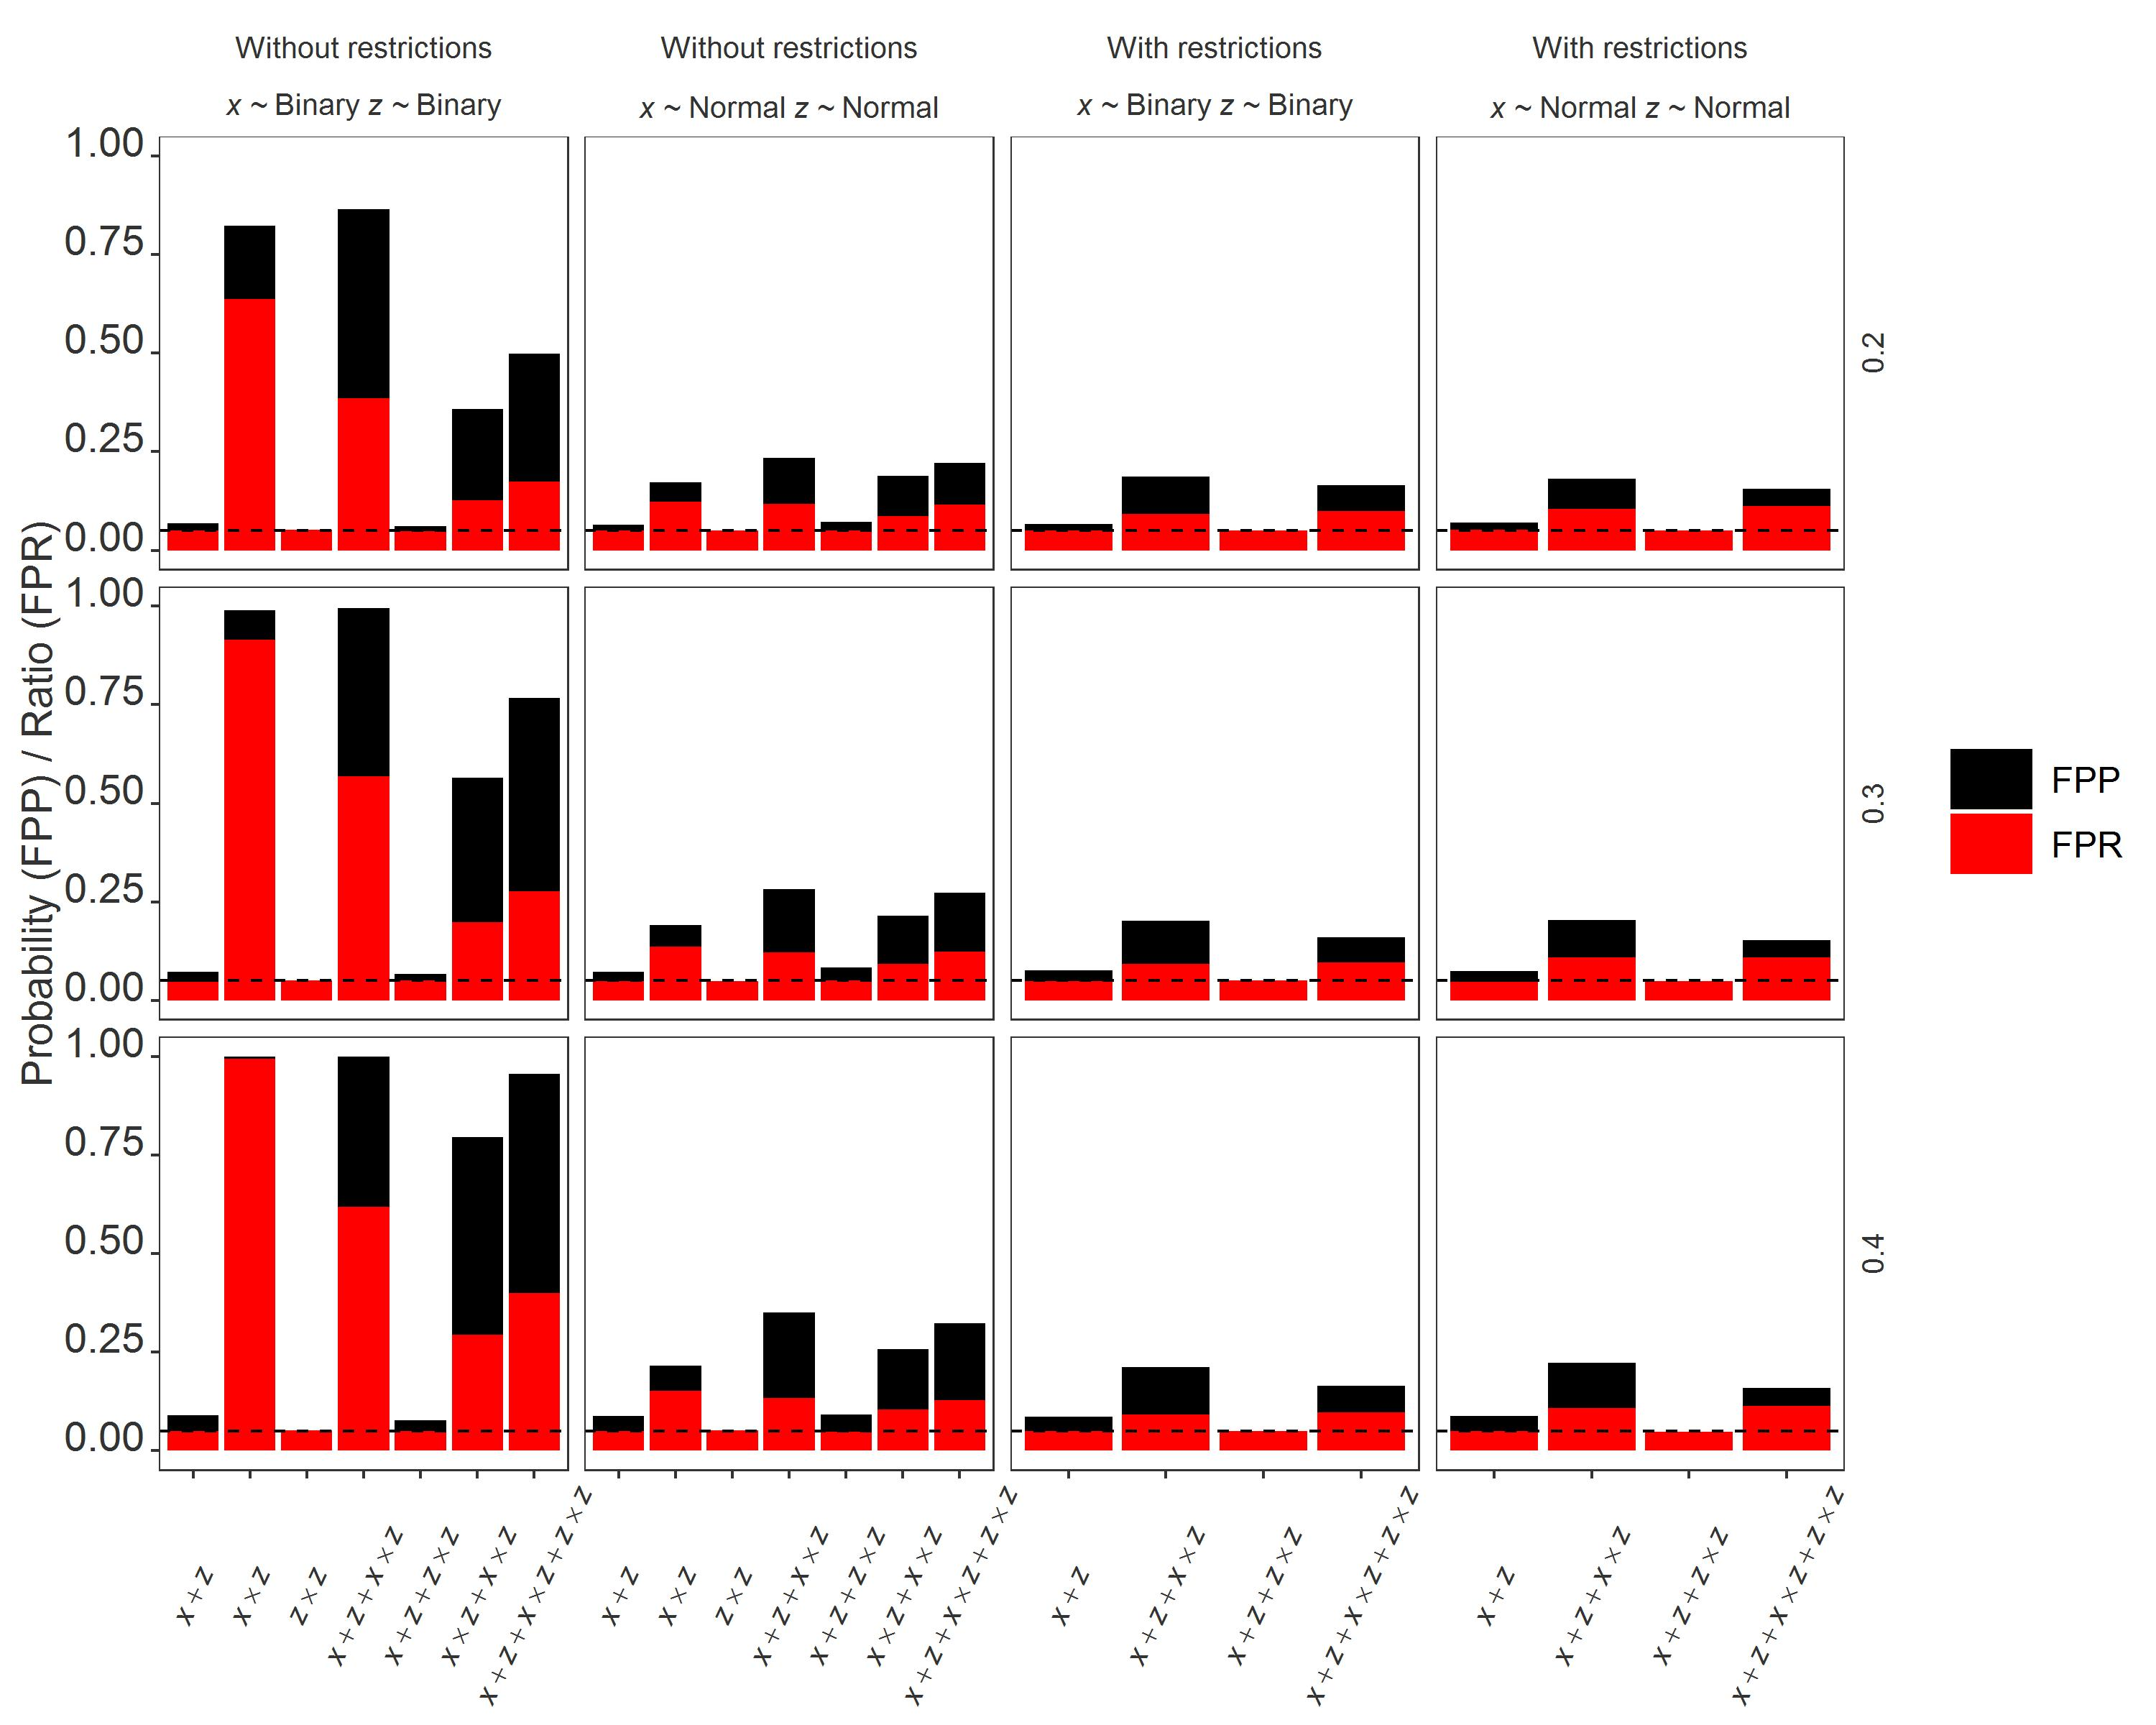
\includegraphics[width=1\textwidth]{R/Analysis/Result/Figures/Figure1App.jpeg}
\centering
\caption{False-positive probability and false-positive ratio for different levels of correlation between the dependent variable and the covariates ranging from  $\textit{r}=0.2$ to  $\textit{r}=0.4$. Black denotes the false-positive probability and red denotes the false-positive ratio. Dashed blacked line shows the critical value, here set at 0.05. The description of the figure is otherwise the same as for Figure \ref{fig:mainfigure1}.}
\label{fig:appfigure1app}
\end{figure}



\clearpage

 
% supplementary information
 
\part*{Supplementary Information} 

\begin{figure}[hbt!]
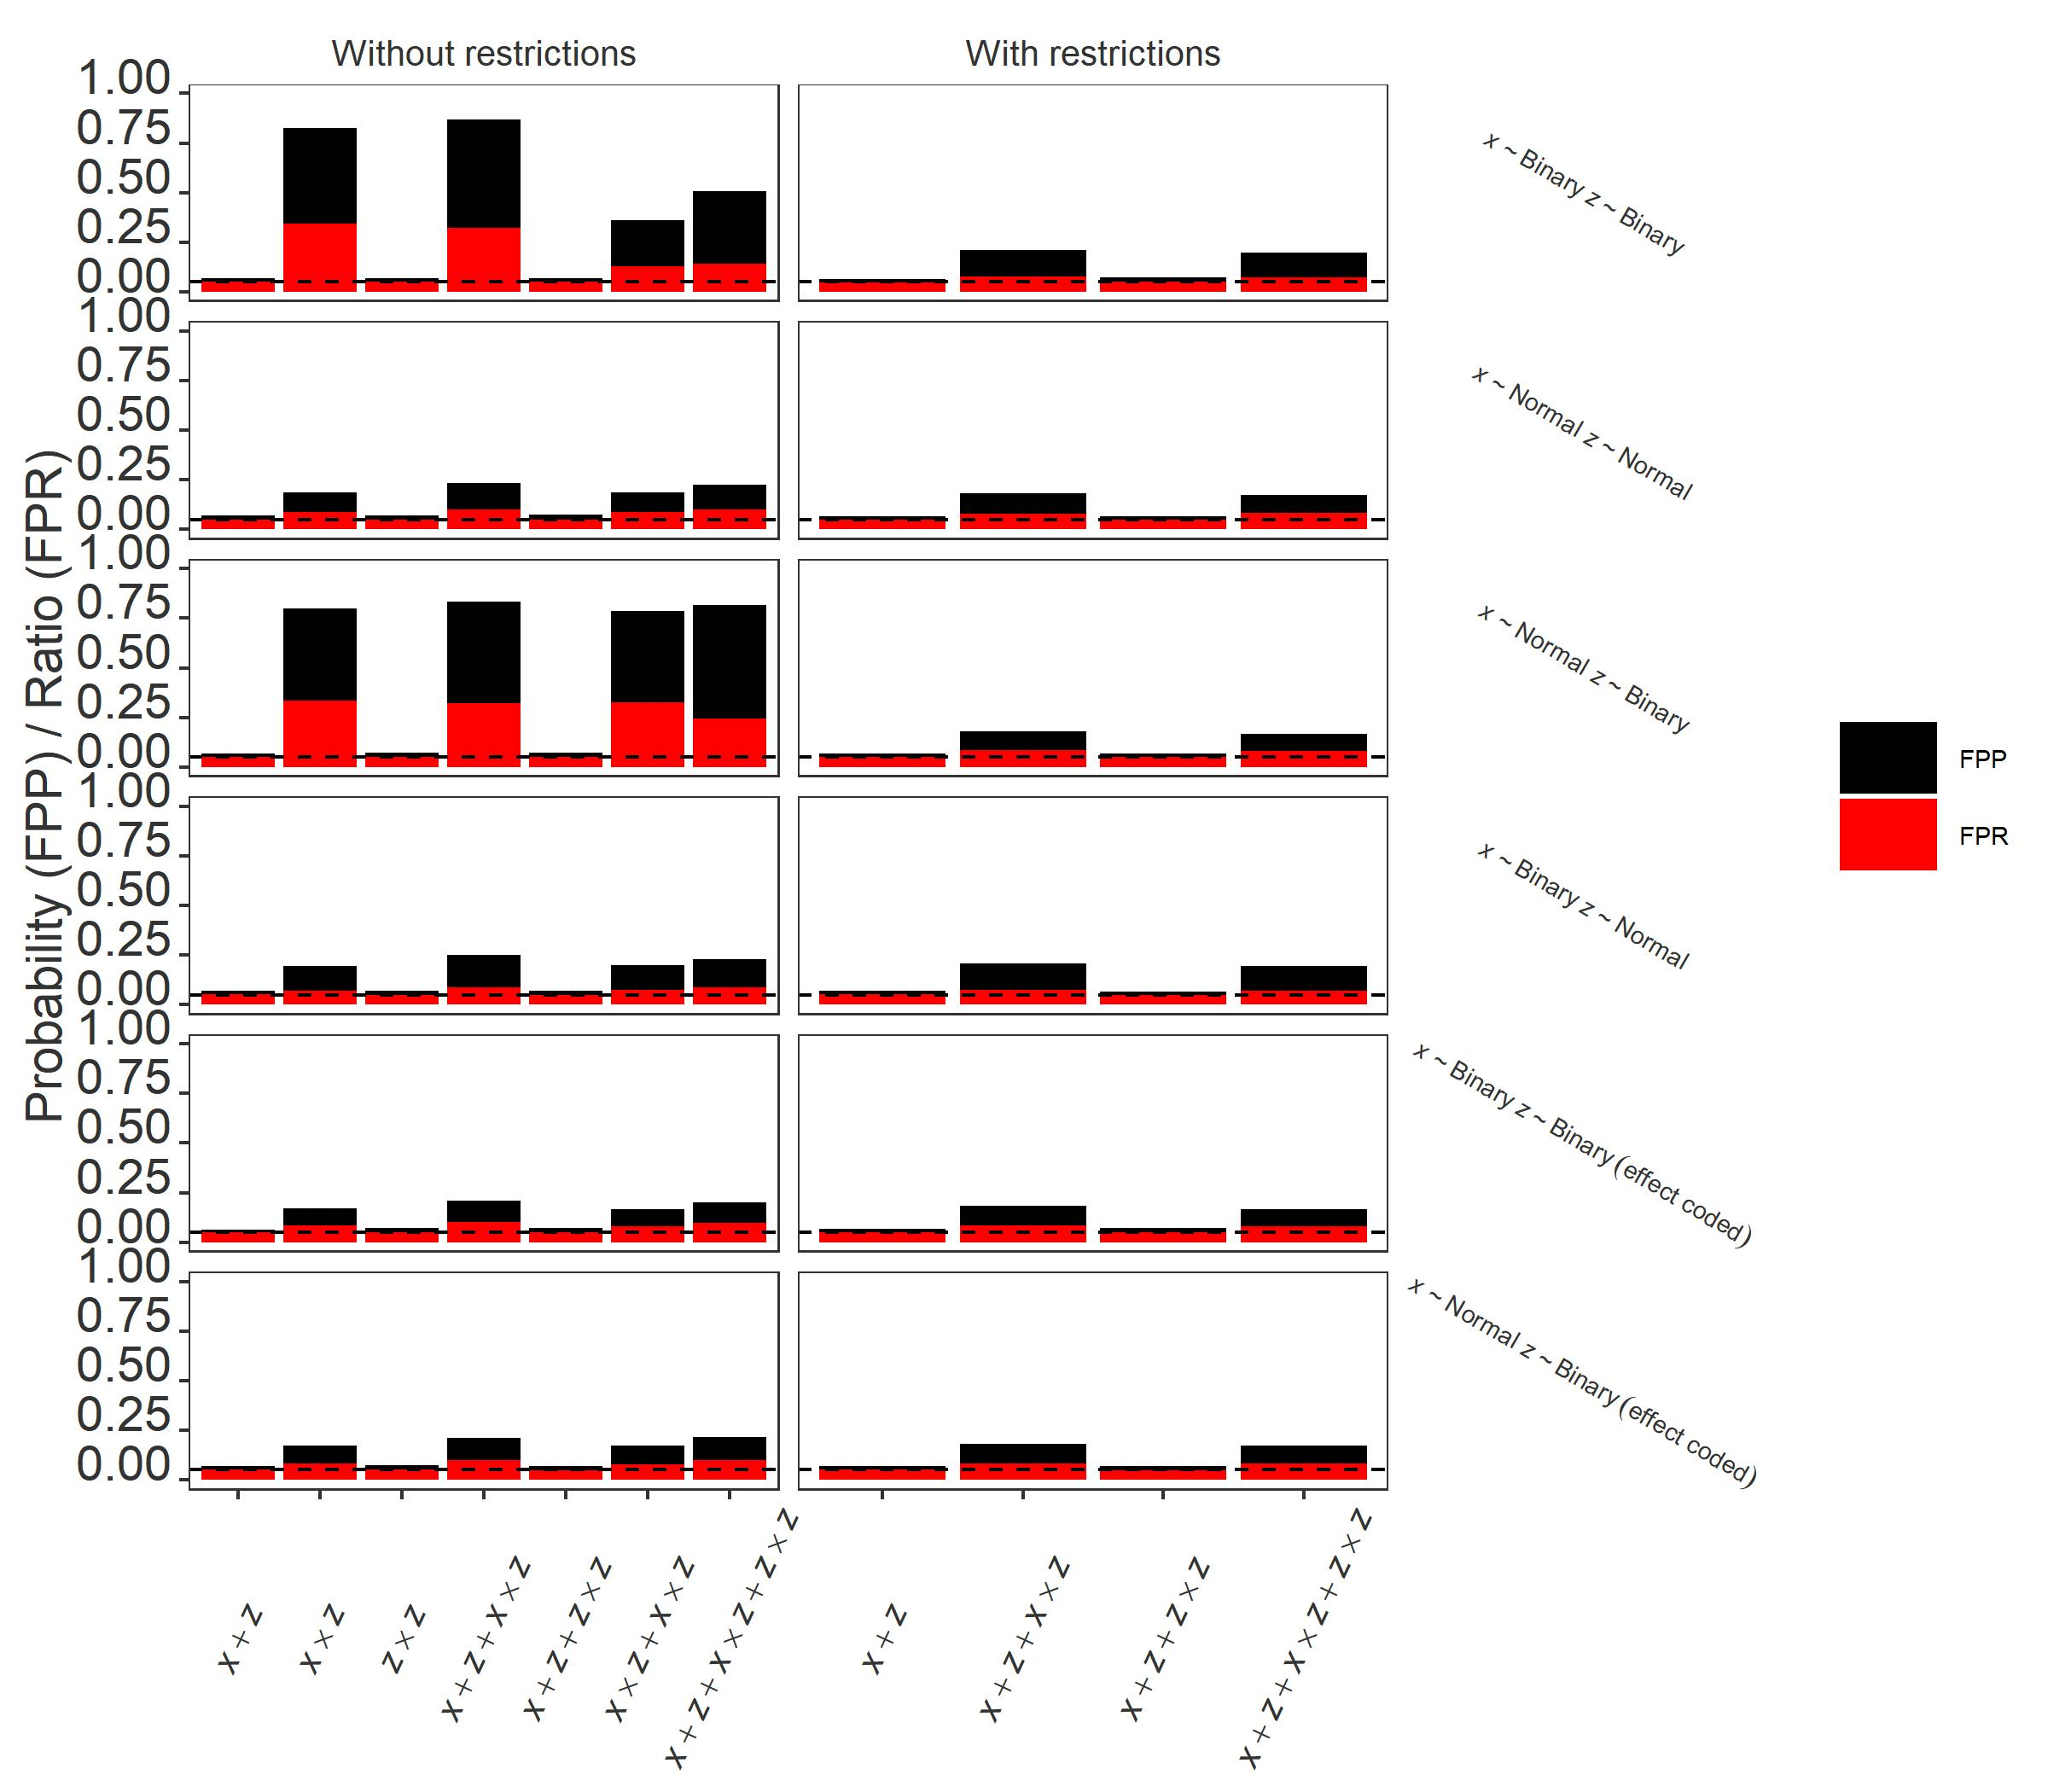
\includegraphics[scale=0.95]{R/Analysis/Result/Figures/Figure1ASI.jpeg}
\centering
\caption{The false positive probability and false positive ratio given different model sets, the presence of main effects when having interactions (i.e., With restrictions or No restrictions) and different distributions of the variable of interest and covariates. Sample size is set to 200, a correlation between the dependent variable and covariates is $\textit{r}=0.2$ and using two covariates. The false positive probability is shown in black and the false positive ratio in red. Dashed blacked line indicates 0.05. This figure adds the two other cases not shown in Figure \ref{fig:mainfigure1}}
\label{fig:appfigure1}
\end{figure}

\begin{landscape}
\begin{figure}[hbt!]
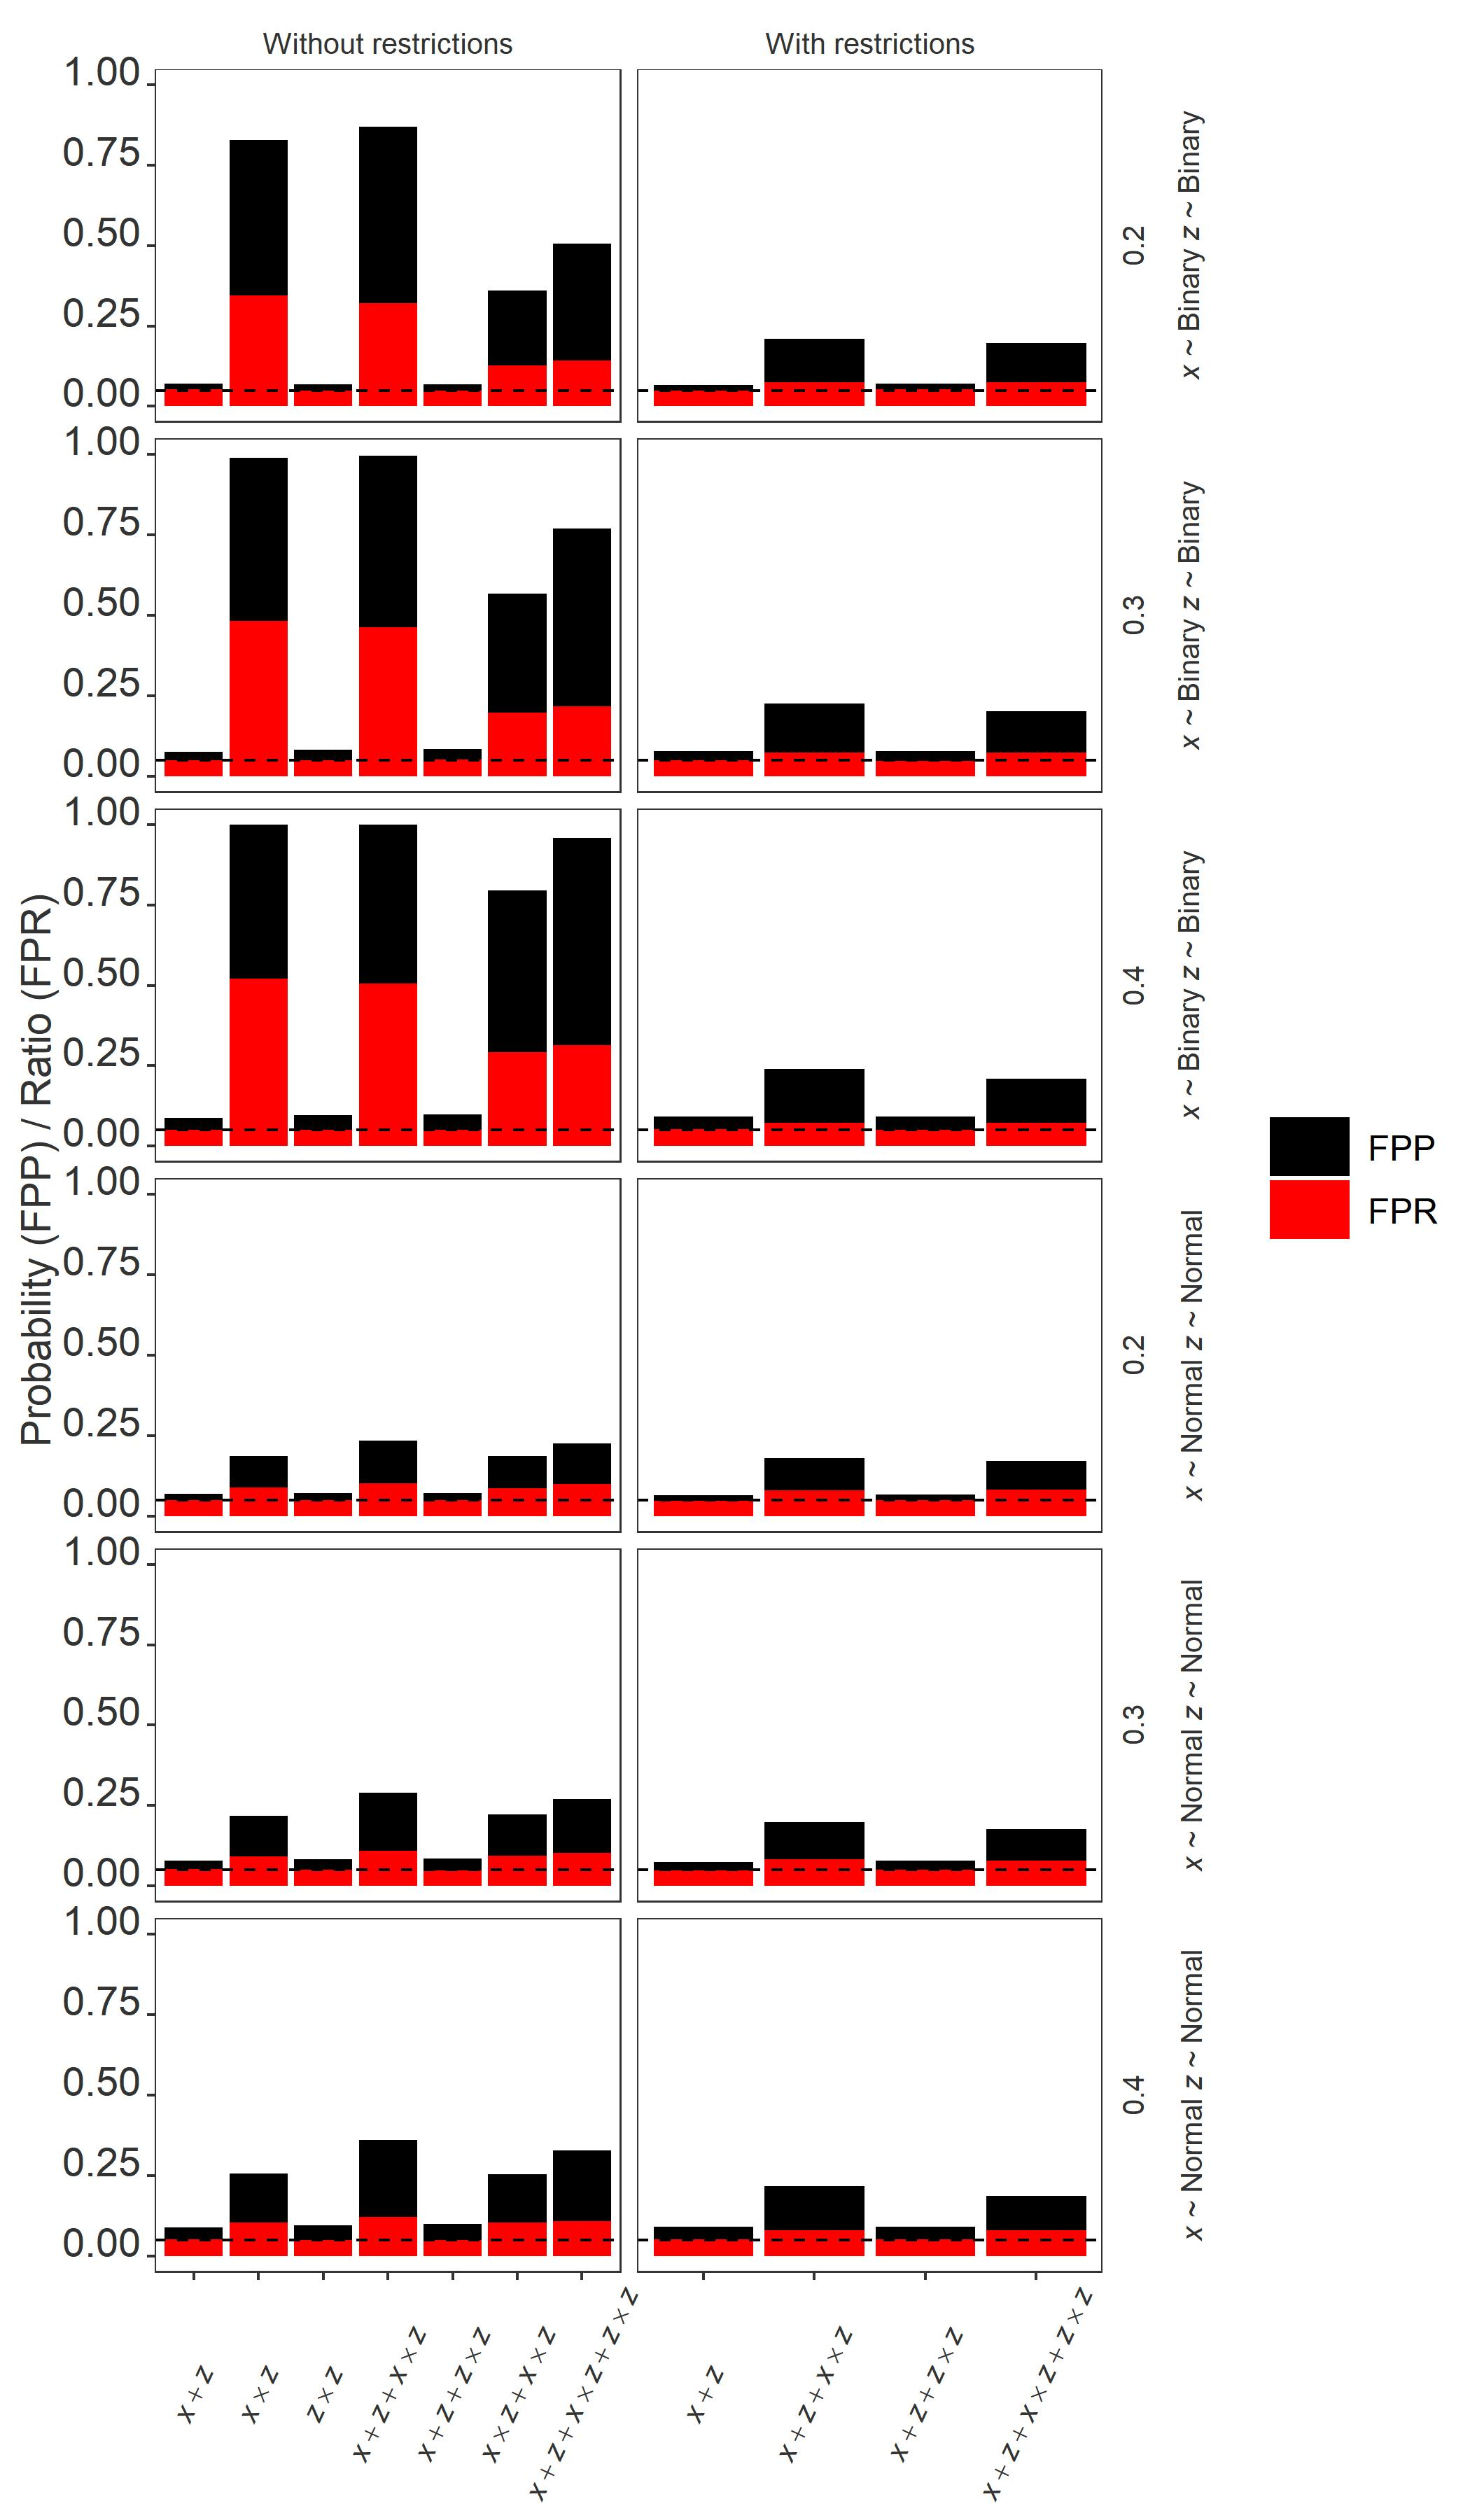
\includegraphics[scale=0.7]{R/Analysis/Result/Figures/Figure2SI.jpeg}
\centering
\caption{False positive probability and false positive for different levels of correlation between the dependent variable and the covariates ranging from  $\textit{r}=0.2$ to  $\textit{r}=0.4$. Black denotes the false positive probability and red denotes the false positive ratio. Dashed blacked line indicates 0.05. The description of the figure is otherwise the same as for Figure \ref{fig:appfigure1}.}
\label{fig:appfigure2}
\end{figure}
\end{landscape}


\begin{figure}[hbt!]
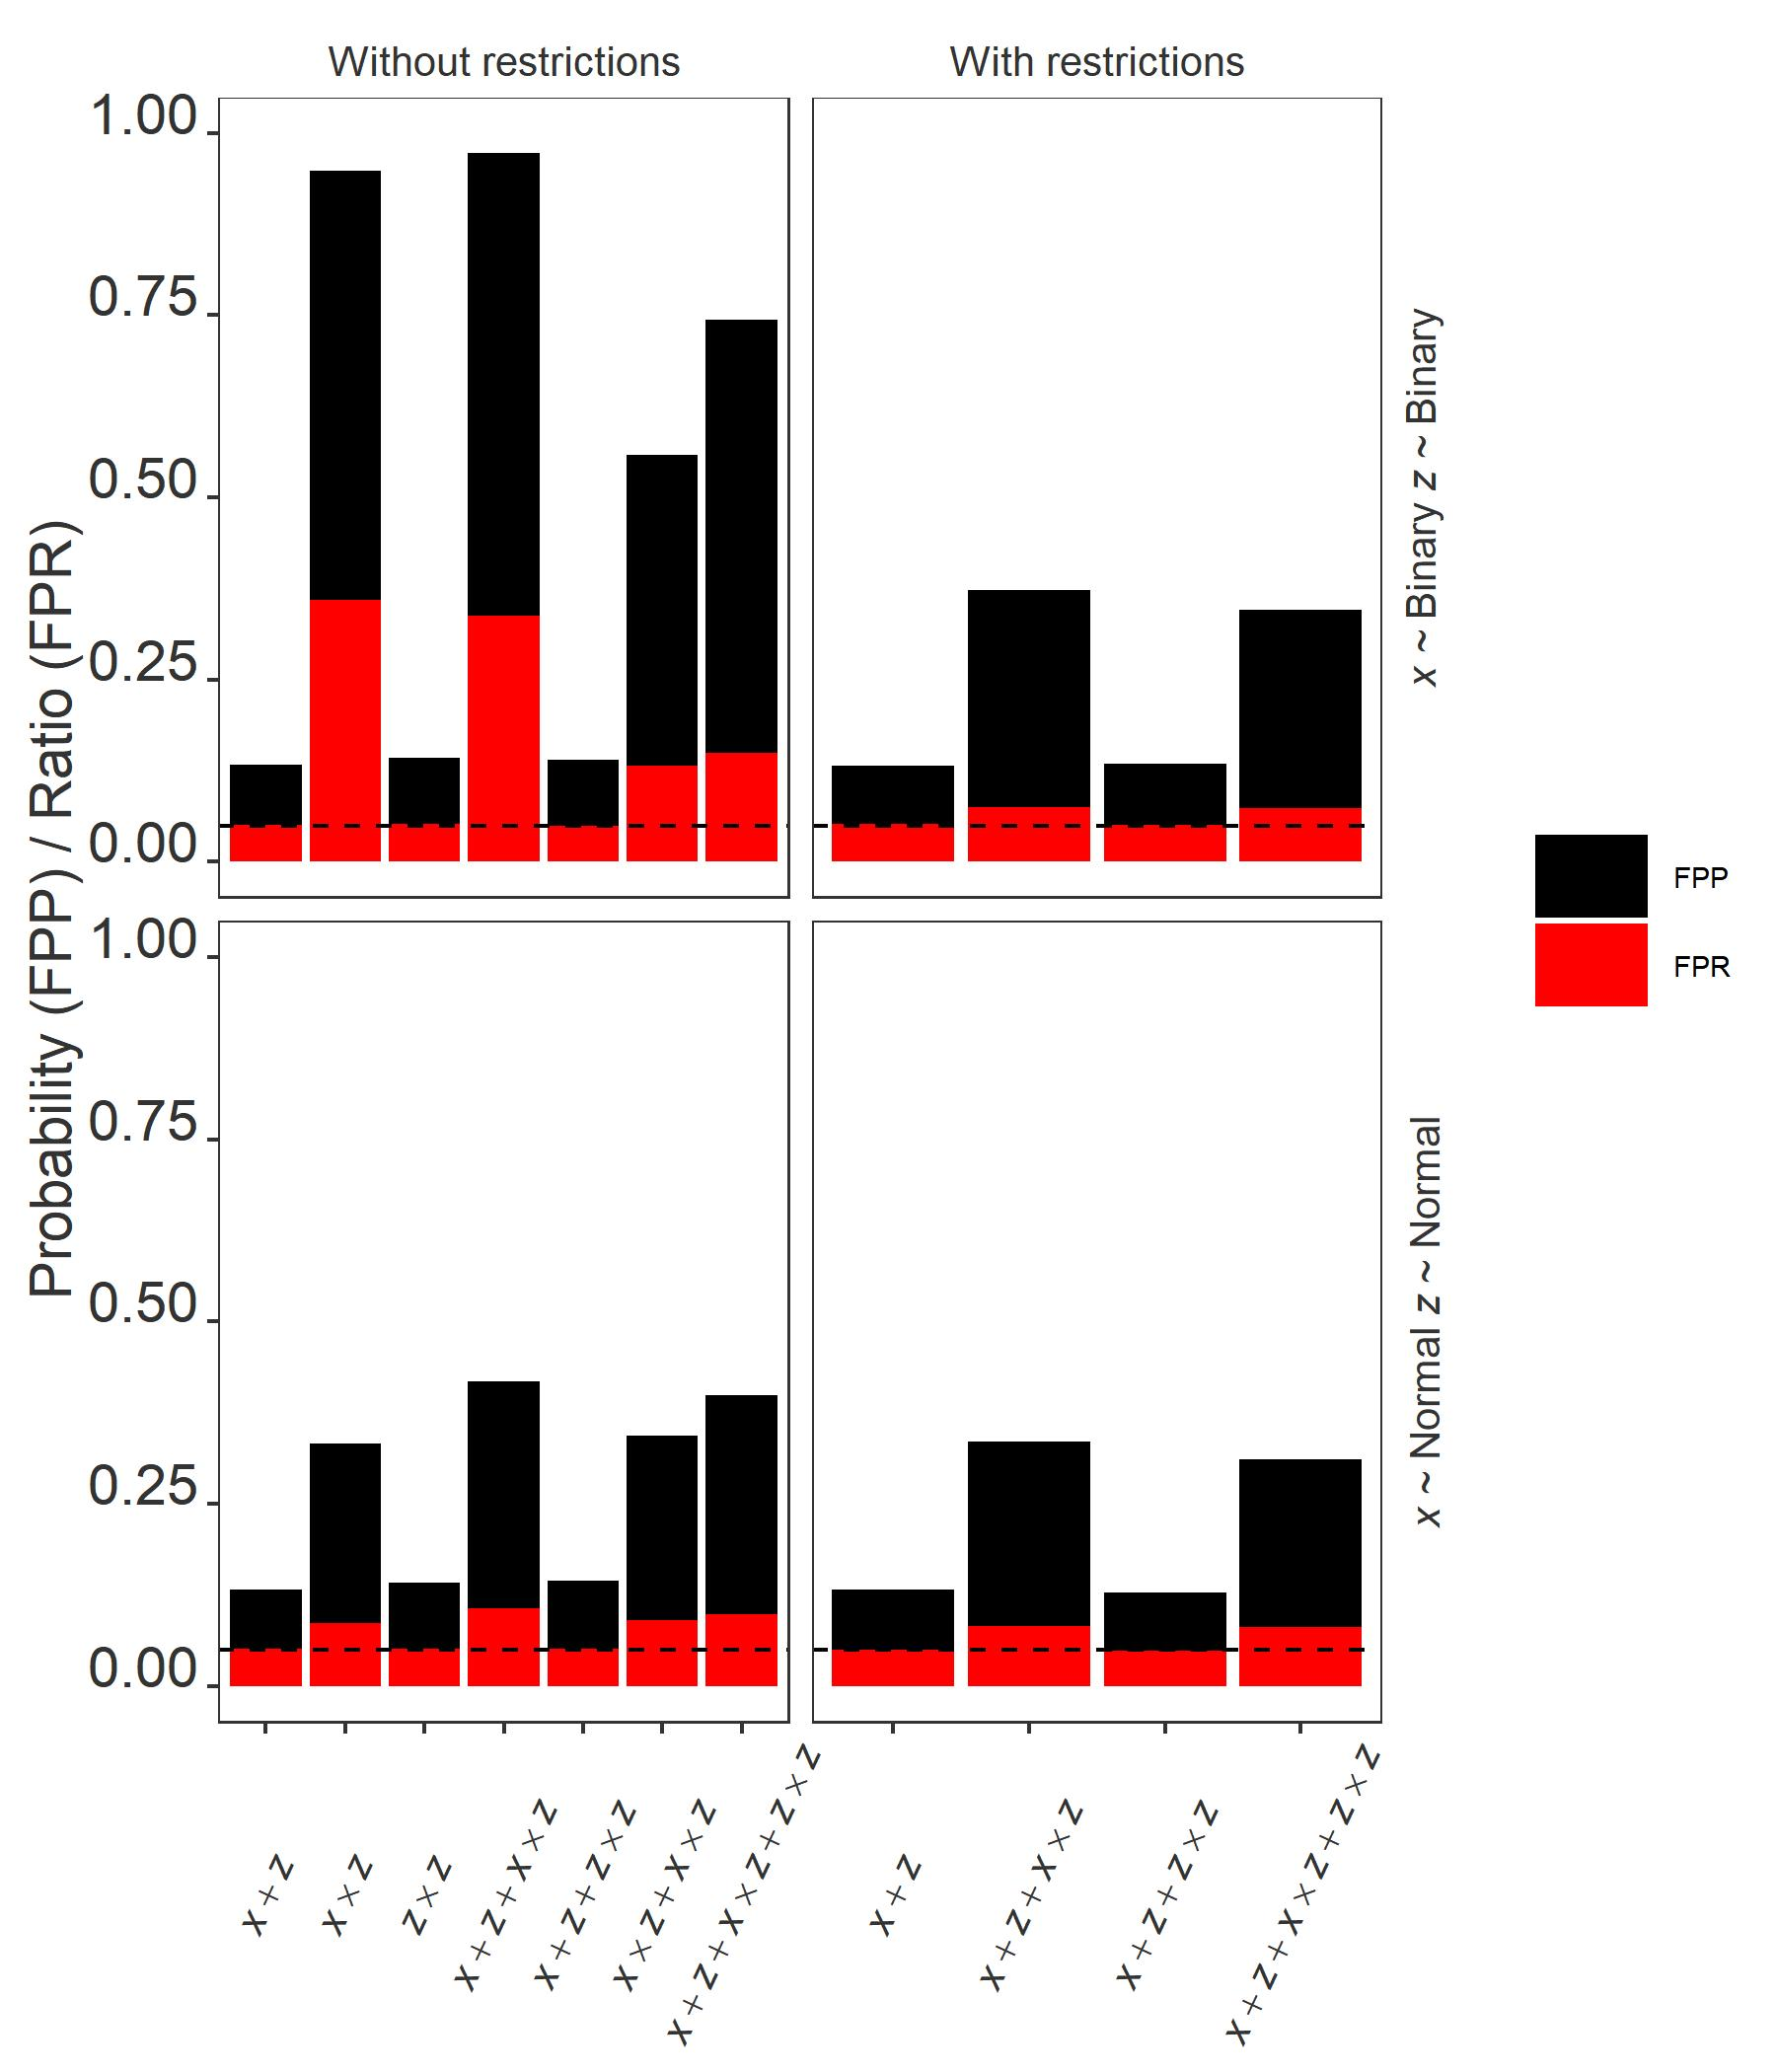
\includegraphics{R/Analysis/Result/Figures/Figure3SI.jpeg}
\centering
\caption{False positive probability and false positive ratio when using two dependent variables and the average of the two (meaning three dependent variables in total). The correlation between the dependent variables is set to  $\textit{r}=0.5$ with the correlation between the dependent variables and covariates still at  $\textit{r}=0.2$. Black denotes the the false positive probability and red denotes the false positive ratio. Dashed blacked line indicates 0.05. The description of the figure is otherwise the same as for Figure \ref{fig:appfigure1}.}
\label{fig:appfigure3}
\end{figure}


\begin{figure}[hbt!]
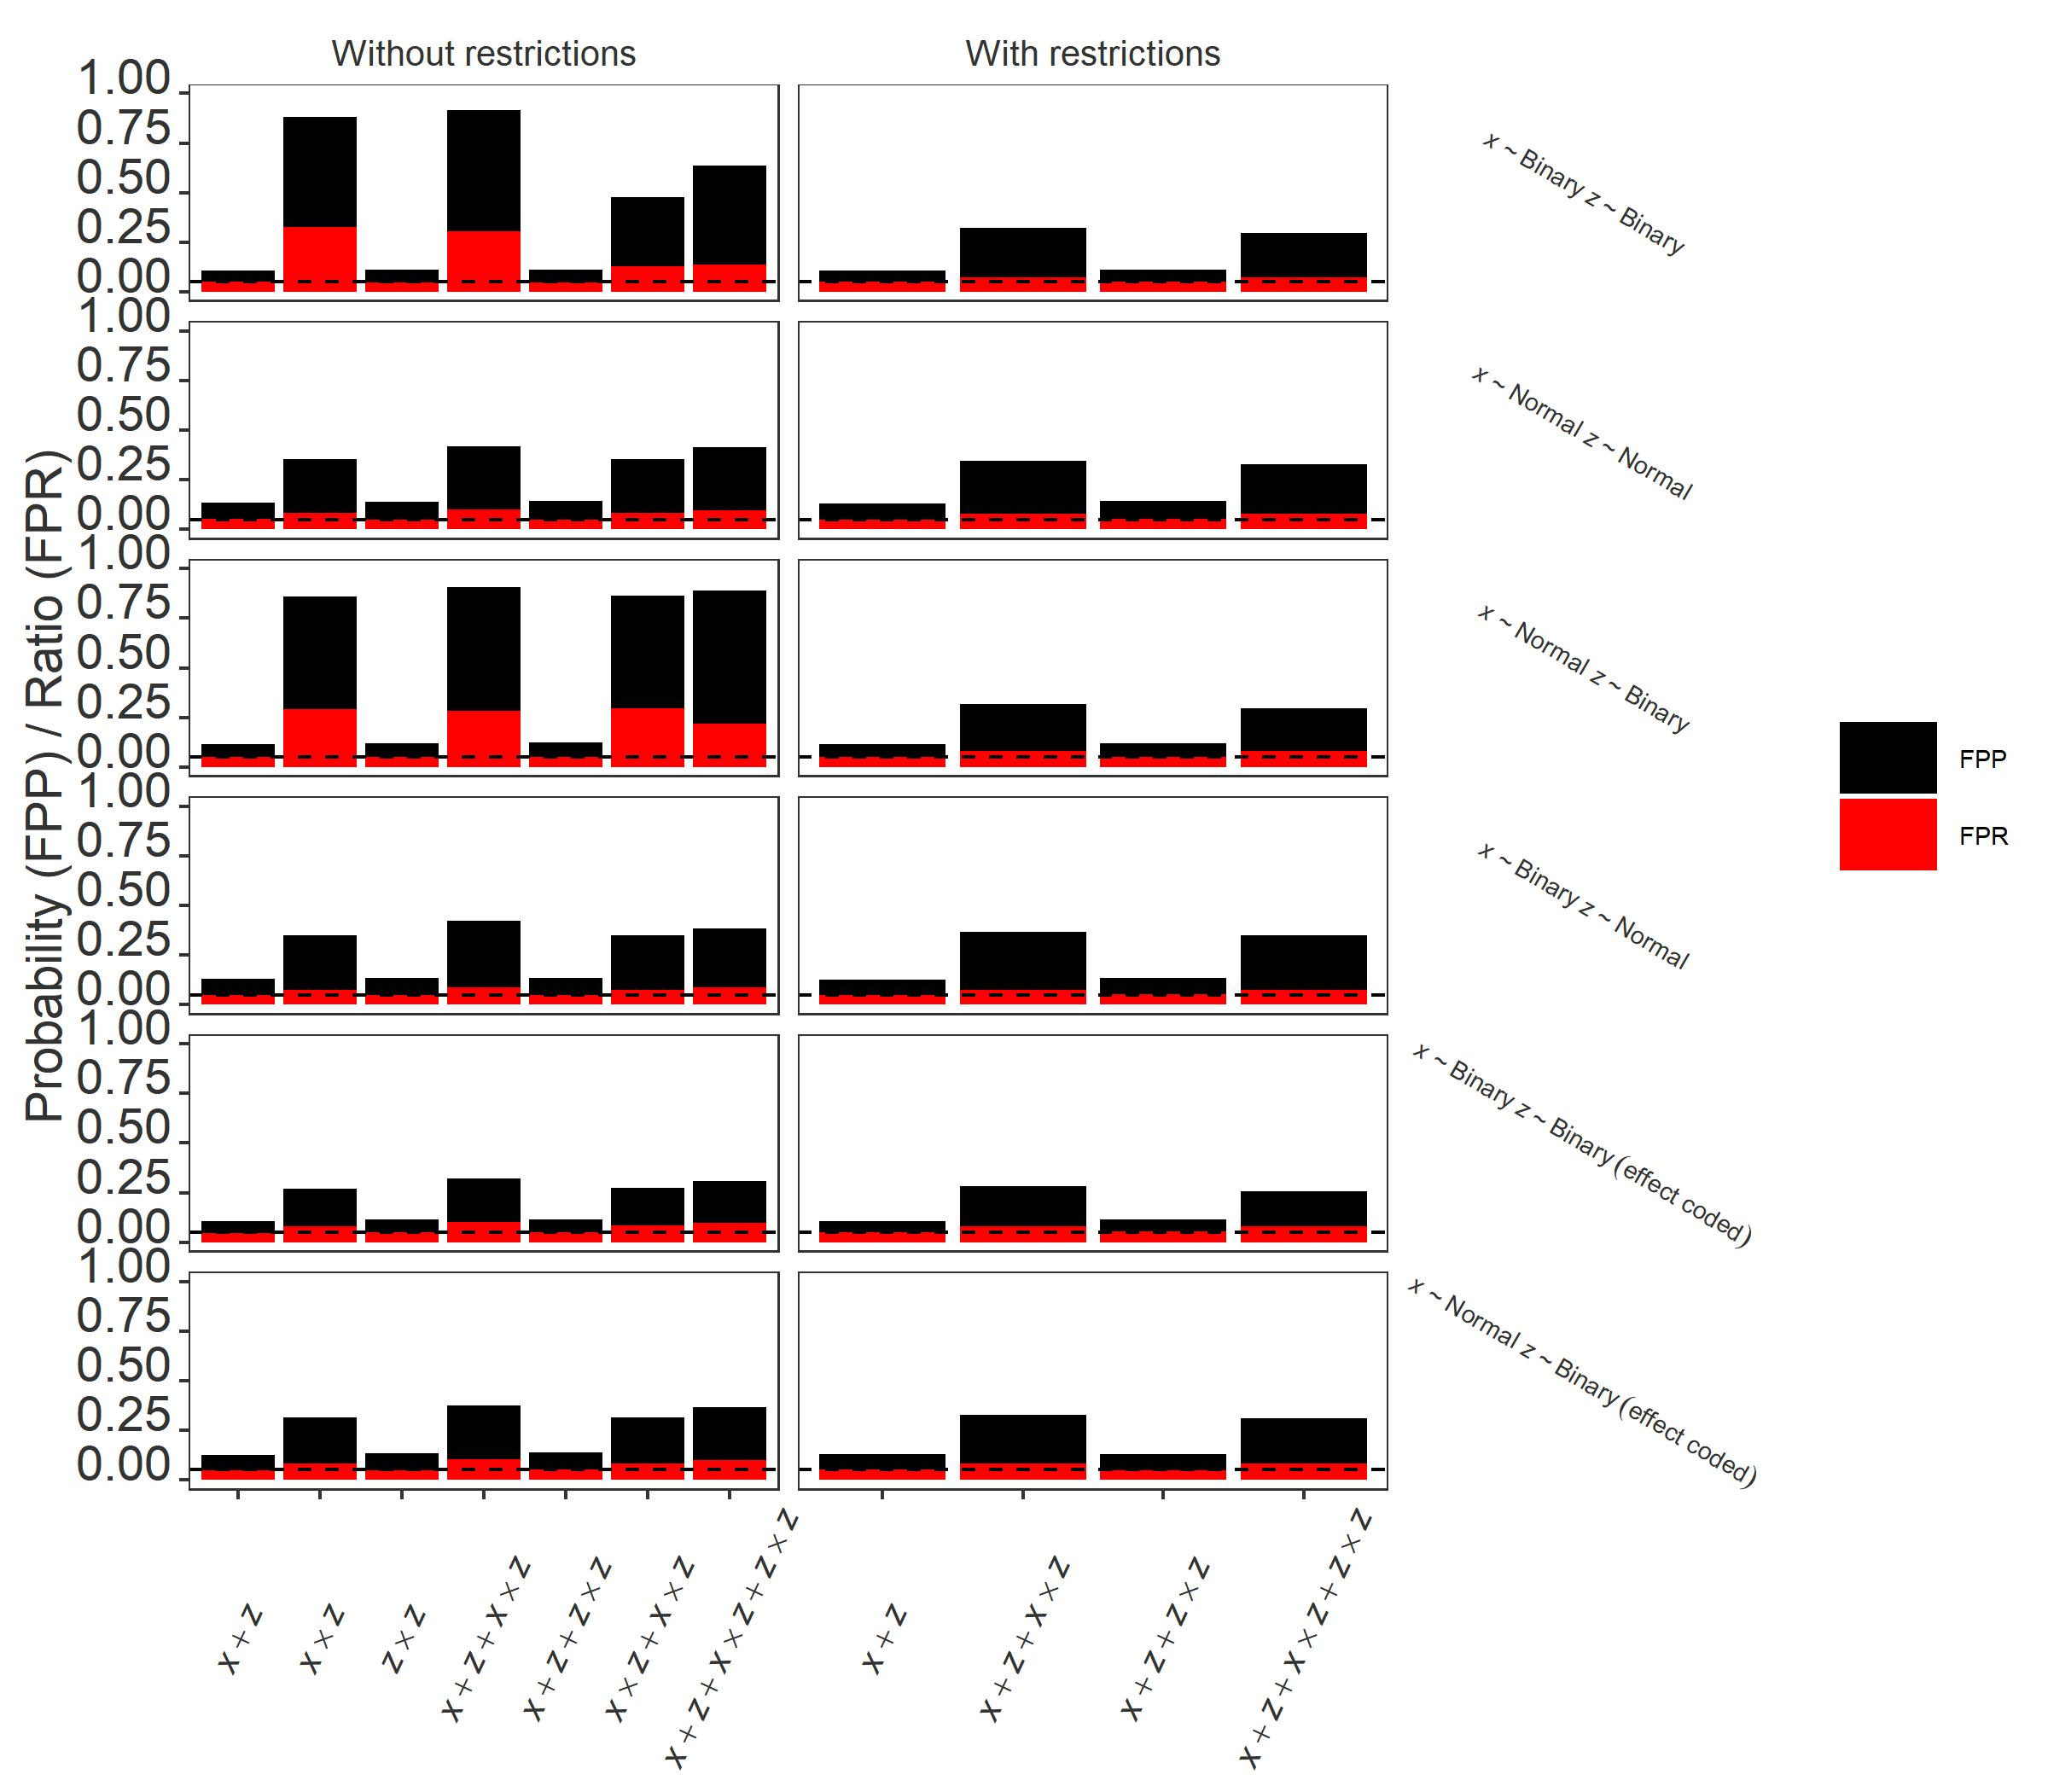
\includegraphics[scale=0.95]{R/Analysis/Result/Figures/Figure1BSI.jpeg}
\centering
\caption{False positive probability and false positive ratio when using multiple outlier criteria. Black denotes the the false positive probability and red denotes the false positive ratio. Dashed blacked line indicates 0.05. The description of the figure is otherwise the same as for Figure \ref{fig:appfigure1}. This figure adds the two other cases not shown in Figure \ref{fig:mainfigure3}.
}
\label{fig:appfigure4}
\end{figure}

\begin{figure}[hbt!]
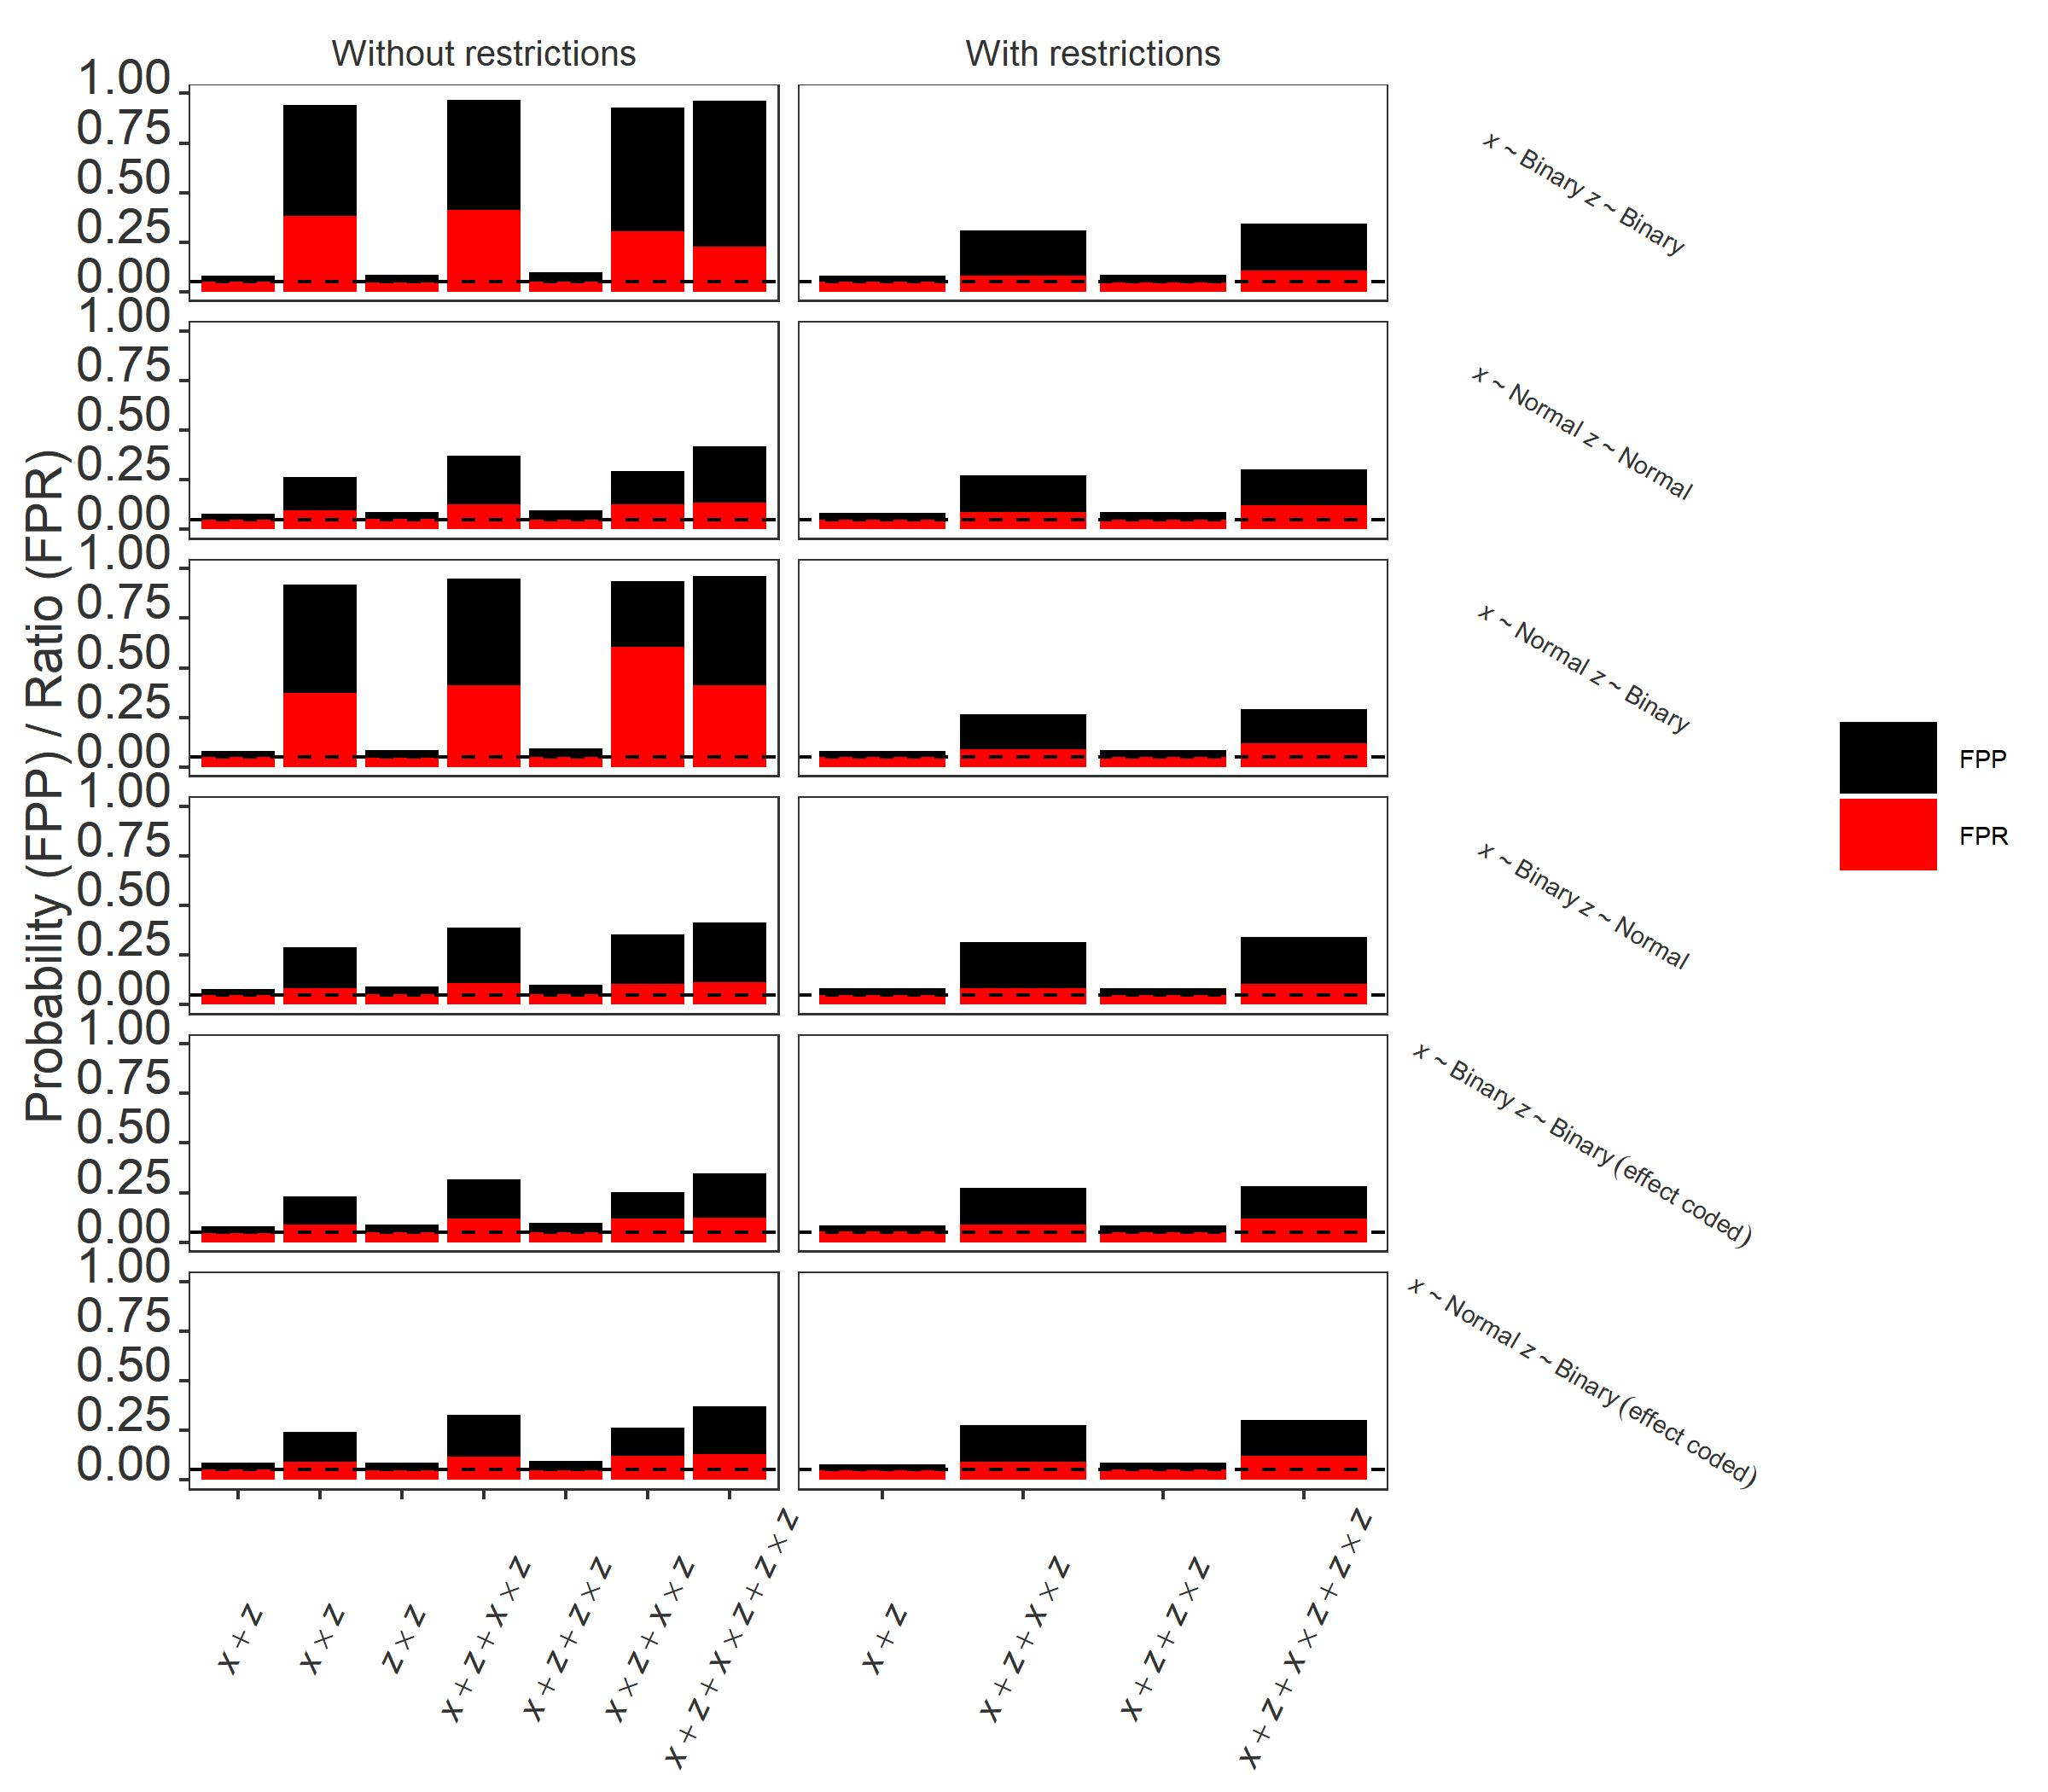
\includegraphics[scale=0.95]{R/Analysis/Result/Figures/Figure1CSI.jpeg}
\centering
\caption{False positive probability and false positive ratio when using three covariates instead of two as in the base line model. Black denotes the the false positive probability and red denotes the false positive ratio. Dashed blacked line indicates 0.05. The description of the figure is otherwise the same as for Figure \ref{fig:appfigure1}. This figure adds the two other cases not shown in Figure \ref{fig:mainfigure2}.
}
\label{fig:appfigure5}
\end{figure}

\begin{landscape}
\begin{figure}[hbt!]
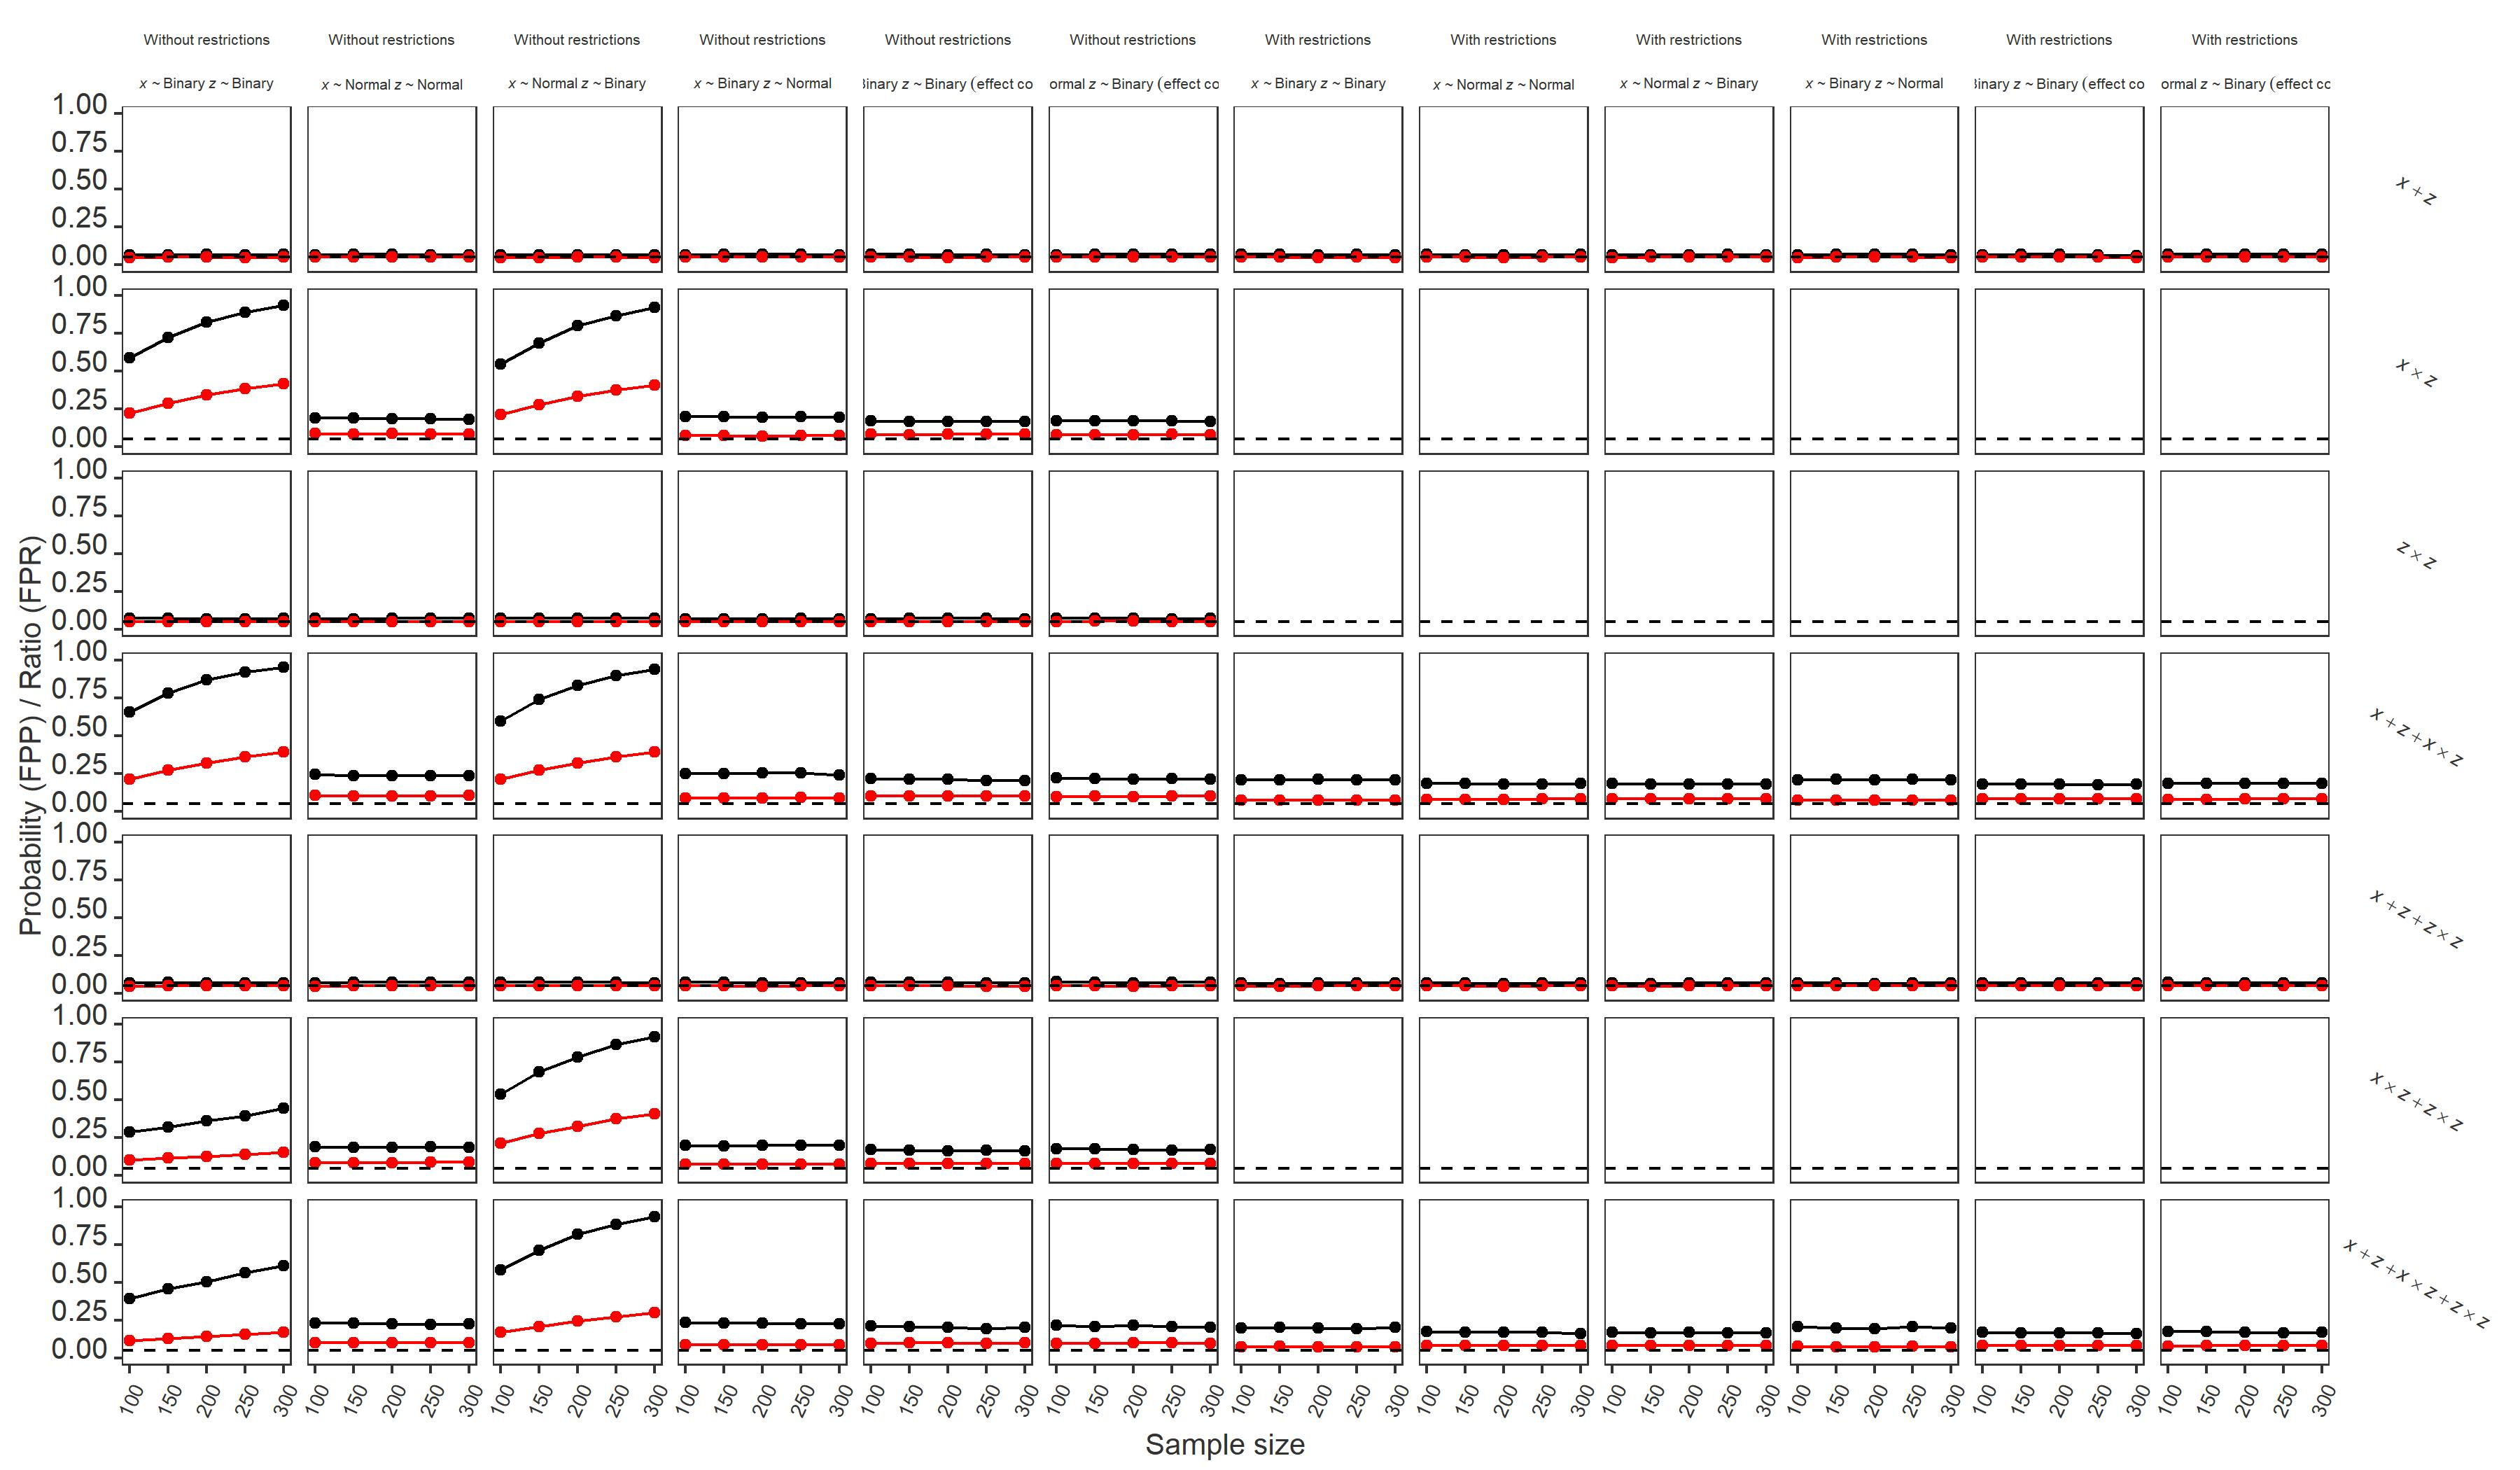
\includegraphics[scale=0.75]{R/Analysis/Result/Figures/Figure1DSI.jpeg}
\centering
\caption{Effect of increasing sample size for each model set and all combinations of data distributions (i.e., binary and normal). Black denotes the false positive probability and red denotes the false positive ratio. Dashed blacked line indicates 0.05. The description of the figure is otherwise the same as for Figure \ref{fig:appfigure1}. This figure adds the two other cases not shown in Figure \ref{fig:mainfigure4}}
\label{fig:appfigure6}
\end{figure}
\end{landscape}

\clearpage
\subsection{Results when using Bonferroni correction}

In this section, we present the same analyses but with Bonferroni correction applied. This means that the critical value ($\alpha$) now has a correction such that $\alpha = 0.05 / #Number~of~test~in~each~set$. So the critical value will only be 0.05 in the case where there is no interactions between the variable of interest and the covariates. The critical value is corrected for each test such that it can differ within each model set depending on how many interactions there are per model. 

Table \ref{tab:resultFullBC} shows the FPP and FPR for the full model sets under different conditions when there is used Bonferroni correction. Here there is no split between each model set.This lowers the FPR to the expected 5\% but there is still an issue when not including main effects and having binomial variables. 

% latex table generated in R 4.0.0 by xtable 1.8-4 package
% Wed Feb 03 15:03:29 2021
\begin{longtable}{llrr}
\caption{False positive probability (FPP) and false positive ratio (FPR) when looking at all the models possible when the sample size is 200, no outlier criteria is being used and having two covariates. When restrictions on interactions are on main effects should always be present when there is interactions, this is not the case when restrictions on interactions is off.} \\ 
  \hline
Restrictions on interactions & Type & FPP & FPR \\ 
  \hline
Without & Normal & 0.25 & 0.10 \\ 
  Without & Binomial & 0.87 & 0.23 \\ 
  With & Normal & 0.19 & 0.08 \\ 
  With & Binomial & 0.21 & 0.08 \\ 
   \hline
\hline
\end{longtable}


\begin{figure}[hbt!]
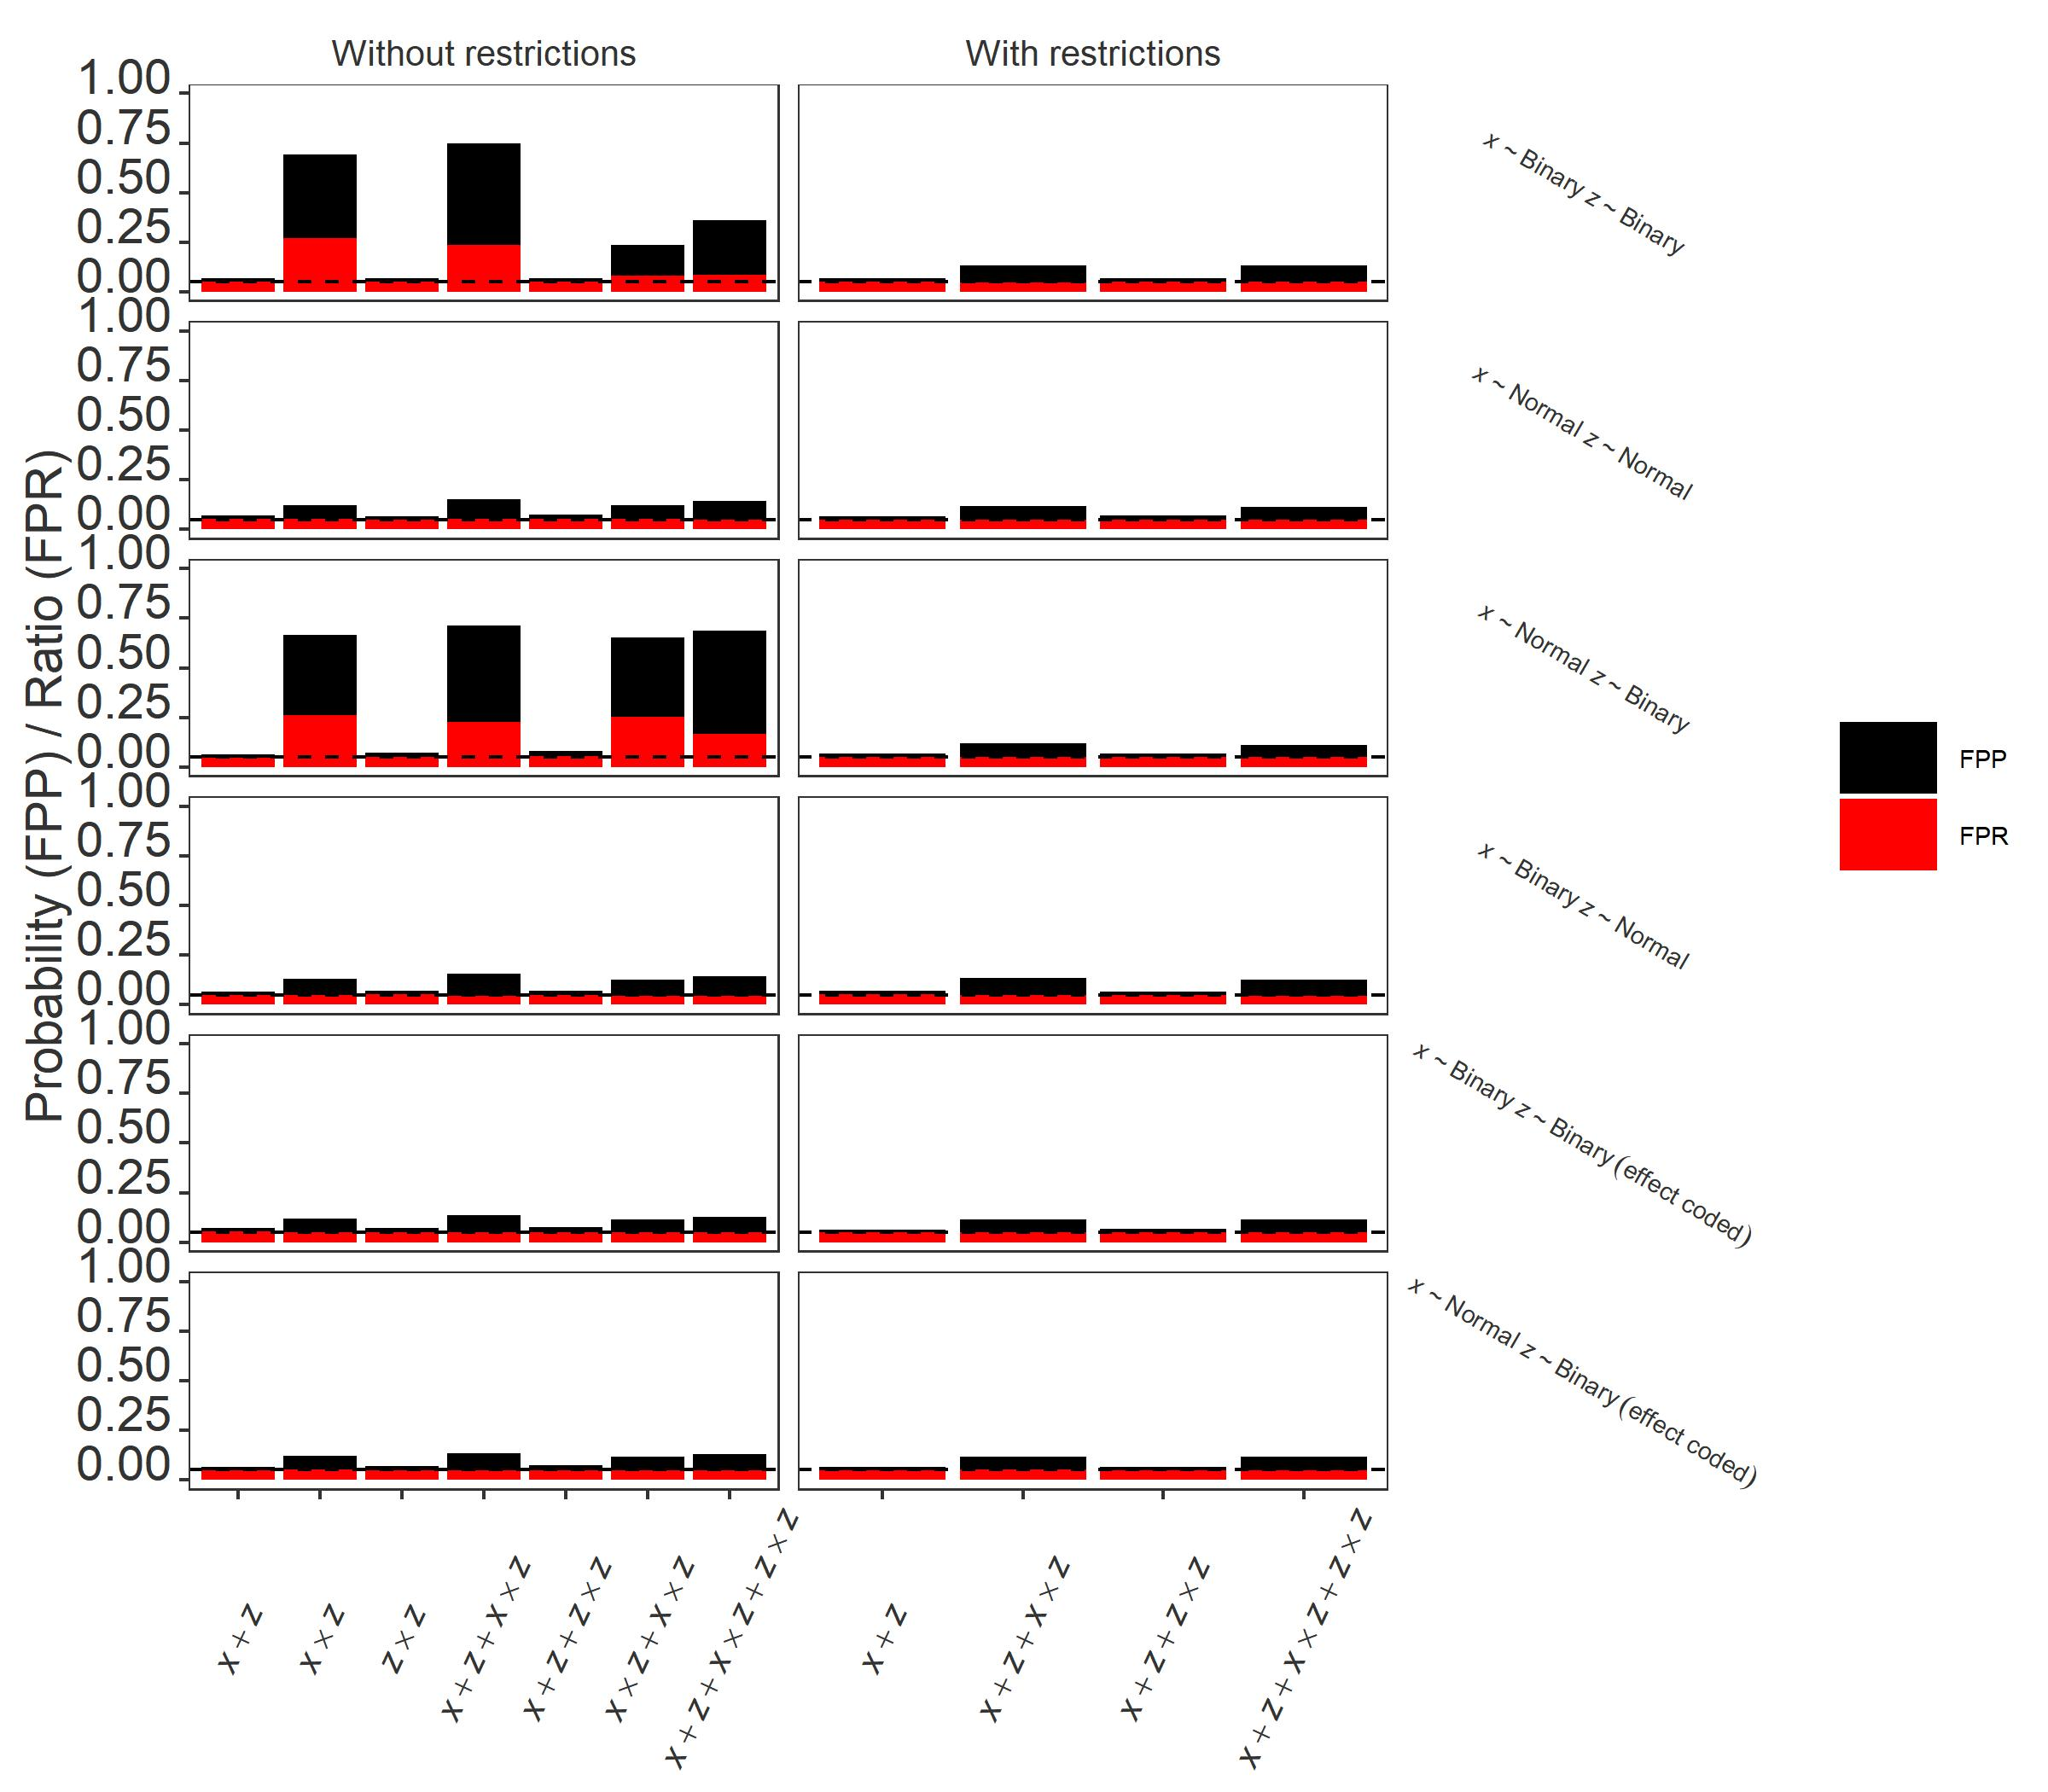
\includegraphics[scale=0.95]{R/Analysis/Result/Figures/Figure1ASIBon.jpeg}
\centering
\caption{The description of this figure is the same as for Figure \ref{fig:appfigure1} with the only difference being that we applied Bonferroni correction. This figure therefore shows the probability of the false positive probability and false positive ratio given different model sets, the presence of main effects when having interactions (i.e., With restrictions for interactions or No restrictions for interactions) and different distributions of the variable of interest and covariates. Sample size was set to 200, a correlation between the dependent variable and covariates was $\textit{r}=0.2$ and we used two covariates. The false positive probability is shown in black and the false positive ratio in red. Dashed blacked line indicates 0.05. }
\label{fig:appfigure7}
\end{figure}

\begin{landscape}
\begin{figure}[hbt!]
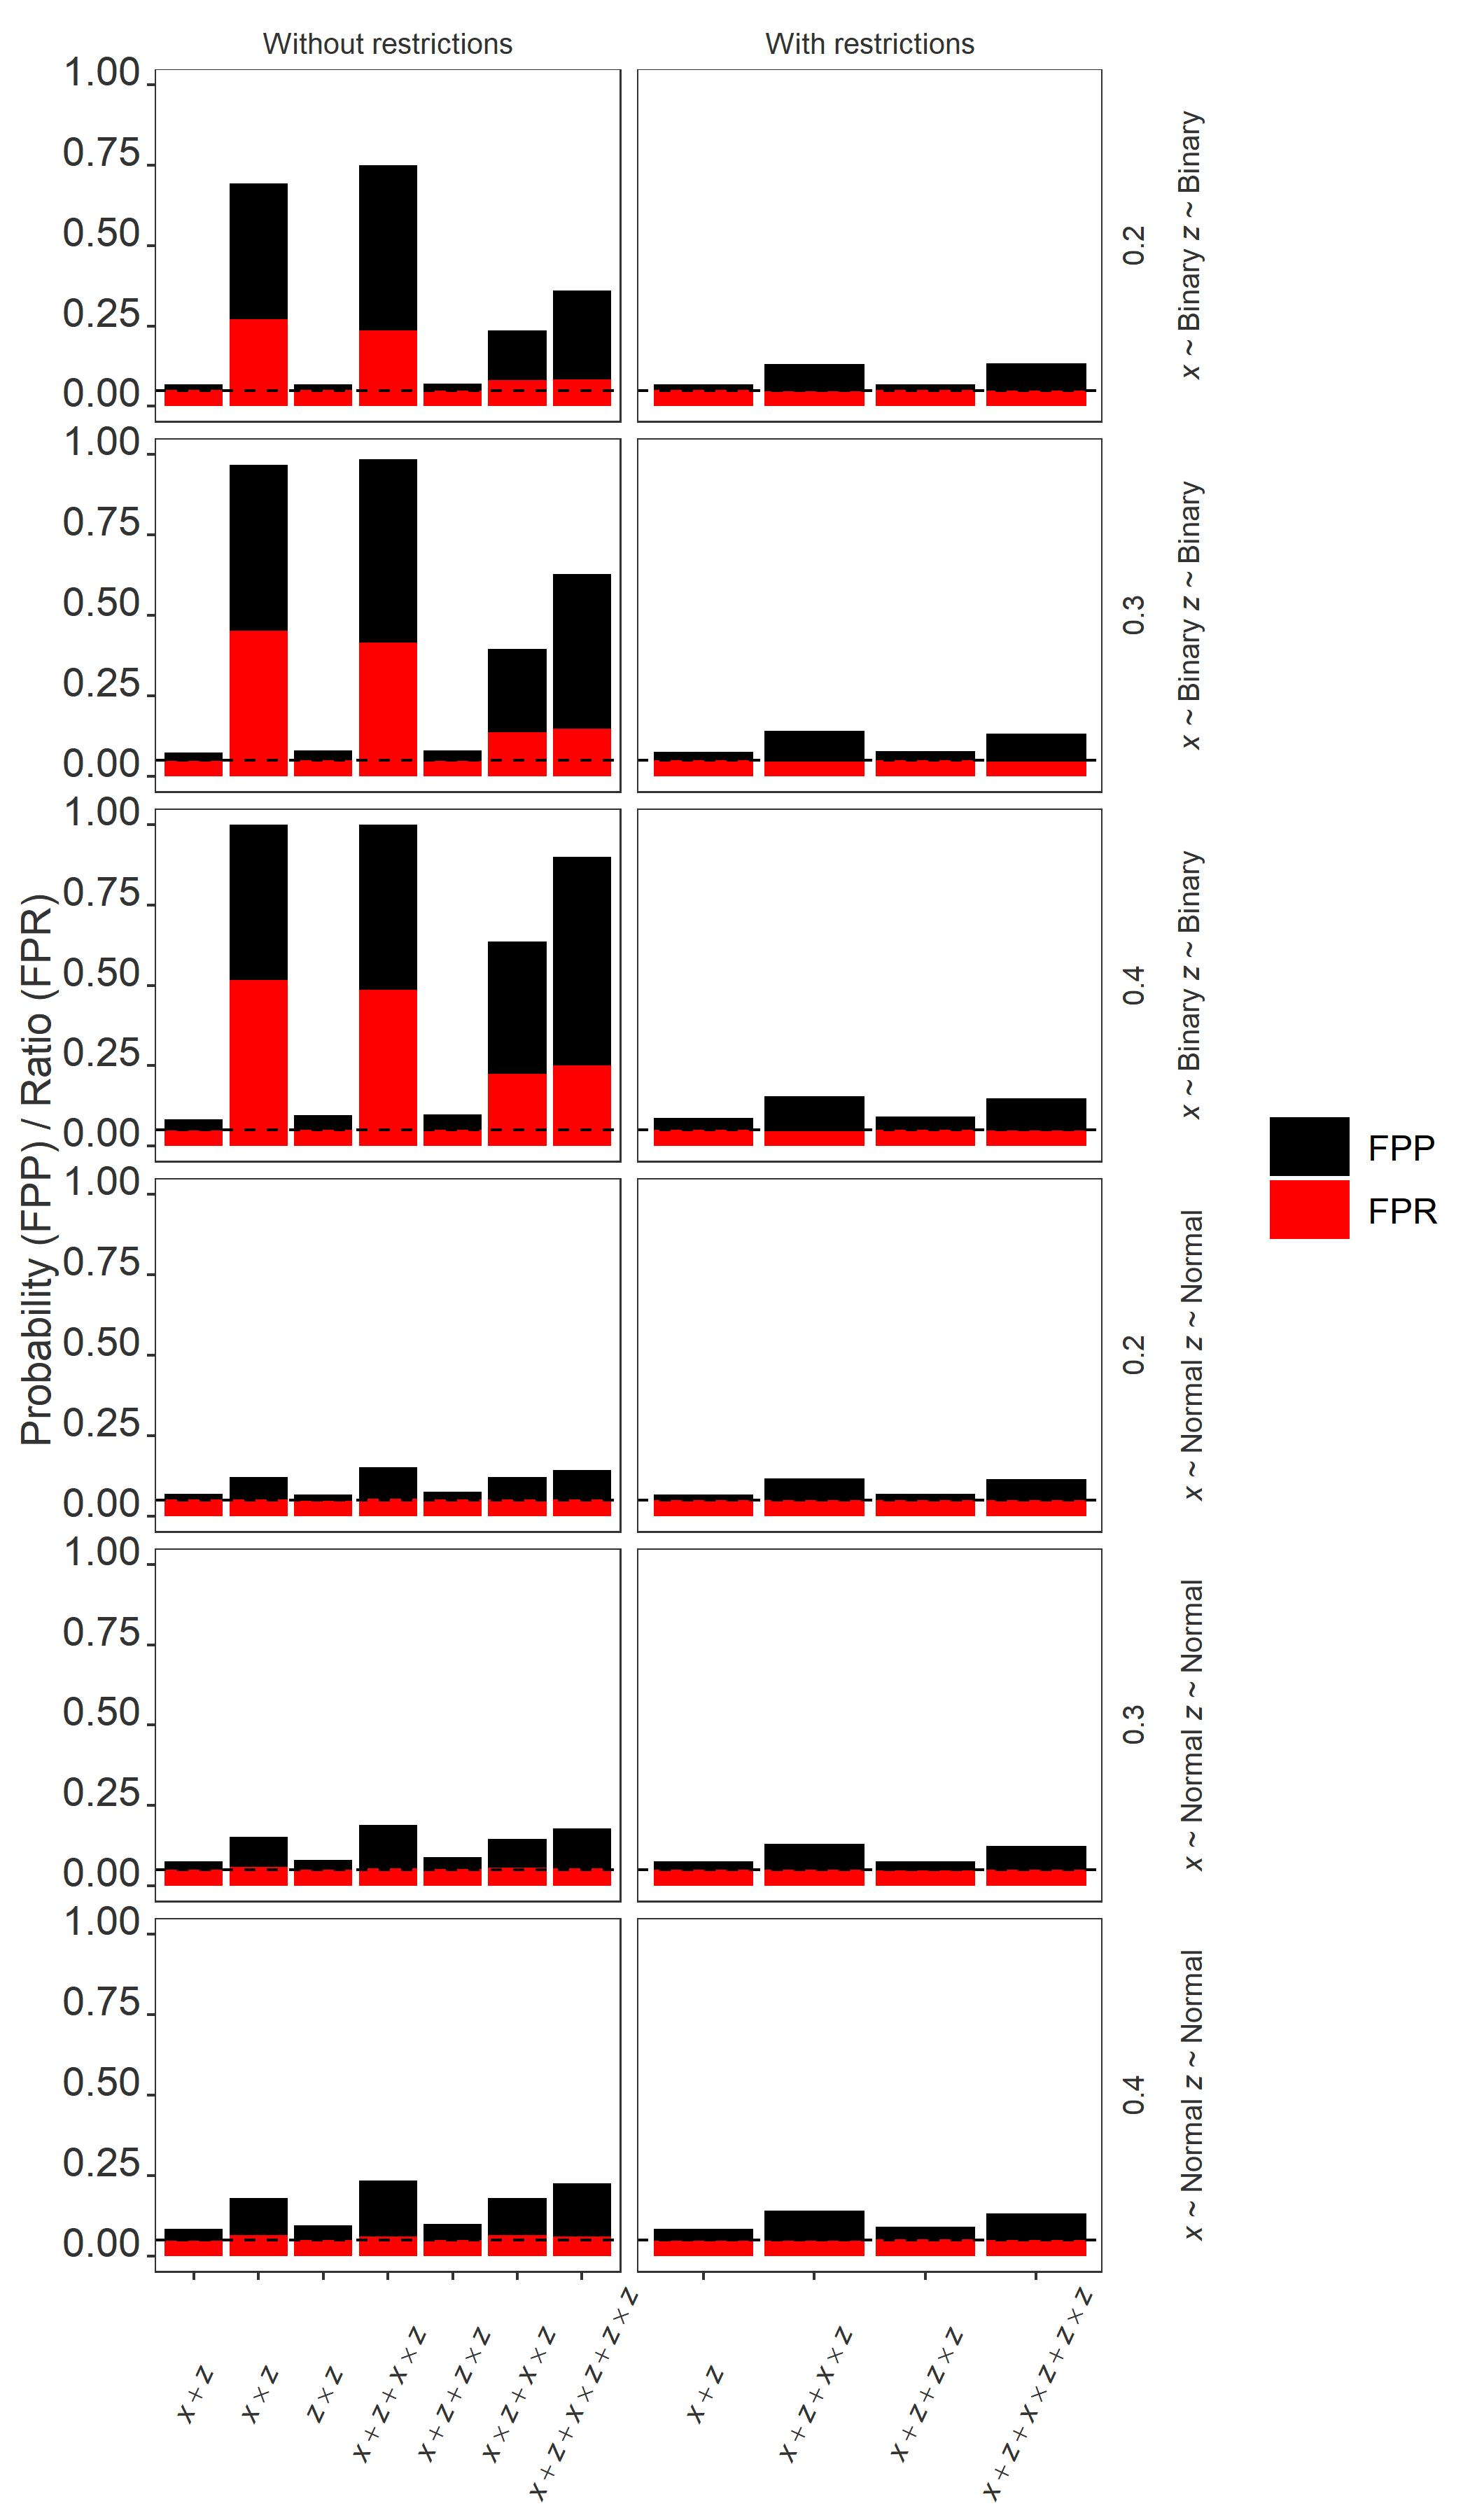
\includegraphics[scale=0.7]{R/Analysis/Result/Figures/Figure2SIBon.jpeg}
\centering
\caption{False positive probability and false positive for different levels of correlation between the dependent variable and the covariates ranging from  $\textit{r}=0.2$ to  $\textit{r}=0.4$ when using Bonferroni correction. Black denotes the false positive probability and red denotes the false positive ratio. Dashed blacked line indicates 0.05. The description of the figure is otherwise the same as for Figure \ref{fig:appfigure7}.}
\label{fig:appfigure8}
\end{figure}
\end{landscape}



\begin{figure}[hbt!]
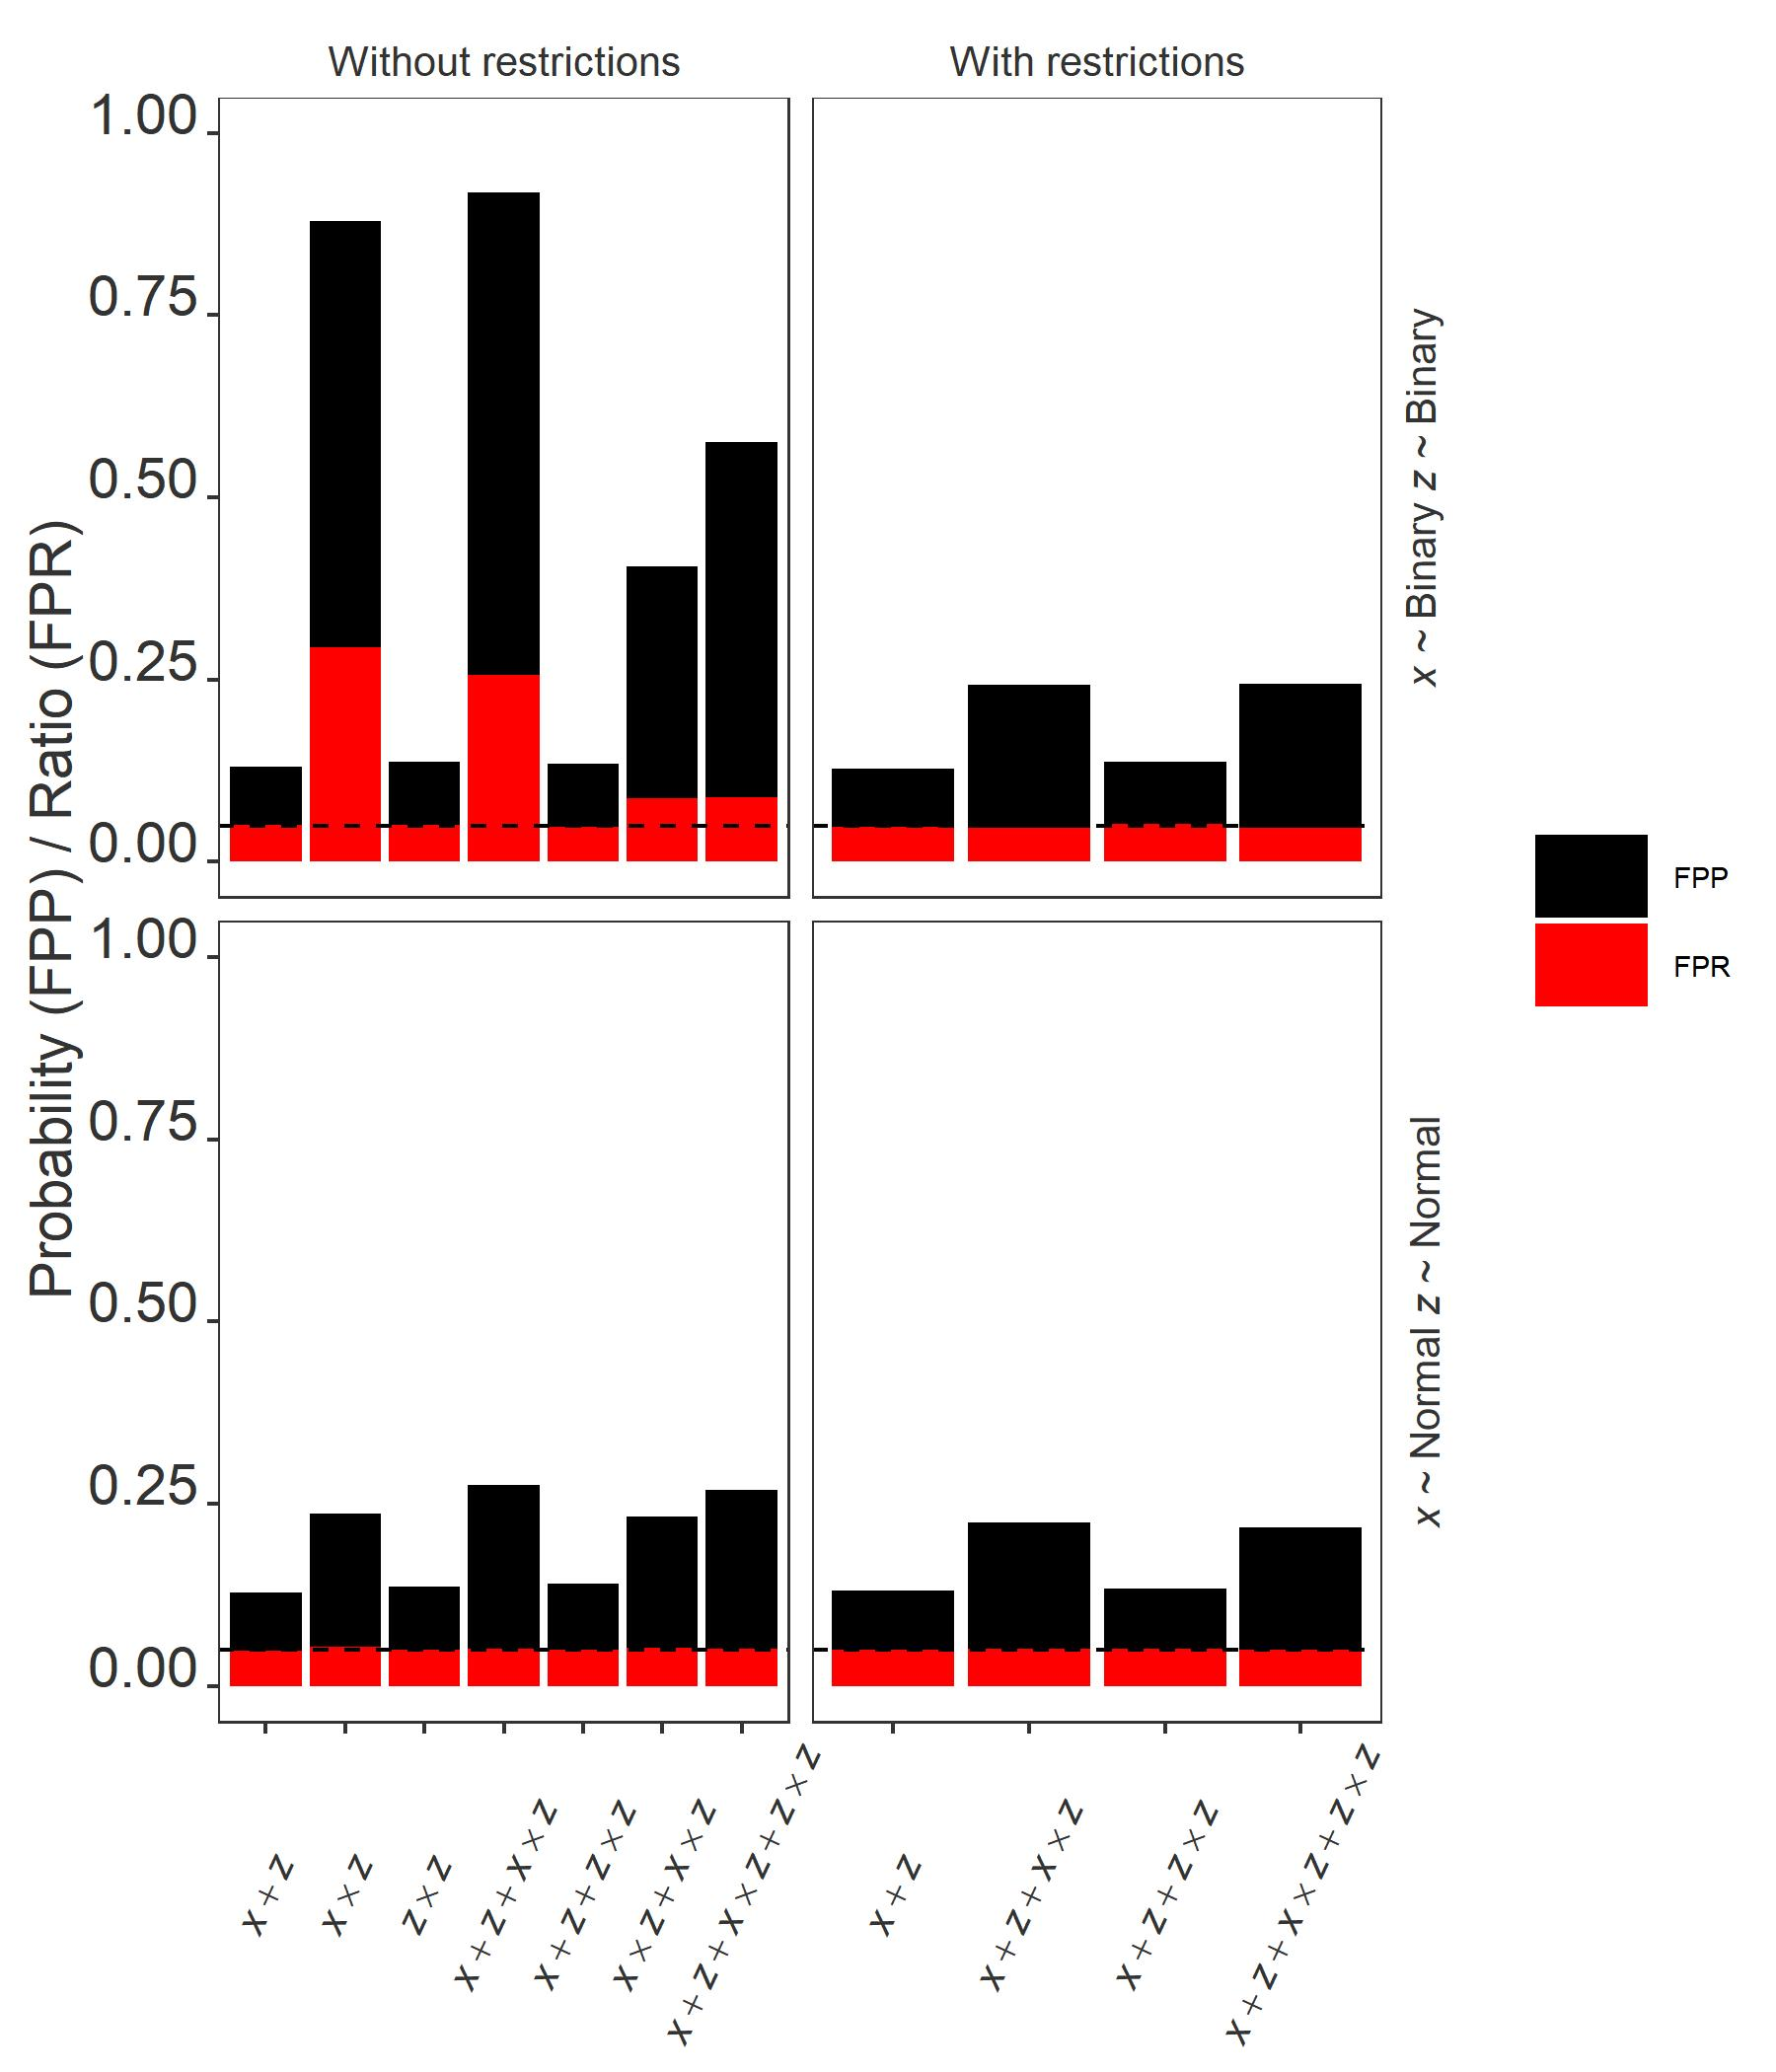
\includegraphics{R/Analysis/Result/Figures/Figure3SIBon.jpeg}
\centering
\caption{False positive probability and false positive ratio when using two dependent variables and the average of the two (meaning three dependent variables in total) when using Bonferroni correction. The correlation between the dependent variables is set to  $\textit{r}=0.5$ with the correlation between the dependent variables and covariates still at  $\textit{r}=0.2$. Black denotes the the false positive probability and red denotes the false positive ratio. Dashed blacked line indicates 0.05. The description of the figure is otherwise the same as for Figure \ref{fig:appfigure7}.}
\label{fig:appfigure9}
\end{figure}


\begin{figure}[hbt!]
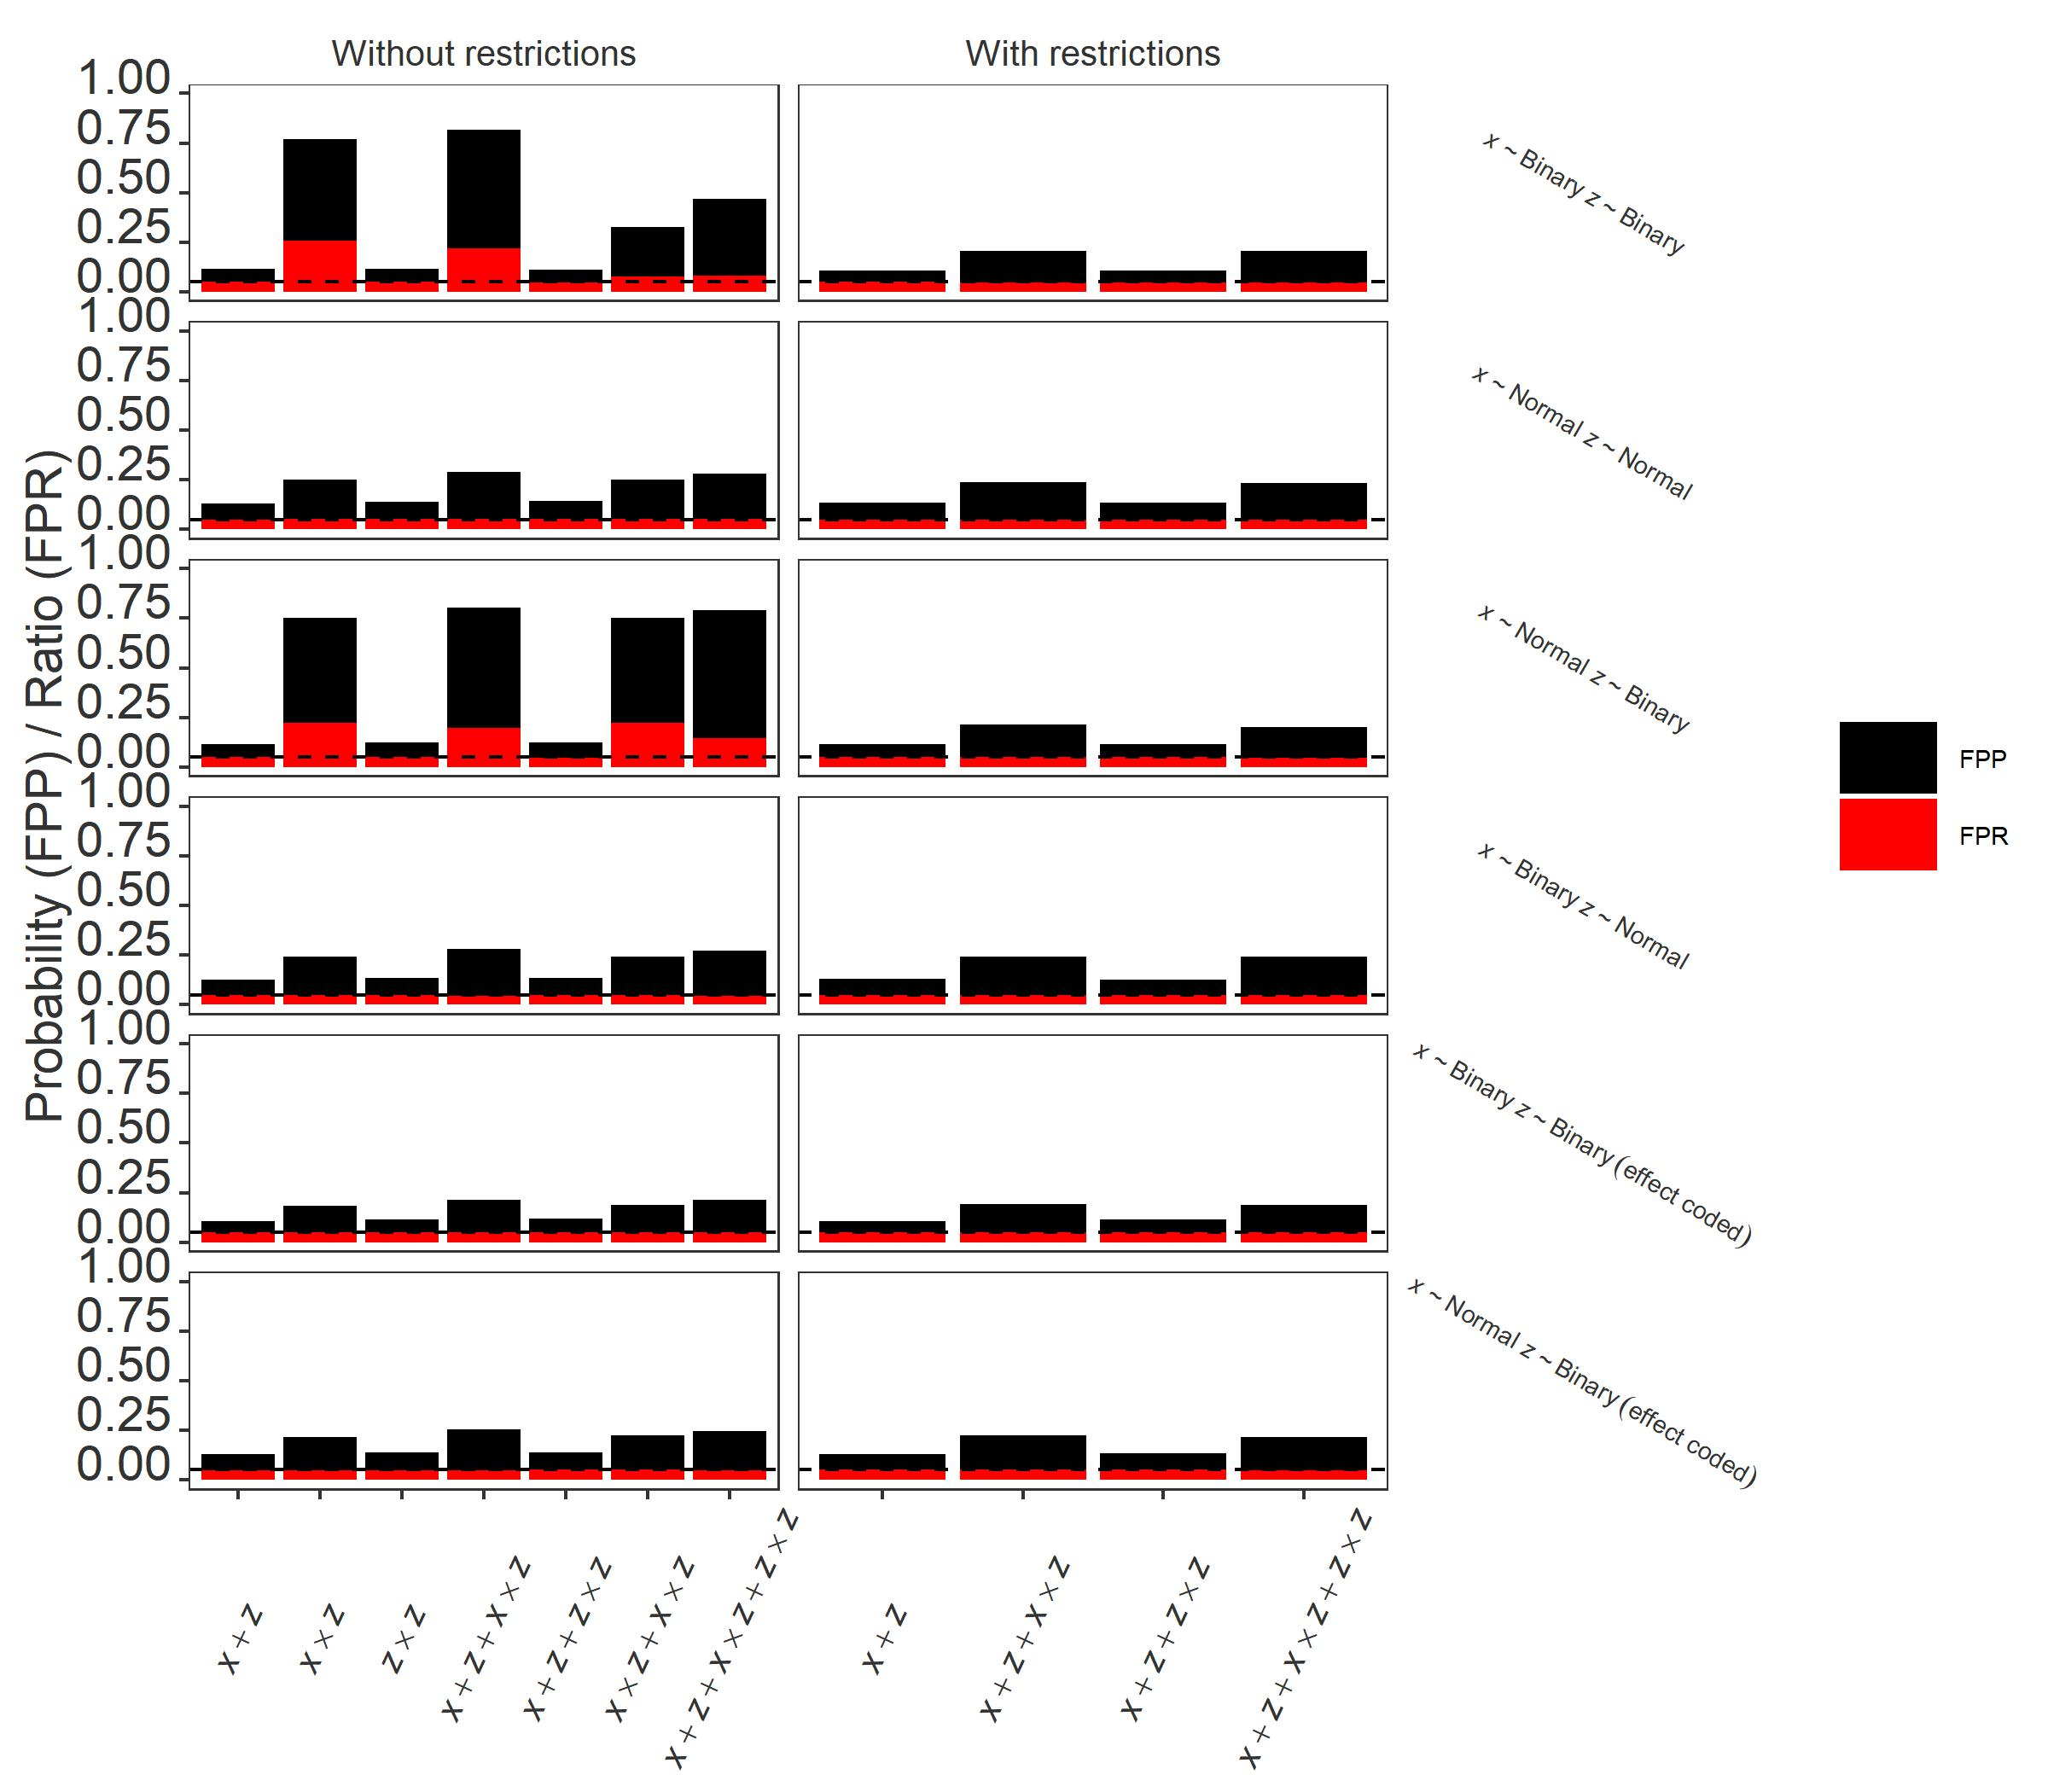
\includegraphics[scale=0.95]{R/Analysis/Result/Figures/Figure1BSIBon.jpeg}
\centering
\caption{False positive probability and false positive ratio when using multiple outlier criteria when using Bonferroni correction. Black denotes the the false positive probability and red denotes the false positive ratio. Dashed blacked line indicates 0.05. The description of the figure is otherwise the same as for Figure \ref{fig:appfigure7}.
}
\label{fig:appfigure10}
\end{figure}


\begin{figure}[hbt!]
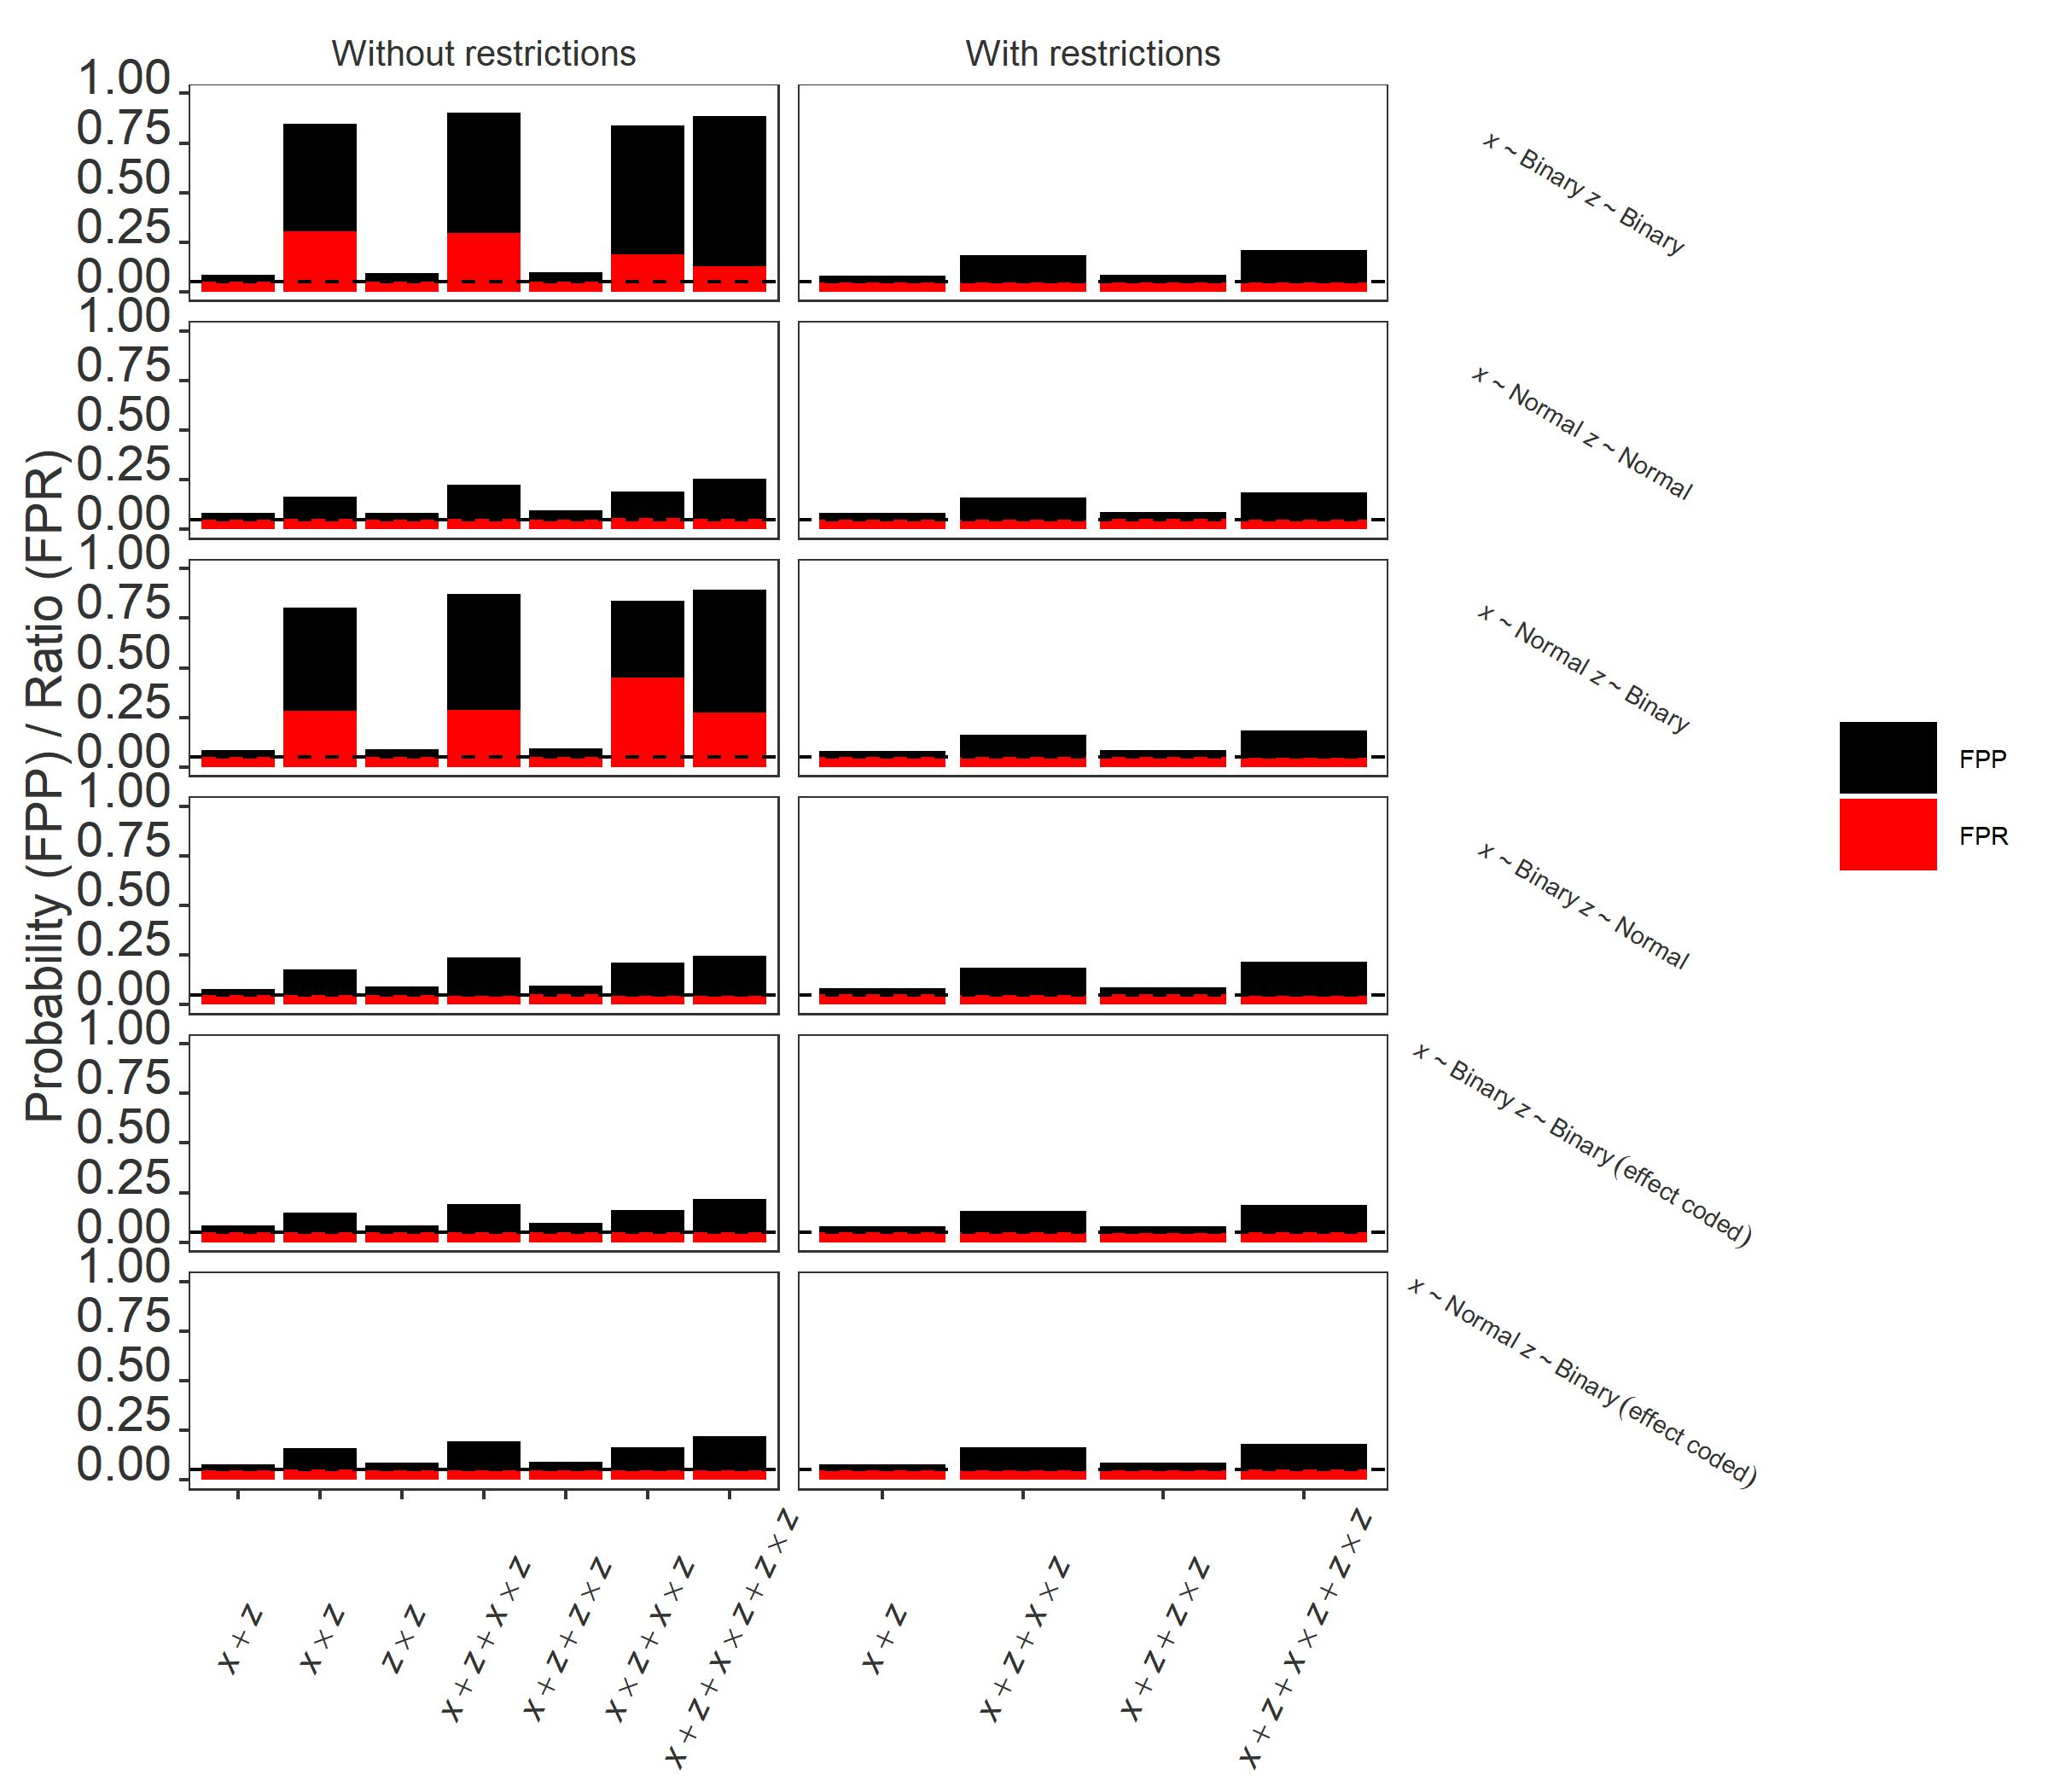
\includegraphics[scale=0.95]{R/Analysis/Result/Figures/Figure1CSIBon.jpeg}
\centering
\caption{False positive probability and false positive ratio when using three covariates instead of two as in the base line model and using Bonferroni correction. Black denotes the the false positive probability and red denotes the false positive ratio. Dashed blacked line indicates 0.05. The description of the figure is otherwise the same as for Figure \ref{fig:appfigure7}.
}
\label{fig:appfigure11}
\end{figure}


\begin{landscape}
\begin{figure}[hbt!]
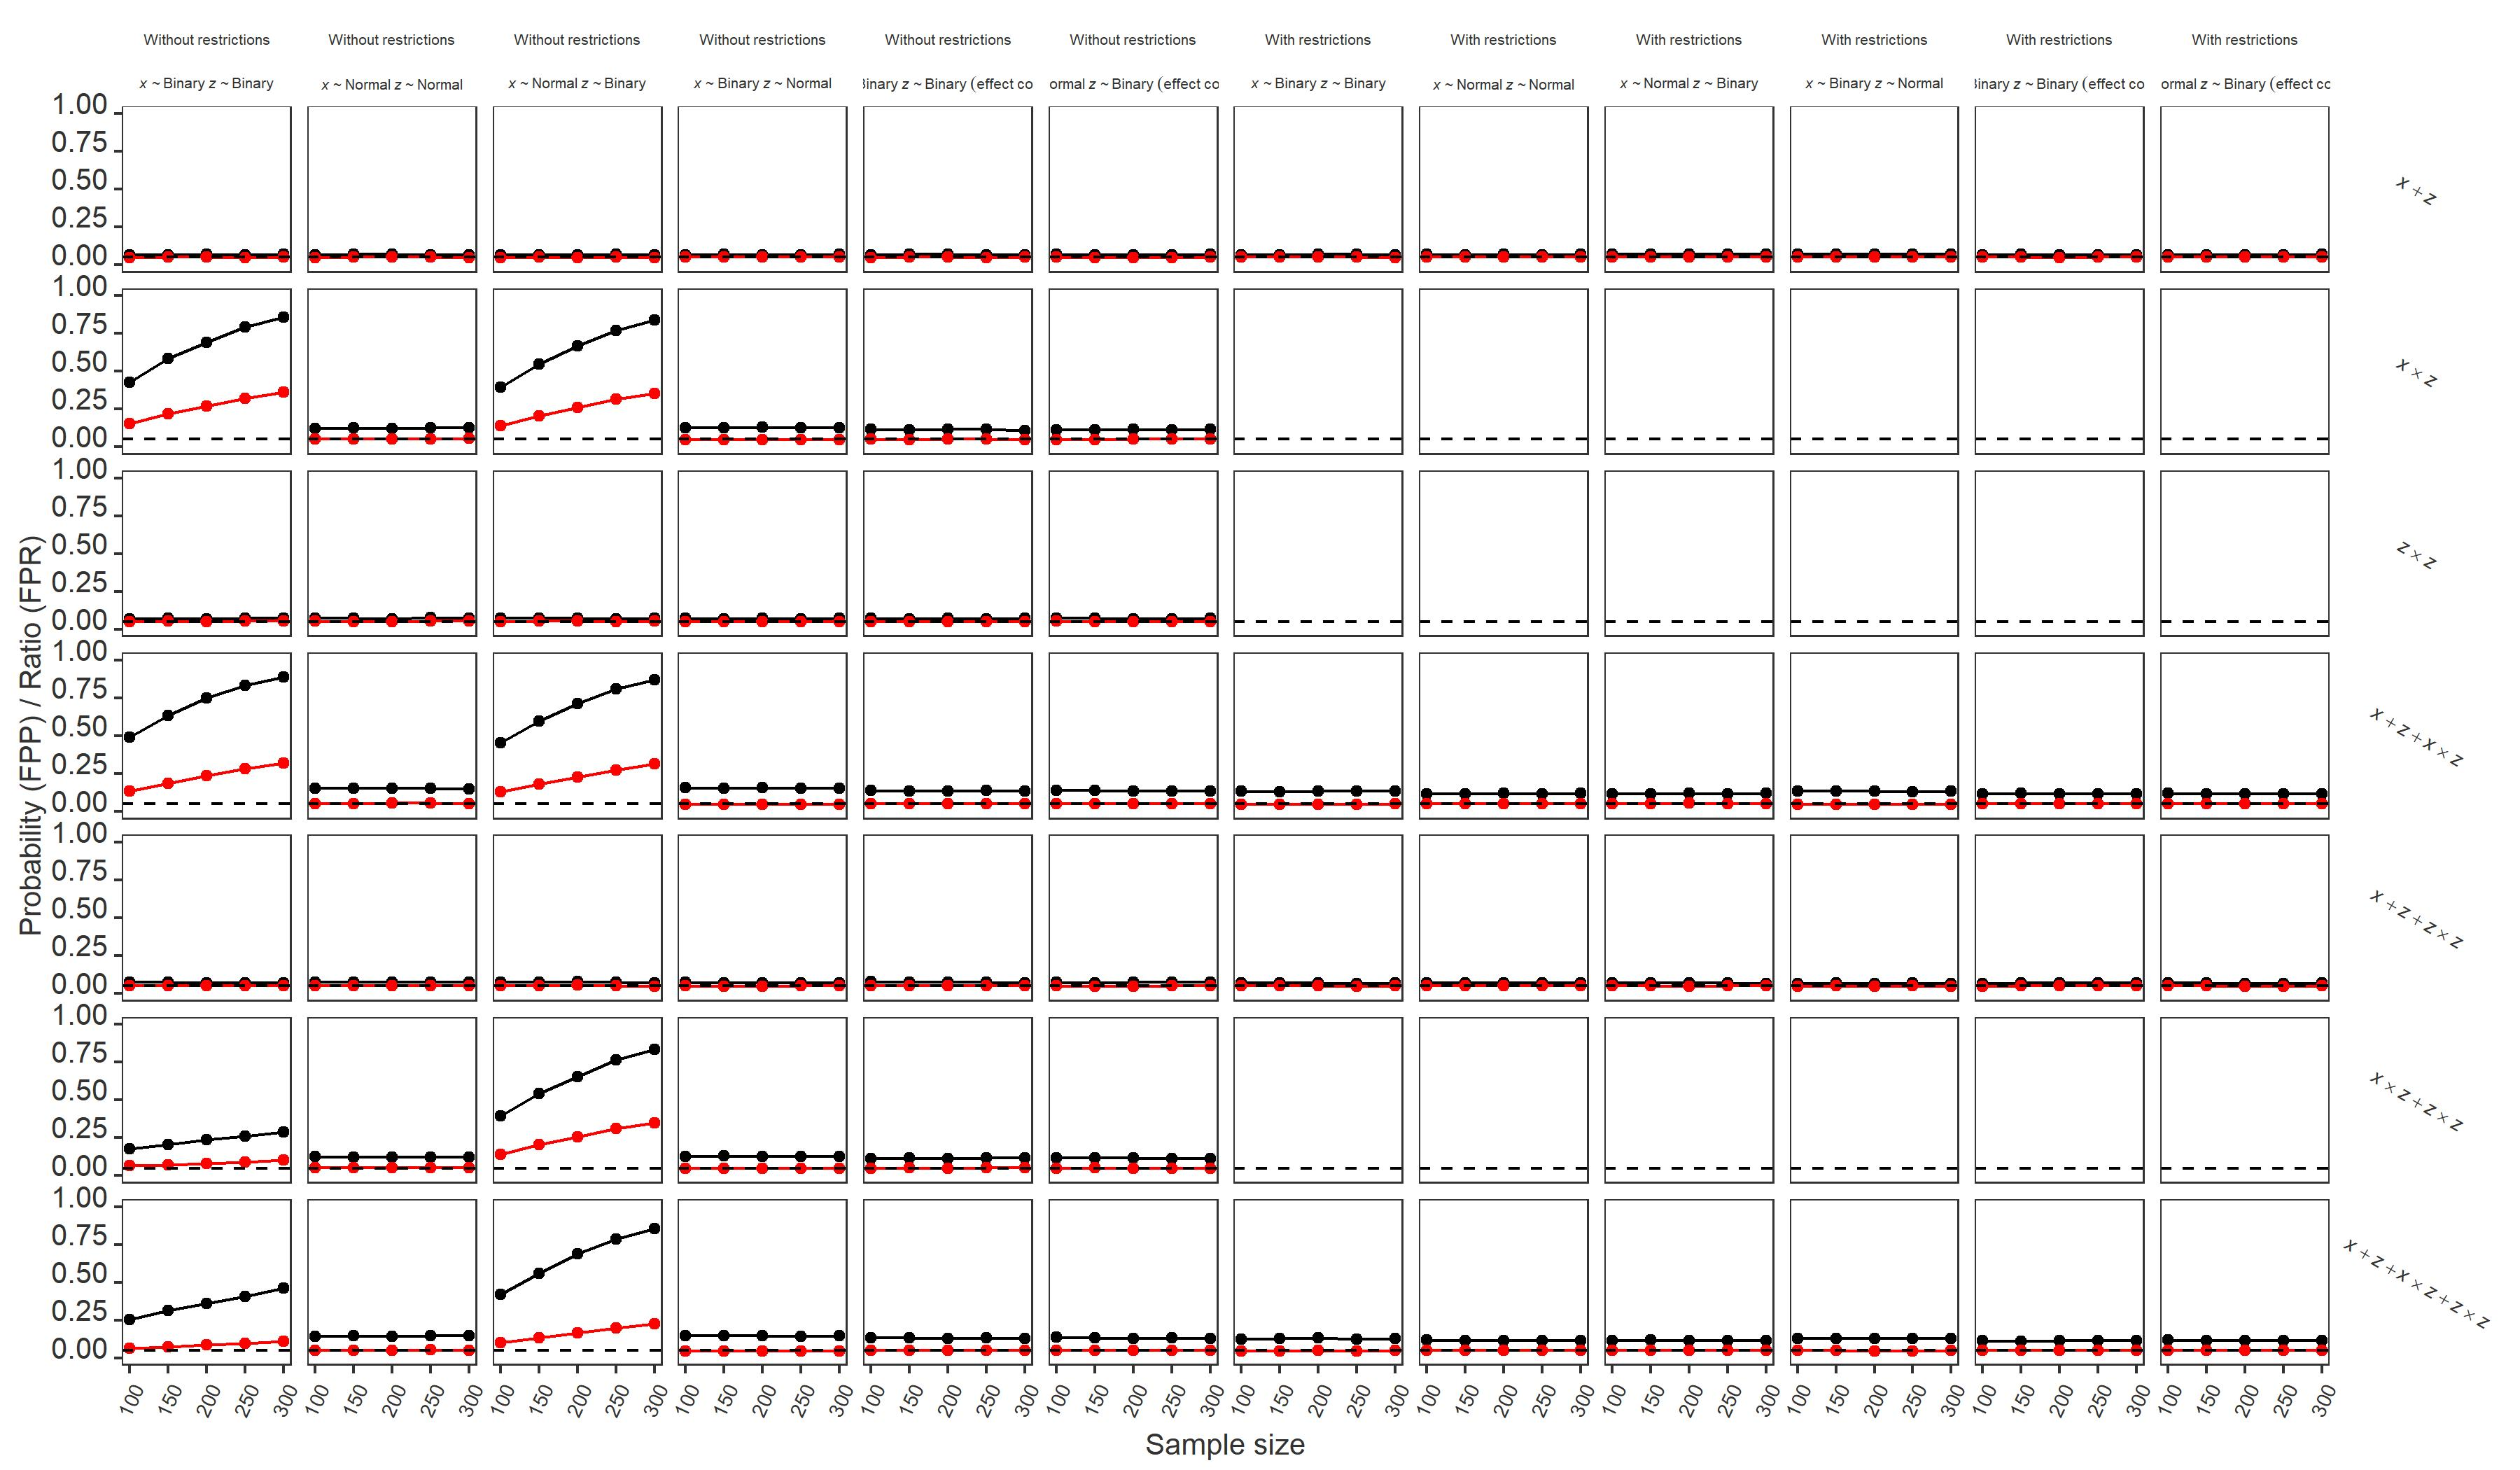
\includegraphics[scale=0.75]{R/Analysis/Result/Figures/Figure1DSIBon.jpeg}
\centering
\caption{Effect of increasing sample size for each model set and all combinations of data distributions (i.e., binary and normal) when using Bonferroni correction. Black denotes the false positive probability and red denotes the false positive ratio. Dashed blacked line indicates 0.05. The description of the figure is otherwise the same as for Figure \ref{fig:appfigure1}.}
\label{fig:appfigure12}
\end{figure}
\end{landscape}


\end{document}